\documentclass[14pt, t]{beamer}
\usepackage[T1]{fontenc}
\usepackage{graphicx}
\usepackage{multimedia}
\usepackage{amsmath, amssymb, mathtools}
\usepackage{bm, physics, siunitx}

\sisetup{separate-uncertainty=true, exponent-product=\cdot}
\graphicspath{{../media}}

% BEGIN BIBLIOGRAPHY CONFIGURATION
% --------------------------------------------- %
\usepackage[maxcitenames = 2, backend=biber]{biblatex}
\usepackage{../bib/atlasbiblatex}
\addbibresource{../bib/sources.bib}
\renewcommand{\bibfont}{\footnotesize}
\setbeamertemplate{bibliography item}{\insertbiblabel}  % to print reference numbers and not icons
% --------------------------------------------- %
% END BIBLIOGRAPHY CONFIGURATION


% BEGIN BEAMER CONFIGURATION
% -------------------------------------- %
\setbeamertemplate{navigation symbols}{}
\usefonttheme{serif}
% \setbeamertemplate{footline}[frame number]
\setbeamertemplate{footline}{\raisebox{5.5pt}{\makebox[\paperwidth]{\hfill \makebox[20pt]{\scriptsize \insertframenumber}}}}
% -------------------------------------- %
% END BEAMER CONFIGURATION


% BEGIN CUSTOM MACROS
% --------------------------------------------- %
\definecolor{myMaroon}{RGB}{96,0,6}
\newcommand{\myhref}[2]{\hyperref[#1]{\textcolor{blue}{\underline{#2}}}}
\newcommand{\myurl}[1]{\textcolor{blue}{\texttt{\url{#1}}}}
\newcommand{\chem}[1]{\ensuremath{\mathrm{#1}}}

\newcommand{\diff}{\mathop{}\!\mathrm{d}}
\renewcommand{\vec}[1]{\bm{#1}}
\newcommand{\mat}[1]{\mathbf{#1}}
\newcommand{\tensor}[1]{\mathsf{#1}}
\newcommand{\uvec}[1]{\hat{\vec{#1}}}
\renewcommand{\grad}{\nabla}

\newcommand{\X}{\mat{X}}
\newcommand{\W}{\mat{W}}
\newcommand{\x}{\vec{x}}
\newcommand{\y}{\vec{y}}
\newcommand{\w}{\vec{w}}
\renewcommand{\b}{\vec{b}}
\newcommand{\z}{\vec{z}}
\renewcommand{\a}{\vec{a}}

\newcommand{\subgrad}[1]{\grad_{\mspace{-4mu}#1}\mspace{1mu}} % gradient with a subscript
\newcommand{\supgrad}[2]{\grad_{\mspace{-4mu}#1}\mspace{1mu}^{\mspace{-4mu}#2}} % gradient with a subscript and superscript
% --------------------------------------------- %
% END CUSTOM MACROS


\begin{document}

\begin{frame}[plain]
    \begin{center}

    \definecolor{ul-red}{RGB}{220,29,39}
    \small{\textsc{University of Ljubljana}}\\
    \small{\textsc{Faculty of {\color{ul-red} Mathematics and Physics}}}\\[1mm]
    \footnotesize{\textsc{Department of Physics}}\\
    \vspace{2mm}
    \large{Seminar}\\
    \vspace{-2mm}
    \rule{\textwidth}{0.2pt}\\[3mm]

    {\Large \textbf{End-to-End Classification}} \\[-1mm]
    {\small \textbf{for Discovery of New Processes}}\\[-2mm]
    {\small \textbf{in High-Energy Physics}}

    \vspace{-1mm}
    \rule{\textwidth}{0.2pt}\\[3mm]

    \vspace{5mm}

    \scriptsize{\textsc{Author:} Elijan Mastnak}\\
    \scriptsize{\textsc{Adviser:} prof. dr. Borut Paul Ker\v{s}evan}\\

    \end{center}
    
\end{frame}

% \begin{frame}
% \frametitle{Contents}
% \tableofcontents
% \end{frame}

\section{What is End-to-End Classification?}

\begin{frame}
    \frametitle{What is Particle Classification?}

    \begin{block}{Classification}
        Two high-energy particles collide. Which particles were produced as a result of the collision?
    \end{block}

    \pause
    \vspace{2mm}
    We will consider \textit{binary} Higgs boson classification: \\
    \begin{itemize}
    
        \item Higgs boson (\textit{signal})

        \item anything else (\textit{background})
    
    \end{itemize}
    \vspace{-5mm}
    \begin{figure}
        \centering
        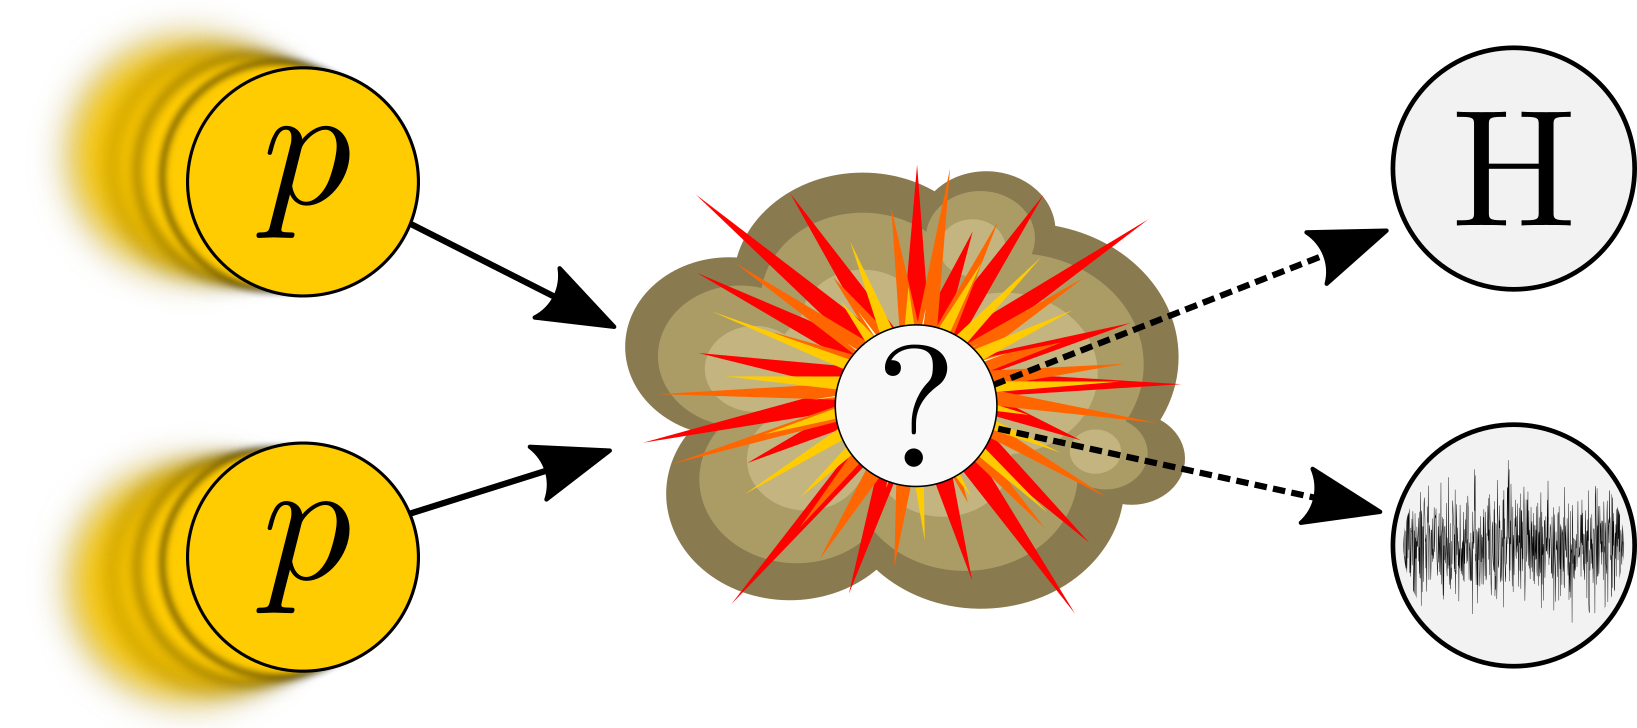
\includegraphics[width=0.65\linewidth]{vector/figures-presentation/classification.png}
    \end{figure}
    % explosion source: https://2dgameartguru.com/back-with-a-bang-creating-explosions/
\end{frame}

\begin{frame}
\frametitle{End-to-End Classification}

    \begin{itemize}
    
        \item<1-> Directly uses raw detector data

        \item<2-> Eliminates complicated intermediate steps

    \end{itemize}

    \only<1>{
    \begin{figure}
        \centering
        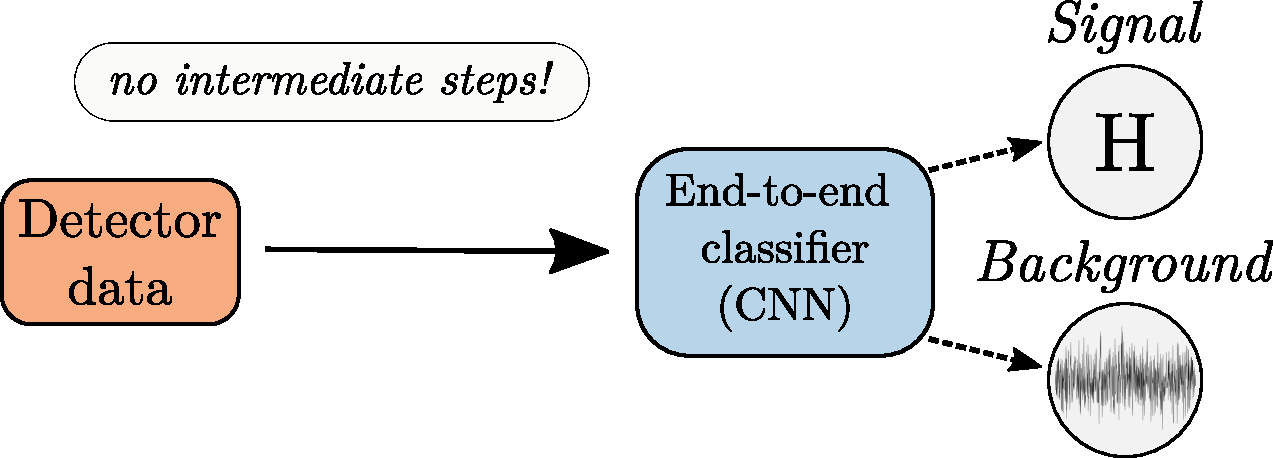
\includegraphics[width=\linewidth]{vector/figures-presentation/workflow-end-end.pdf}
    \end{figure}}
    
    \only<2>{
    \begin{figure}
        \centering
        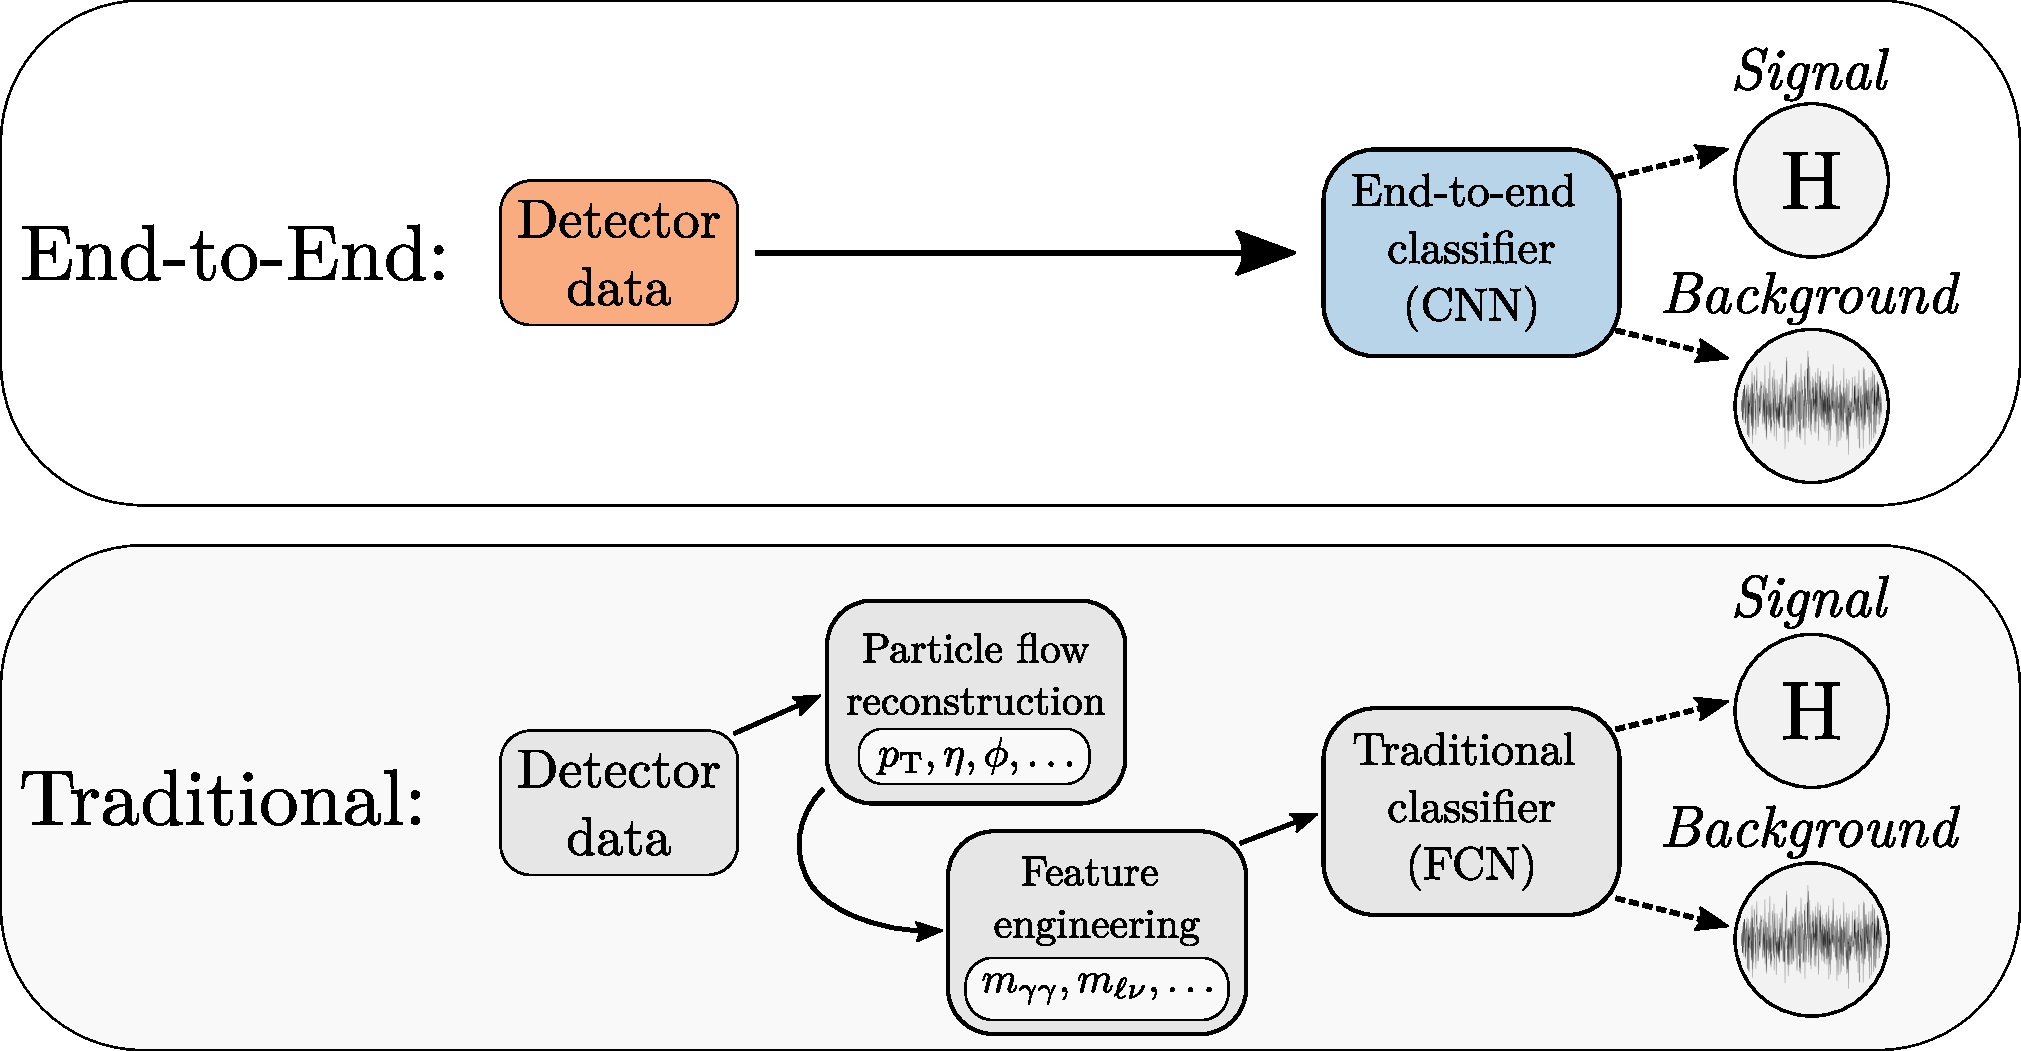
\includegraphics[width=\linewidth]{vector/figures-presentation/workflow-both.pdf}
    \end{figure}}

\end{frame}



\section{Producing and Measuring Collision Data}
\begin{frame}
\frametitle{What is the Detector Data?}

The set of measured physical quantities describing the products of a particle collision

\vspace{2mm}
\begin{itemize}

    % \item Quantitative description of particle collisions

    \item Produced by: Large Hadron Collider (LHC)

    \item Measured by: Compact Muon Solenoid (CMS)

\end{itemize}
\vspace{4mm}
We will explain:
\begin{enumerate}

    \item proton acceleration and collision at the LHC

    \item physical principles of CMS subdetectors

    \item how to interpret CMS detector data

\end{enumerate}
    
\end{frame}

\begin{frame}
    \frametitle{Proton Acceleration at the LHC}
    \begin{columns}
        \column{0.4\textwidth}
        Sequence:
        \begin{enumerate}
        
            \item hydrogen ions

            \item boosting stages

            \item LHC

            \item nominal collisions points

            \item detectors
        
        \end{enumerate}

        \column{0.6\textwidth}
        \begin{figure}[t!]
            \centering
            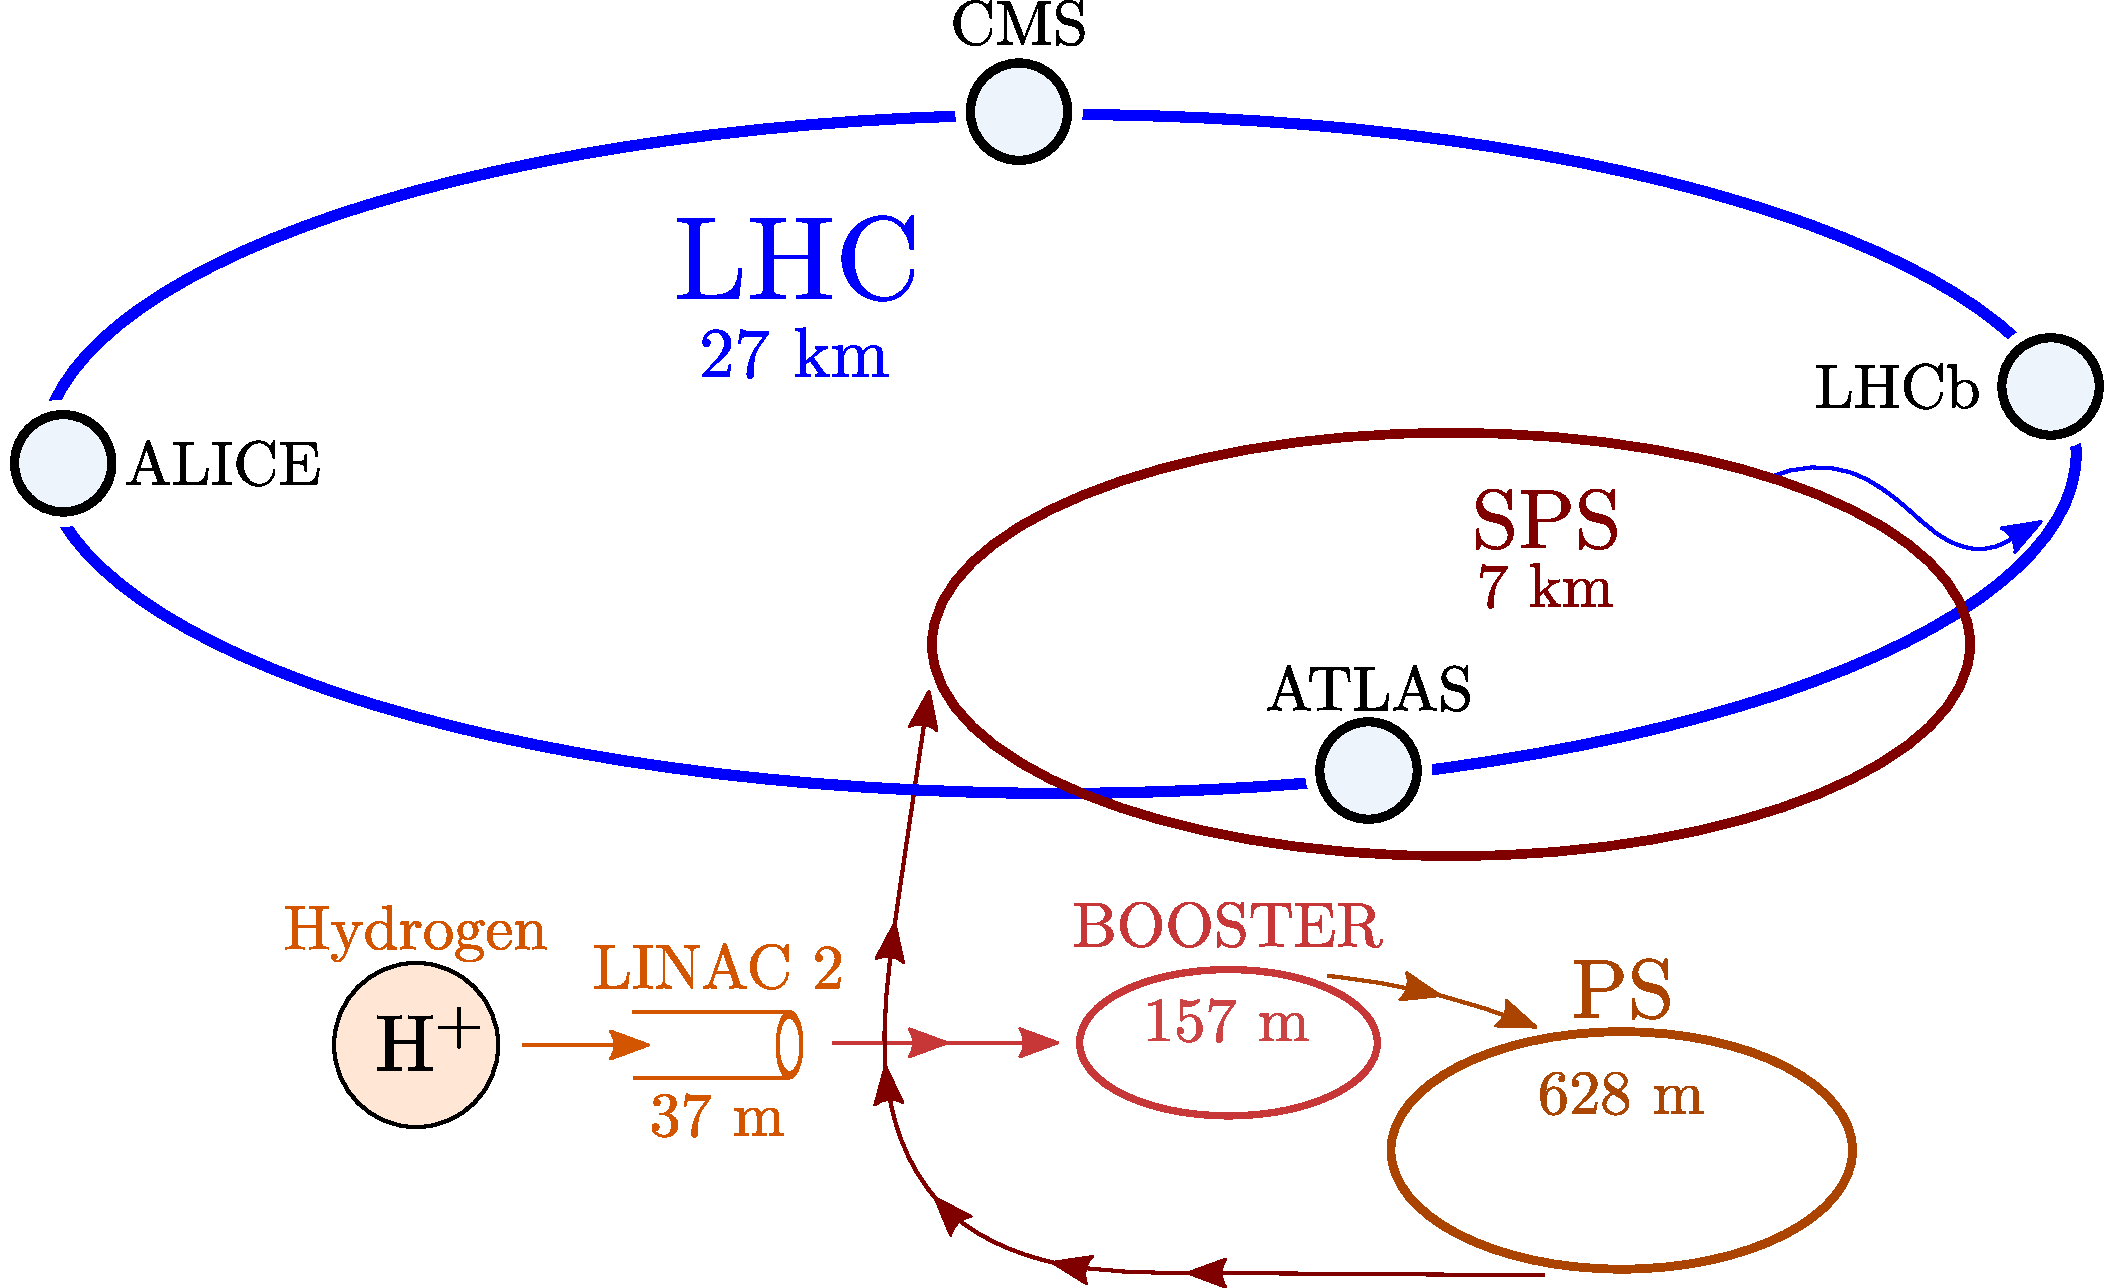
\includegraphics[width=\columnwidth]{vector/cern-complex.pdf}
        \end{figure}
        \vspace{-3mm}
        \hfill
        \tiny{Adapted from \cite{image-cern-complex}}
        
    \end{columns}

    \vspace{3mm}
    $ \sim \SI{7}{\tera \electronvolt} $ proton energy\\
    $ \sim 10^{11} $ particles per bunch\\
    $ \sim \SI{25}{\nano \second} $ between collisions
    
\end{frame}

\begin{frame}
% some facts and figures:
% https://www.lhc-closer.es/taking_a_closer_look_at_lhc/0.lhc_p_collisions
% nice cern brochure in everyday language
% https://cds.cern.ch/record/2255762/files/CERN-Brochure-2017-002-Eng.pdf
\frametitle{Collision}
    \begin{itemize}
    
        \item Two protons (rarely!) collide head-on

        \item Chain of secondary interactions

        \item Resulting particles are the \textit{decay signature}
    
    \end{itemize}

    \begin{figure}
        \centering
        \includegraphics[width=\linewidth]{vector/figures-presentation/collision.png}
    \end{figure}
\end{frame}

\begin{frame}[plain]

    \vspace{2mm}
    \begin{center}
    \makebox[\textwidth][c]{\movie{\includegraphics[width=\paperwidth]{../media/animations/collision.png}}{../media/animations/collision.ogv}}

     % https://video.online-convert.com/convert-to-ogv 
        % \makebox[\textwidth][c]{\movie{\includegraphics[width=\paperwidth]{\mediadirectory/animations/test.png}}{\mediadirectory/animations/test.ogv}}

        {\small Video: proton-proton collision at the ATLAS detector \cite{anim-atlas}}
    \end{center}

\end{frame}

\begin{frame}

    \frametitle{An Important Limitation}

    \begin{itemize}
    
        \item Interesting particles decay \textit{rapidly} \hfill ($ \tau_{H} \sim \SI{e-22}{\second} $)

        \item \textit{We cannot detect a Higgs directly}

        \item \textit{All we see is the decay signature}
    
    \end{itemize}

    \begin{figure}
        \centering
        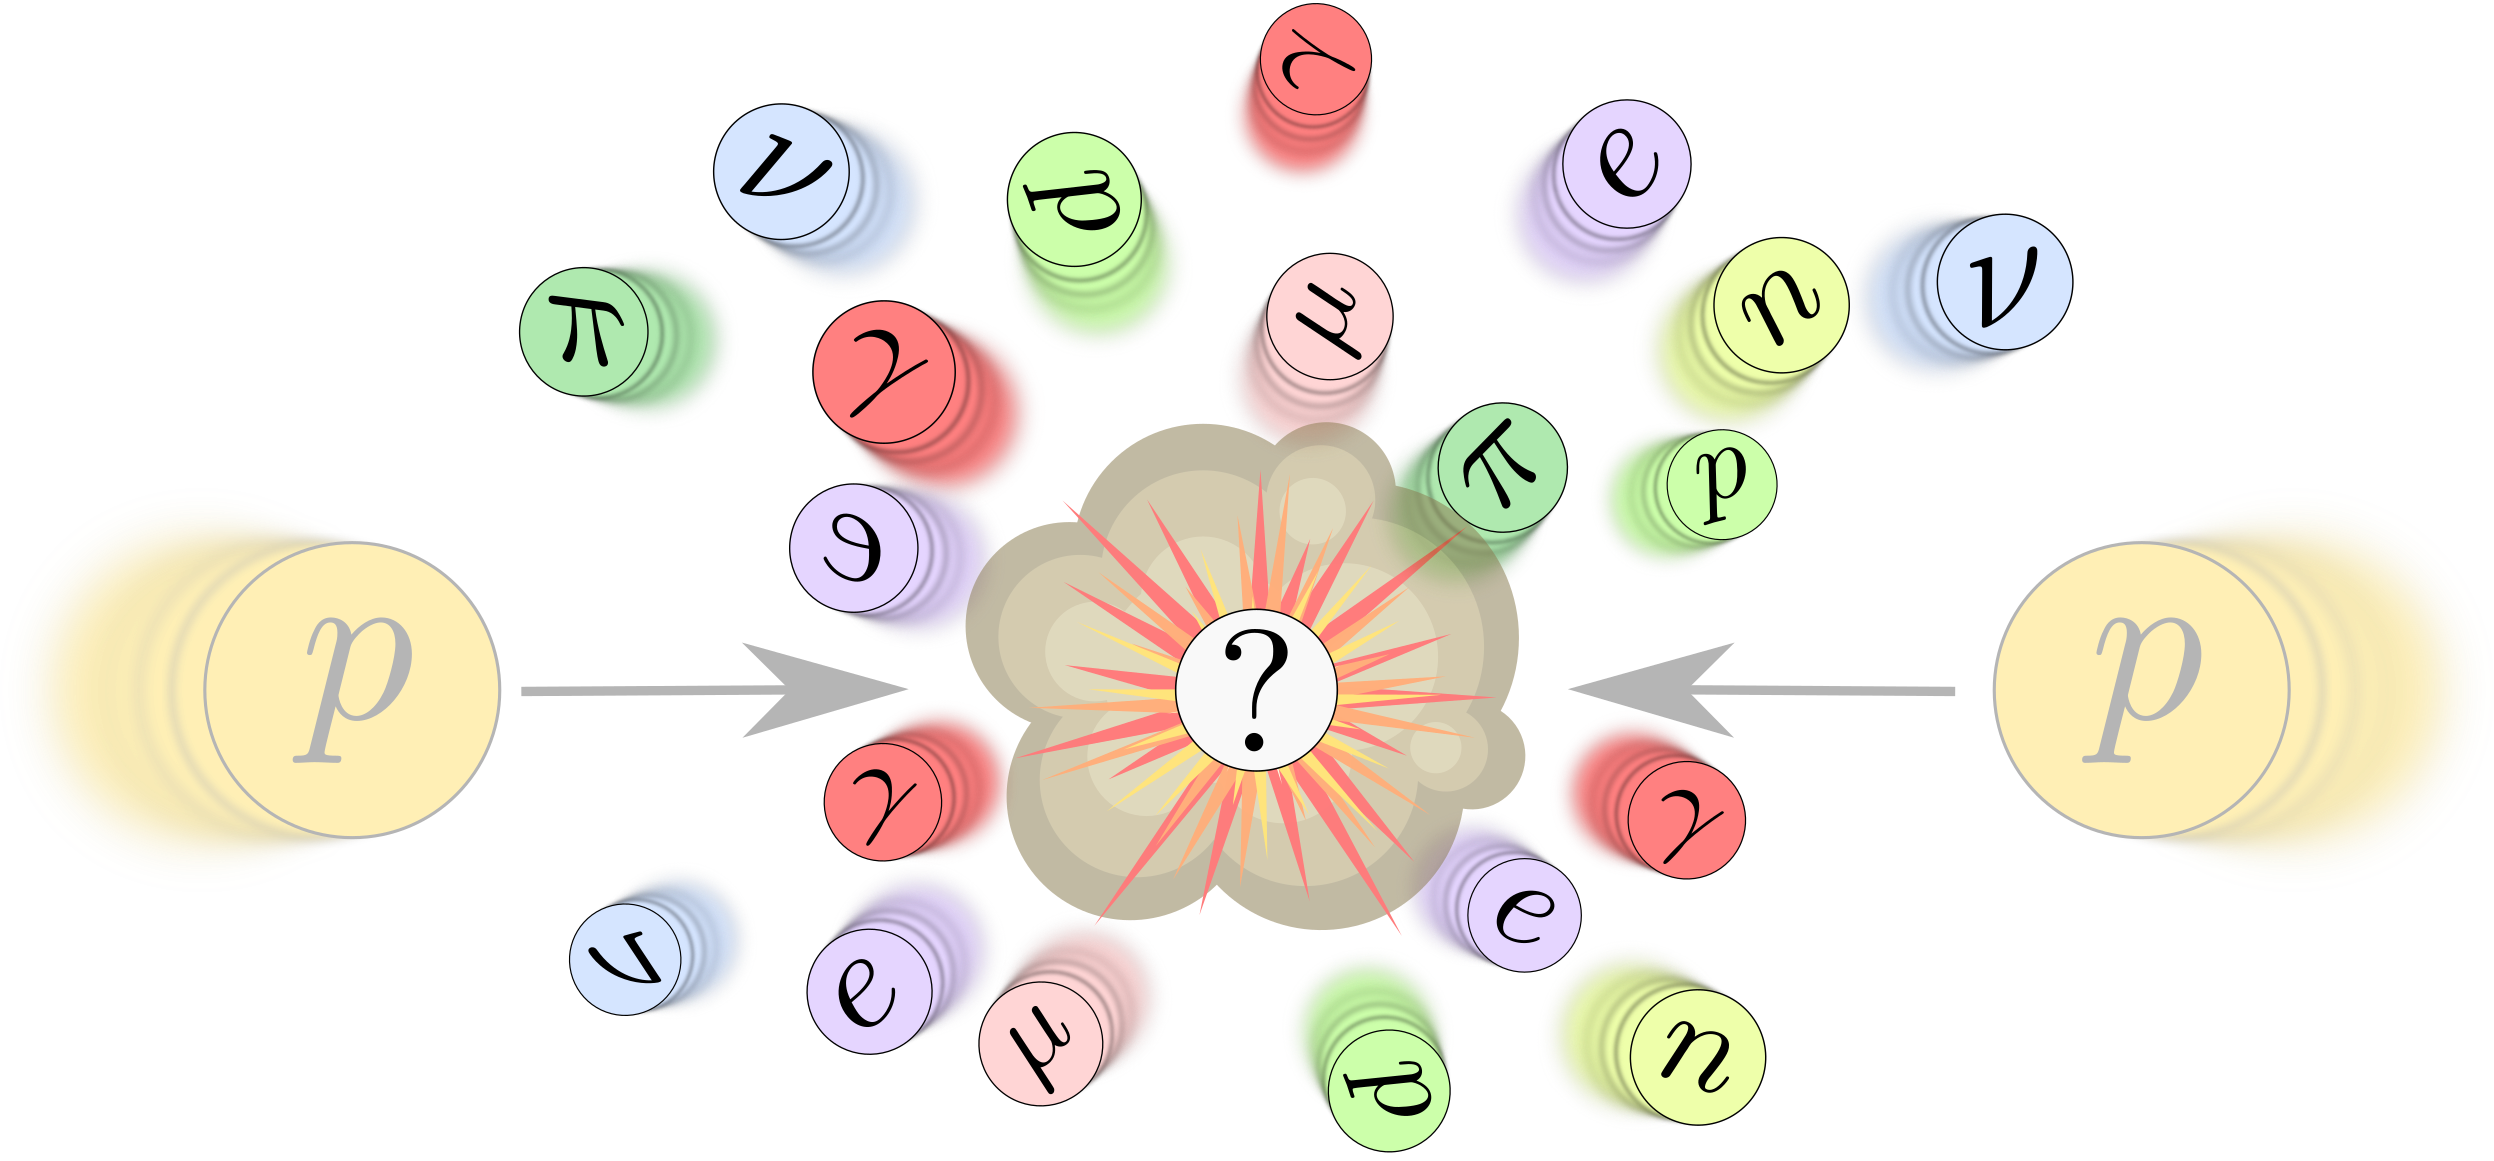
\includegraphics[width=\linewidth]{vector/figures-presentation/collision-question.png}
    \end{figure}

\end{frame}

\begin{frame}
    \frametitle{Quantifying a Decay Signature}
    A particle detector measures:
    \begin{itemize}
    
        \item particle trajectory (using \textit{trackers})

        \item particle energy (using \textit{calorimeters})
    
    \end{itemize}
    \vspace{5mm}
    With detector data, we can reconstruct:
    \begin{itemize}
    
        \item particle identity

        \item particle momentum

        \item production and decay vertices...
    
    \end{itemize}

\end{frame}

\begin{frame}
    \frametitle{The Compact Muon Solenoid}
    \begin{figure}[htb!]
        \centering
        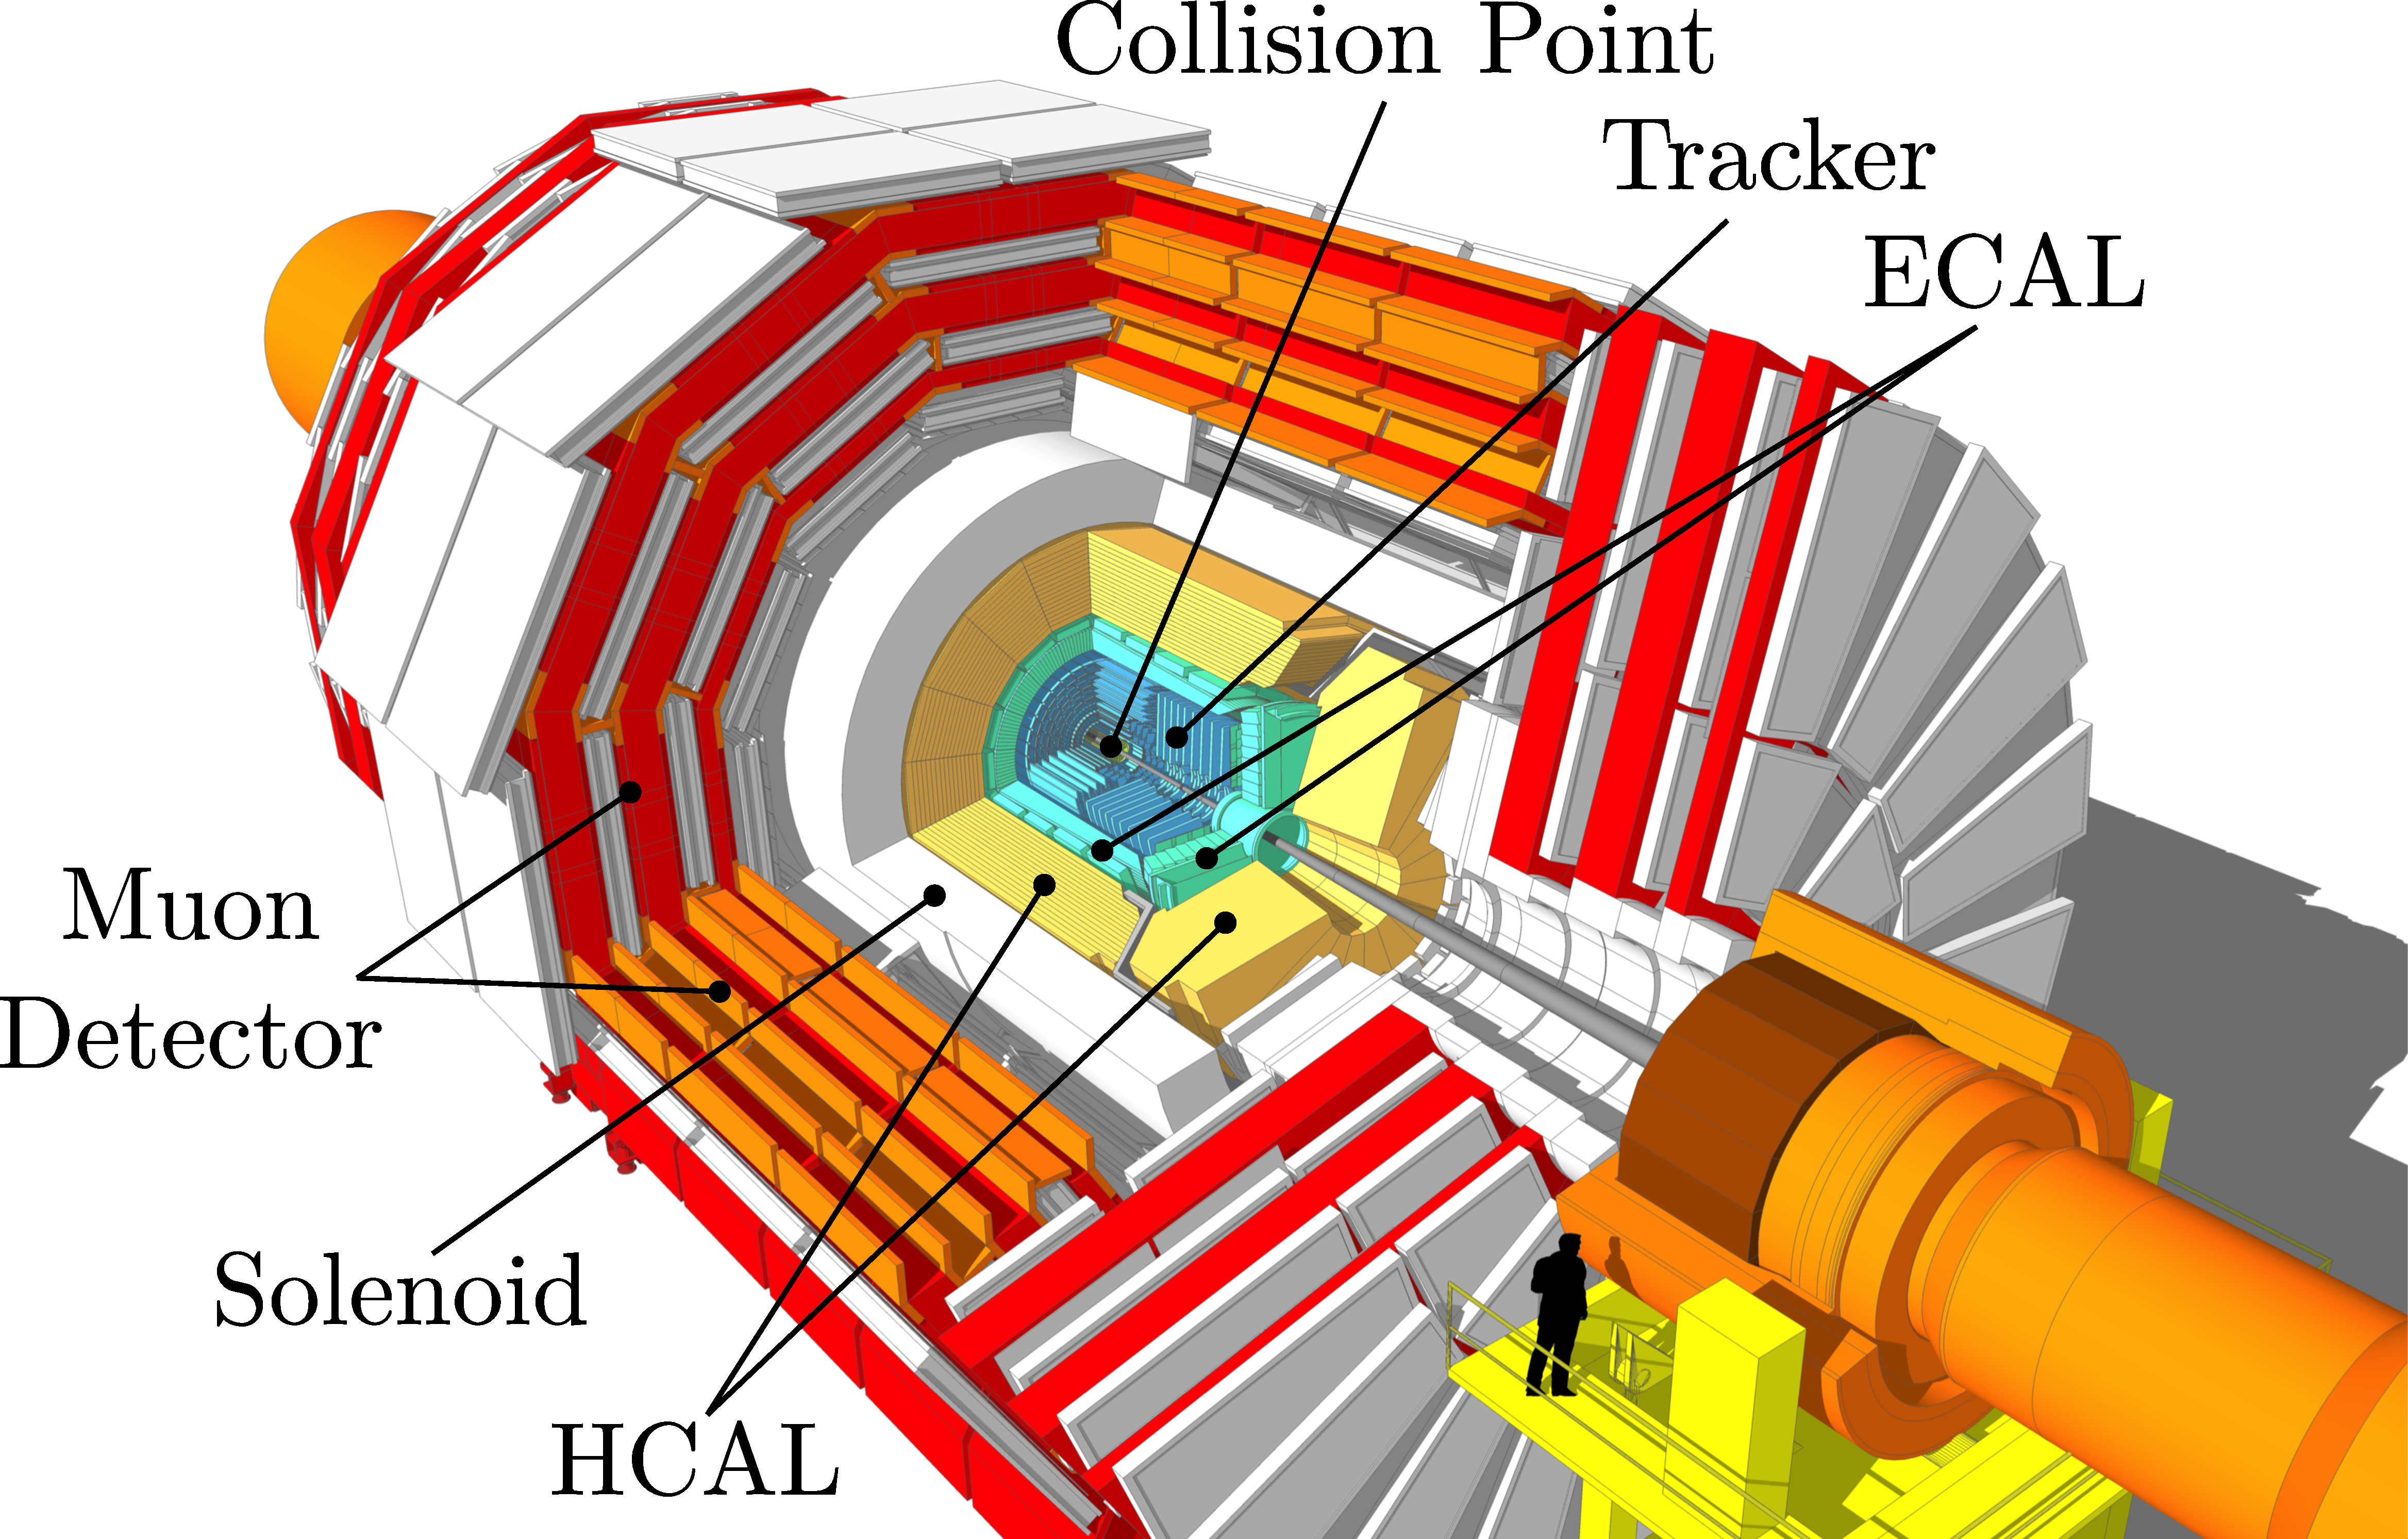
\includegraphics[width=\linewidth]{raster/raster-svg/cms-annotated.pdf}
    \end{figure}
    \vspace{-5mm}
    \tiny{Adapted from \cite{image-cms}}
    
\end{frame}

\begin{frame}
    \frametitle{The CMS Coordinate System I}
    \vspace{-3mm}
    \begin{figure}[htb!]
        \centering
        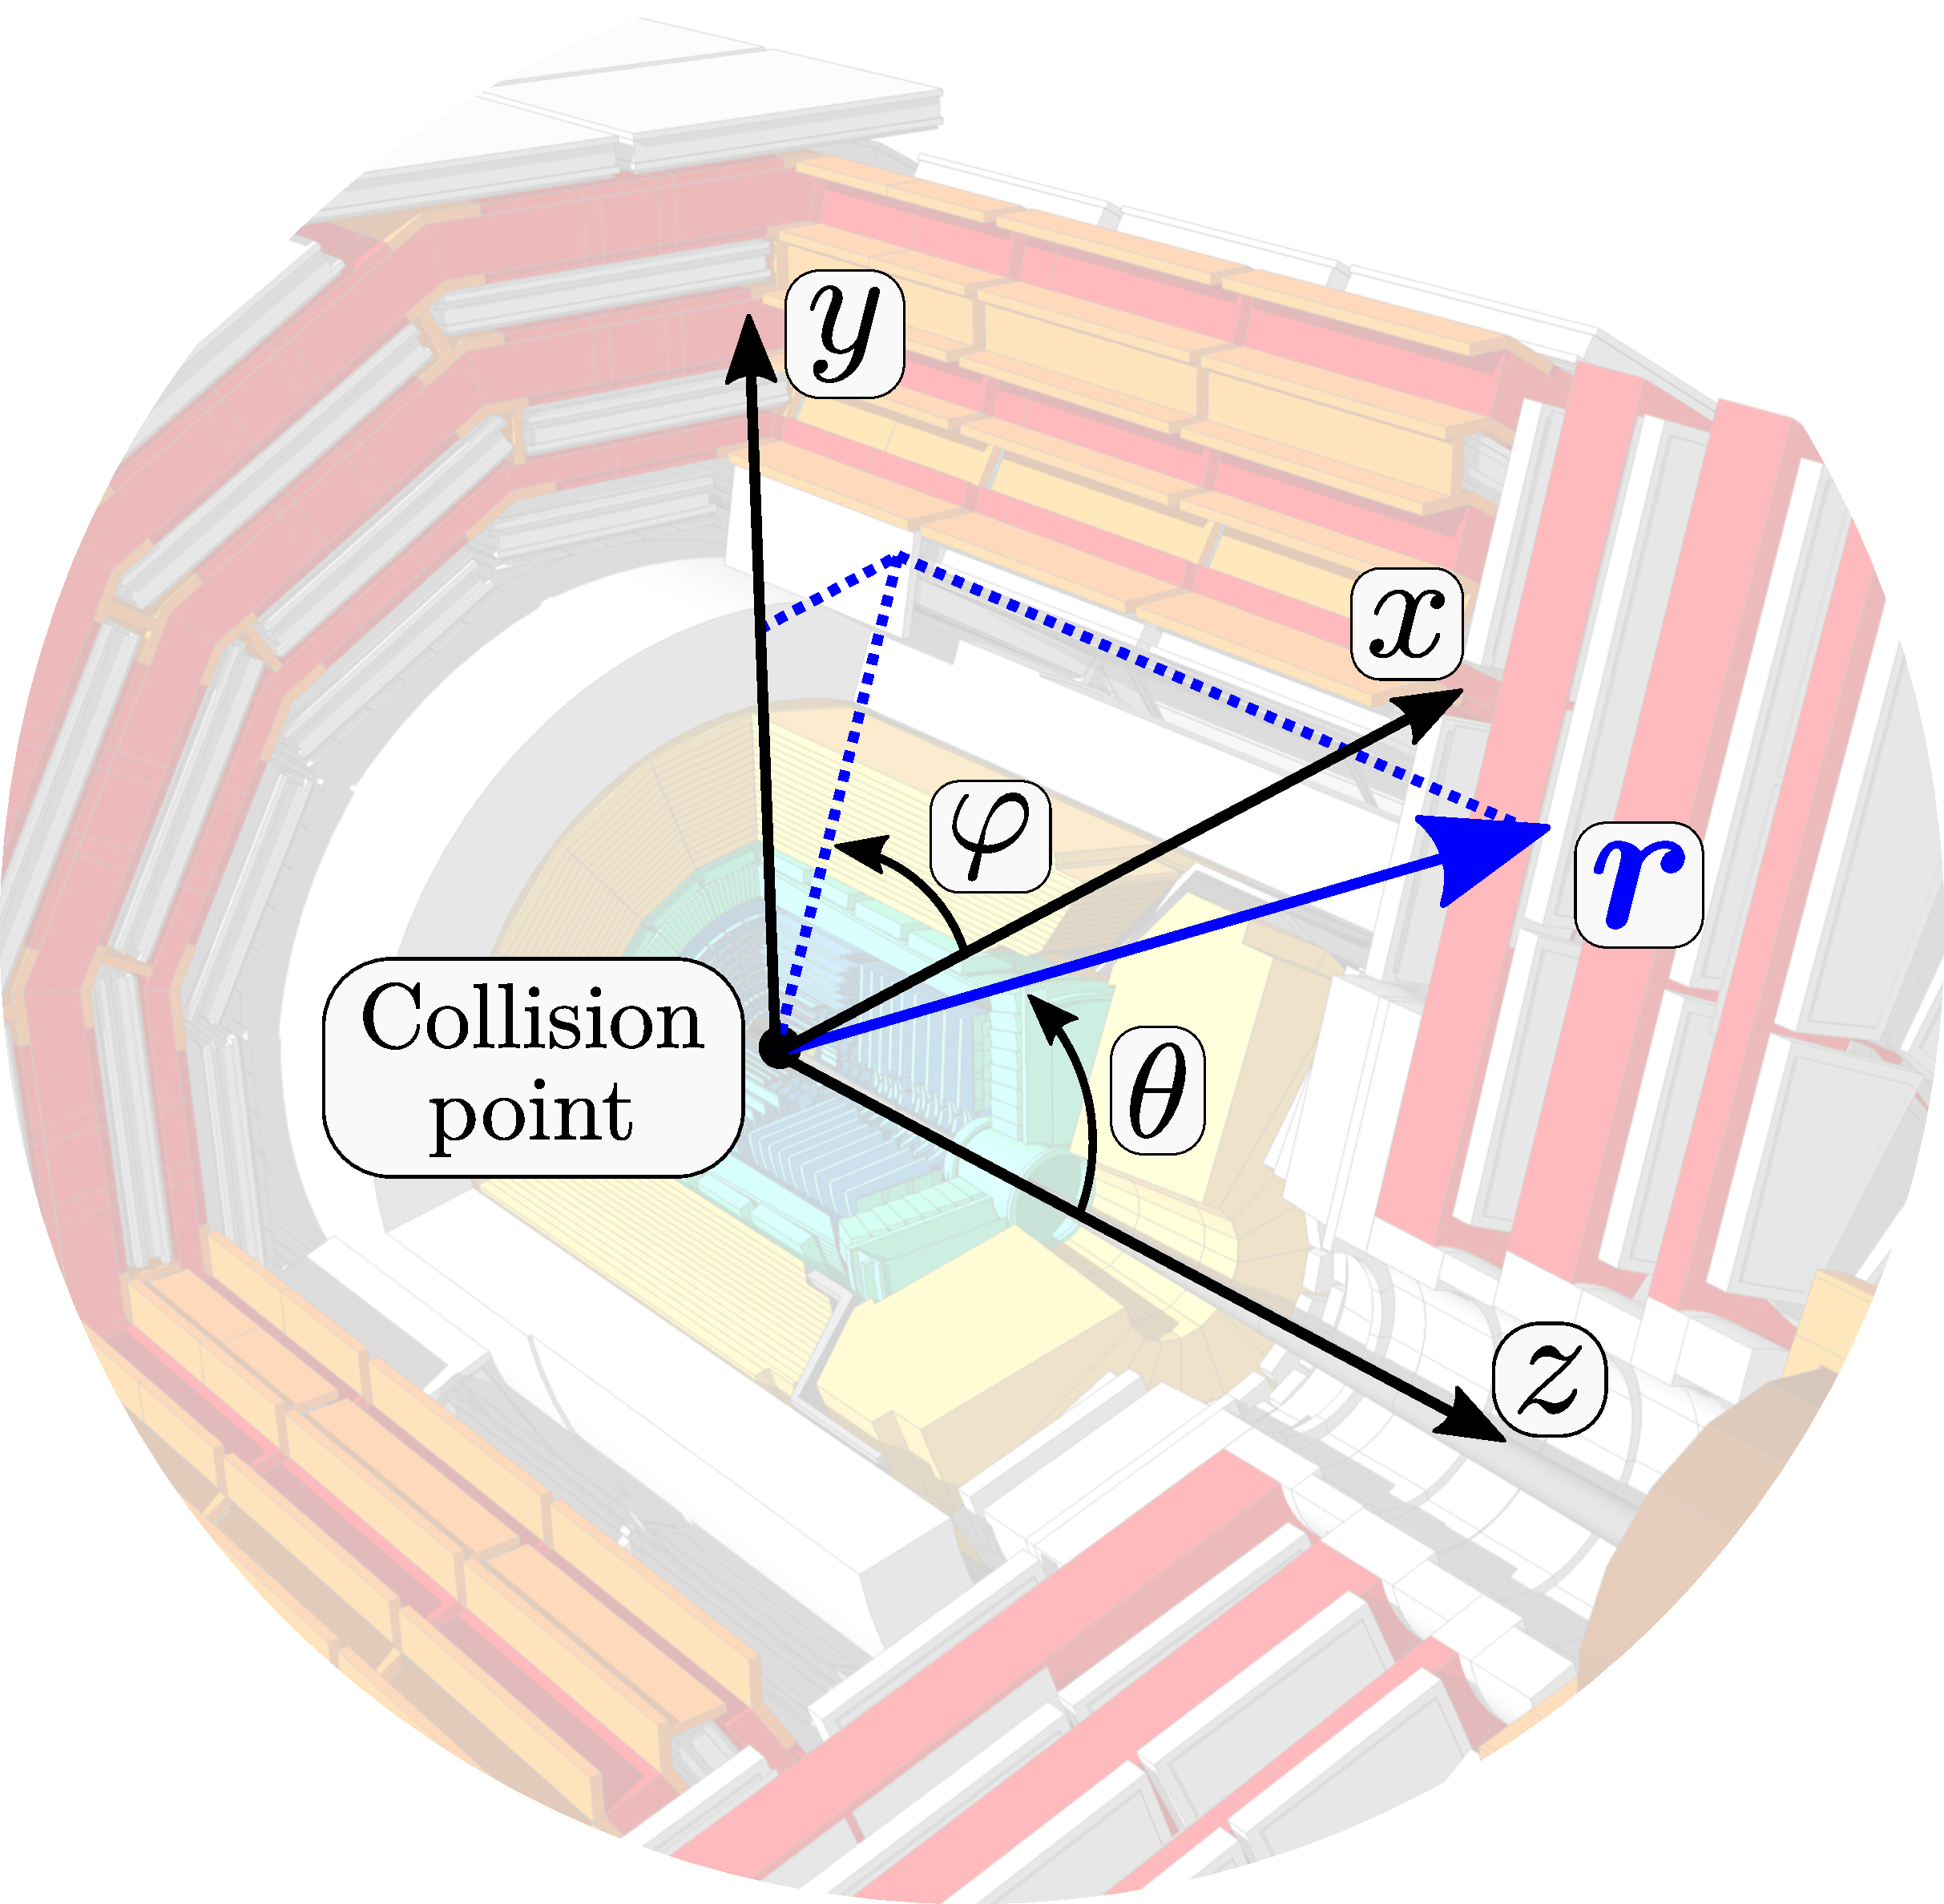
\includegraphics[width=0.85\linewidth]{raster/raster-svg/cms-coordinate.pdf}
    \end{figure}
    
\end{frame}

\begin{frame}
    \frametitle{The CMS Coordinate System II}

    \textit{Pseudorapidity} $ \eta $ preferred over $ \theta $\\
    \null \quad $ \displaystyle{\eta \equiv - \ln \left( \tan \frac{\theta}{2} \right) \implies \theta = 2 \arctan e^{- \eta}} $
    \vspace{-6mm}
    \begin{figure}[htb!]
        \centering
        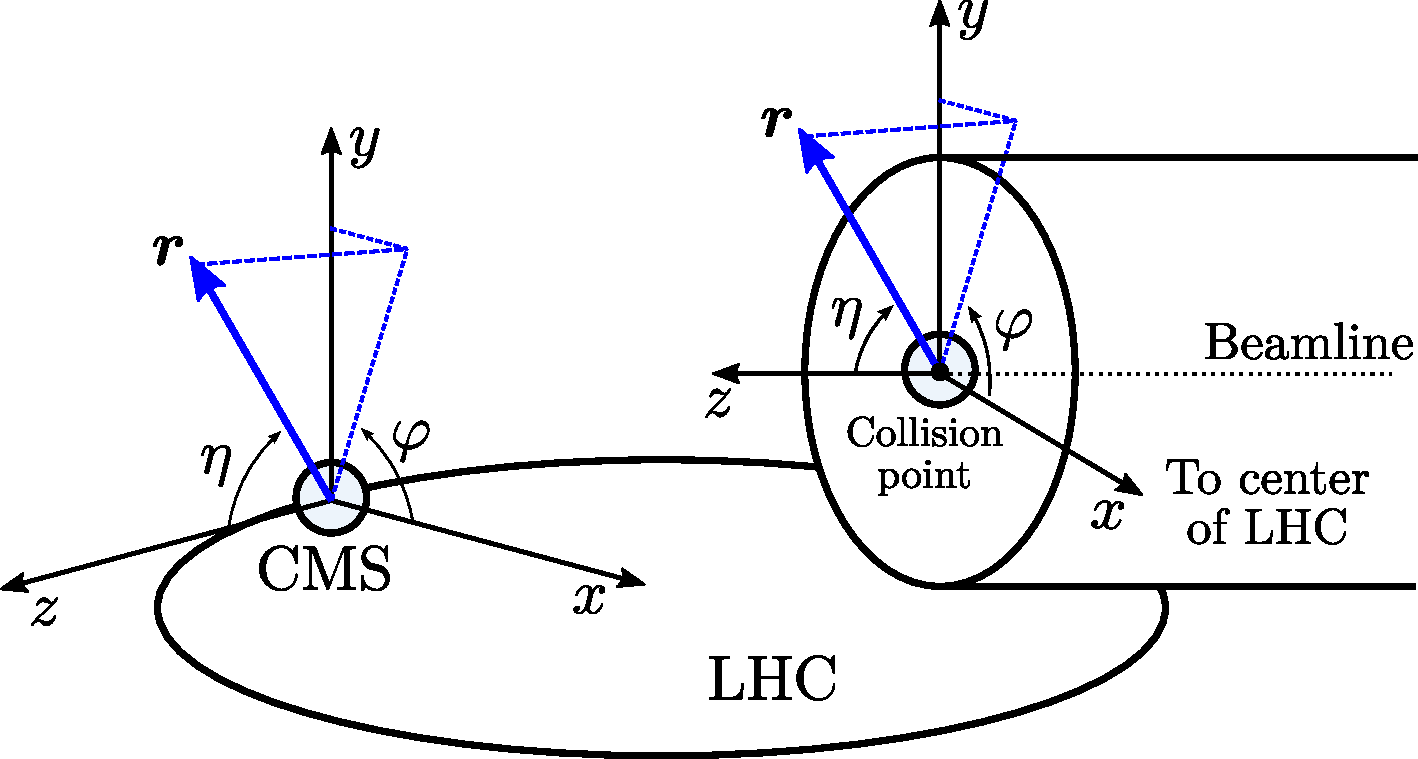
\includegraphics[width=0.9\linewidth]{vector/figures-presentation/cms-coordinate-system.pdf}
    \end{figure}
    
\end{frame}

\begin{frame}
   \frametitle{Tracker: Measuring Trajectory}
    
    Working Principle
    \begin{itemize}

     	\item Reverse-biased semiconductor\\
        \item Charged particle frees electron-hole pair\\
        \item Electron-hole pair registered as charge pulse

    \end{itemize}
    \vspace{5mm}

    \pause
    For orientation...
    \begin{itemize}
    
        \item 13 concentric layers of silicon pixels and strips 

        \item Dimensions $ \sim \text{\SIrange{10}{100}{\micro \meter}} $

        \item $ \sim $ 75 million read-out channels

    \end{itemize}
    
\end{frame}

\begin{frame}
    \frametitle{Electromagnetic Calorimeter (ECAL)}
    \begin{itemize}
    
        \item Measures energy of electromagnetically interacting particles

        \item Lead tungstate (\chem{PbWO_4}) scintillator crystals
        \item Dimensions $ \sim \SI{2}{\centi \meter} \times \SI{2}{\centi \meter} \times \SI{20}{\centi \meter} $

        \item $ \sim $ 75\,000 total scintillator crystals
    
    \end{itemize}
    \vspace{-3mm}
    \begin{figure}
        \centering
        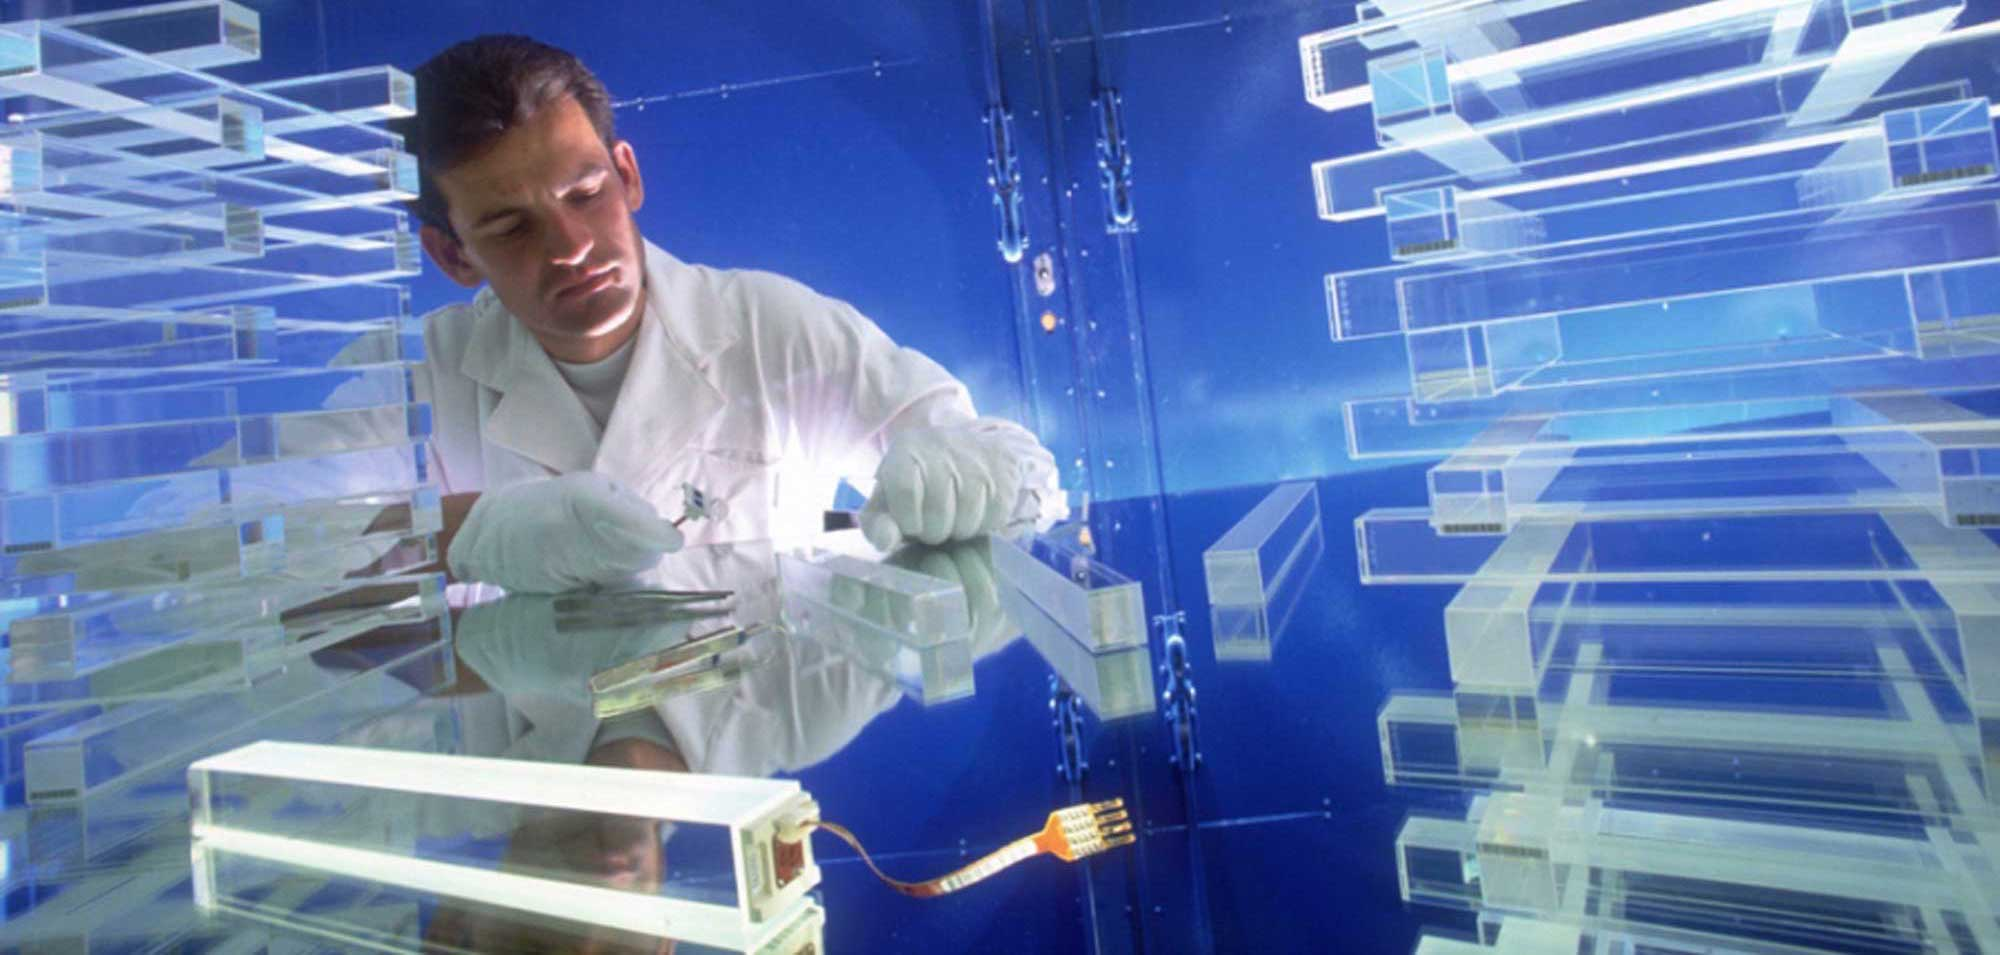
\includegraphics[width=0.75\linewidth]{raster/png-presentation/ecal-scintillators.jpg}
    \end{figure}
    \vspace{-7mm}
    \hfill
    \tiny{Source: \cite{image-pbwo4}}
    
\end{frame}

\begin{frame}
    \frametitle{ECAL Working Principle}
    \begin{itemize}
    
        \item Incident particle produces \textit{electromagnetic shower}

        \item Electromagnetic shower excites (\chem{PbWO_4}) scintillator 

        \item Scintillator emits \textit{scintillation photons}

        \item Photons free \textit{photoelectrons} in reverse-biased semiconducting photodetector

        \item Photodetector registers photoelectrons as electric signal
    
    \end{itemize}
    \begin{equation*}
        U_{0} \propto N_{e^{-}}  \propto N_{\gamma} \propto E_{\text{dep}}
    \end{equation*}
    
\end{frame}

\begin{frame}
    \frametitle{Hadronic Calorimeter (HCAL)}
    \begin{itemize}
    
        \item Measures energy of hadronic particles

        \item Brass absorbers and plastic scintillators

        \item Working principles similar to ECAL

    \end{itemize}
    
\end{frame}

\begin{frame}
    \frametitle{Detector-Data I}

    \begin{figure}[htb!]
        \centering
        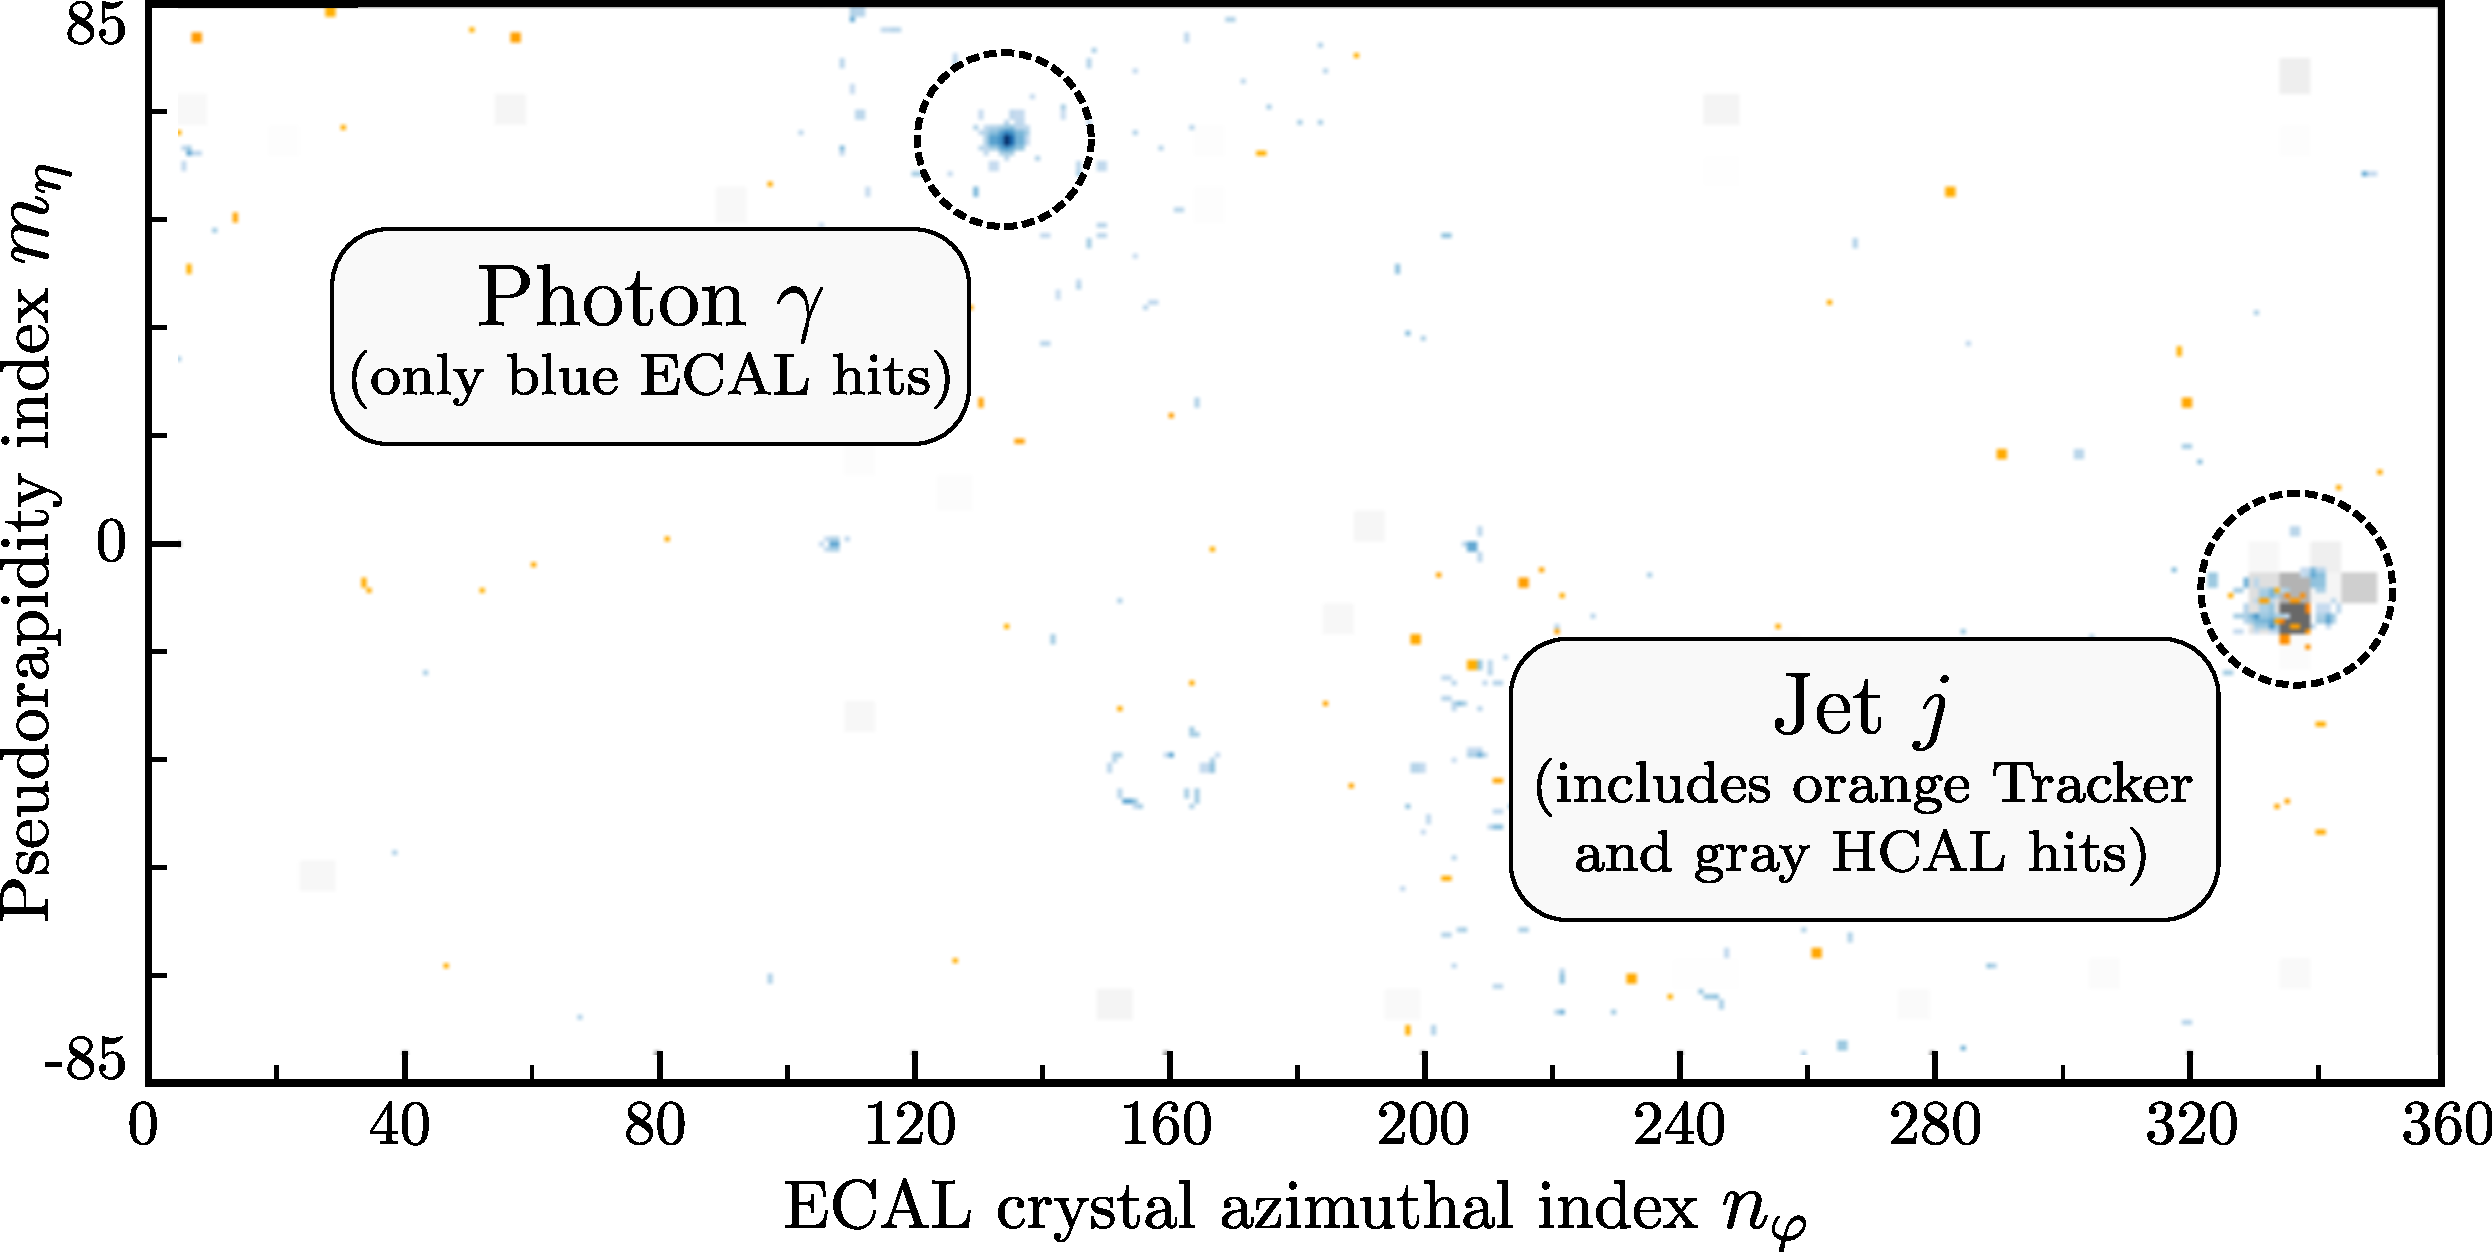
\includegraphics[width=\linewidth]{raster/raster-svg/event-image.pdf}
    \end{figure}
    \vspace{-9mm}
    \hfill
    {\tiny Adapted from \cite{andrews-higgs}}

    \vspace{-1mm}
    \begin{itemize}
    
        \item image-like pixel grid
        \item 2 spatial dimensions $ (\phi, \eta) $
        \item 3 detector channels (Tracker, ECAL, HCAL)
    
    \end{itemize}

\end{frame}

\begin{frame}
    \frametitle{Detector-Data II}
    \begin{center}
        \textit{There is a direct physical correspondence between pixel values and particle position and energy}
    \end{center}

    \vspace{-10mm}

    \begin{alignat*}{3}
        & \text{pixel intensity} && \iff &&
        \begin{cases}
            \text{charge in Tracker} &\\
            \text{energy in ECAL/HCAL} &
        \end{cases}\\[2mm]
        & \text{pixel position} && \iff && \ \text{position of...}
        \begin{cases}
            \text{silicon pixel} &\\
            \text{ECAL crystal} &\\
            \text{HCAL tile} &
        \end{cases}
    \end{alignat*}
    
    
\end{frame}

\begin{frame}
    \frametitle{Classification Options}
    \begin{enumerate}[(a)]
        \setlength{\itemsep}{5mm}
        \item \label{item:end-end} {\large \underline{End-to-end classification}}: directly use image-based detector data

        \item \label{item:kinematic}
        {\large \underline{Kinematic-based classification}}: first reconstruct kinematic features

        \item \label{item:high-level} {\large \underline{High-level classification}}: first reconstruct kinematic features, then hand-engineer custom \textit{high-level} features
    
    \end{enumerate}
    We will call (\ref{item:kinematic}) and (\ref{item:high-level}) \textit{traditional classification}.
    
\end{frame}

\section{Traditional Classification}

\begin{frame}
    \frametitle{Traditional Classification}
    \begin{enumerate}[(a)]
    
        \item Training
        \begin{itemize}
        
            \item \textit{Simulate} collision data ($ \sim 10^{6} $ collisions)

            \item Train neural network with simulated data
        
        \end{itemize}
        \pause
        \vspace{1mm}
        \begin{center}
        \begin{figure}[htb!]
            \hspace{-10mm} % hack to center figure with slide and not itemize environment
            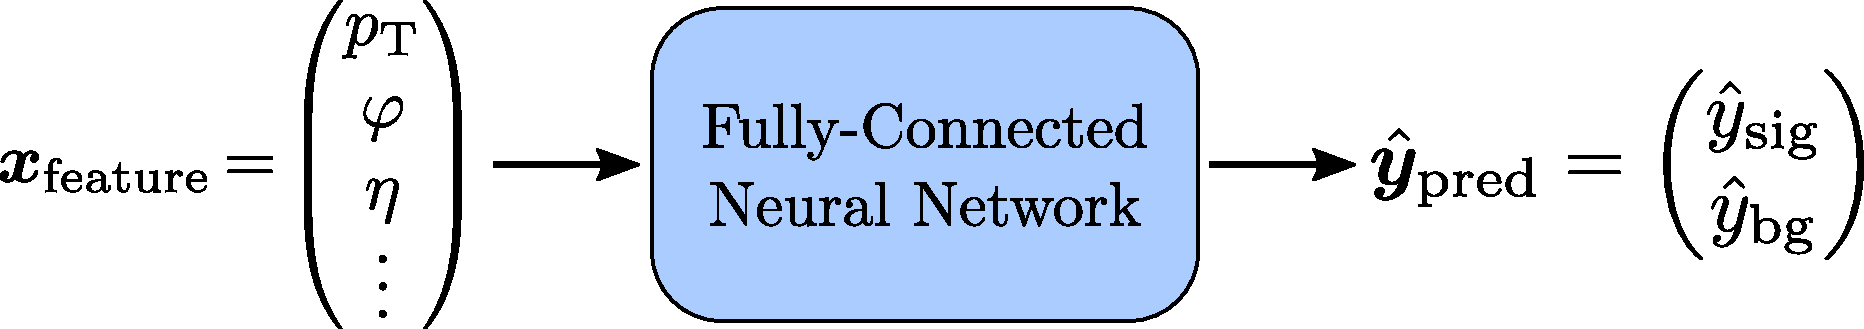
\includegraphics[width=\linewidth]{vector/fcn-in-out.pdf}
        \end{figure}    
        \end{center}
        
        \item Application
        \begin{itemize}
        
            \item Reconstruct kinematic quantities describing each LHC collision ($ \vec{x}_{\text{feature}} $)

            \item Pass quantities into fully-connected network

            \item Output classification result
        
        \end{itemize}
    
    \end{enumerate}
       
\end{frame}

\begin{frame}
    \frametitle{Understanding a Classifier's Output}
    \begin{itemize}
    
        \item True result:
        $ \vec{y} = 
        \begin{pmatrix}
            y_{\text{sig}}\\[-0.5mm]
            y_{\text{bg}}
        \end{pmatrix} $ \ {\small (known from simulation)}

        \item Prediction: \hspace{-1.0mm}
        $ \hat{\y} = 
        \begin{pmatrix}
            \hat{y}_{\text{sig}}\\[-0.5mm]
            \hat{y}_{\text{bg}}
        \end{pmatrix} $

        \item Classes represented by binary 1/0 values
        
    \end{itemize}
    
    \begin{figure}[htb!]
        \centering
        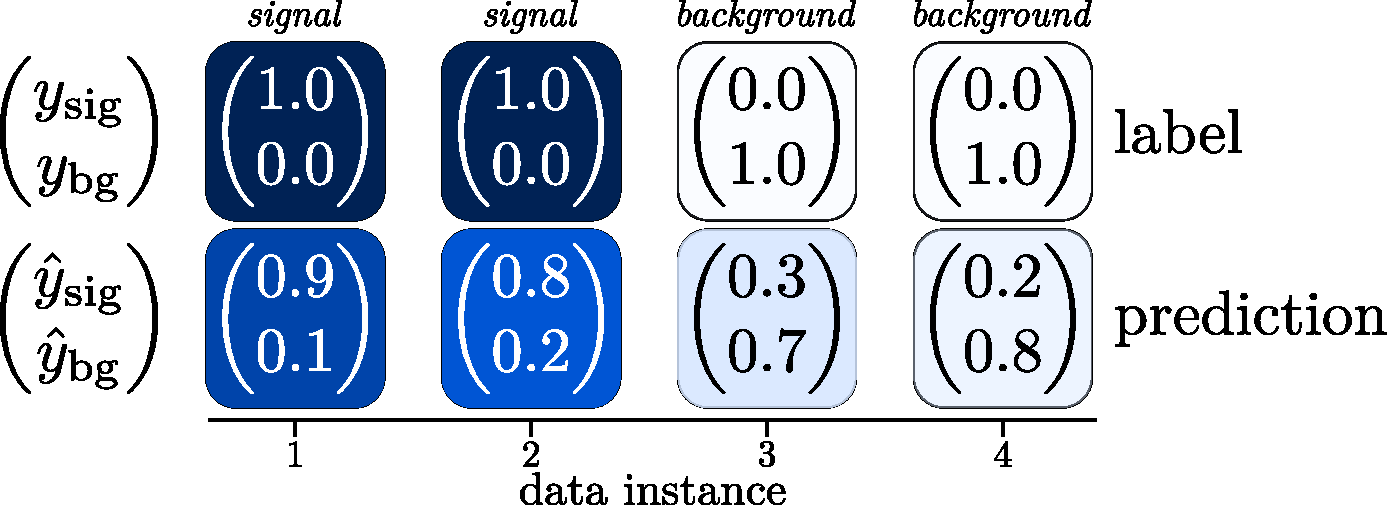
\includegraphics[width=\linewidth]{vector/binary-output.pdf}
    \end{figure}
    
\end{frame}

% Note to self: ``The notation $ \y $ will be consistent throughout this presentation to denote predicted classification scores!''

\begin{frame}
    \frametitle{Anatomy of a Fully-Connected Network}

    \begin{itemize}
    
        \item<1-> Hierarchy: {\small (i) neuron} \ (ii) layer \ {\large (iii) network}

        \item<2-> Input layer: collision information enters
                  
        \item<3-> Hidden layers: calculations
                  
        \item<4-> Output layer: classification scores
    
    \end{itemize}
    \vspace{-4mm}
    \begin{figure}[htb!]
        \centering
        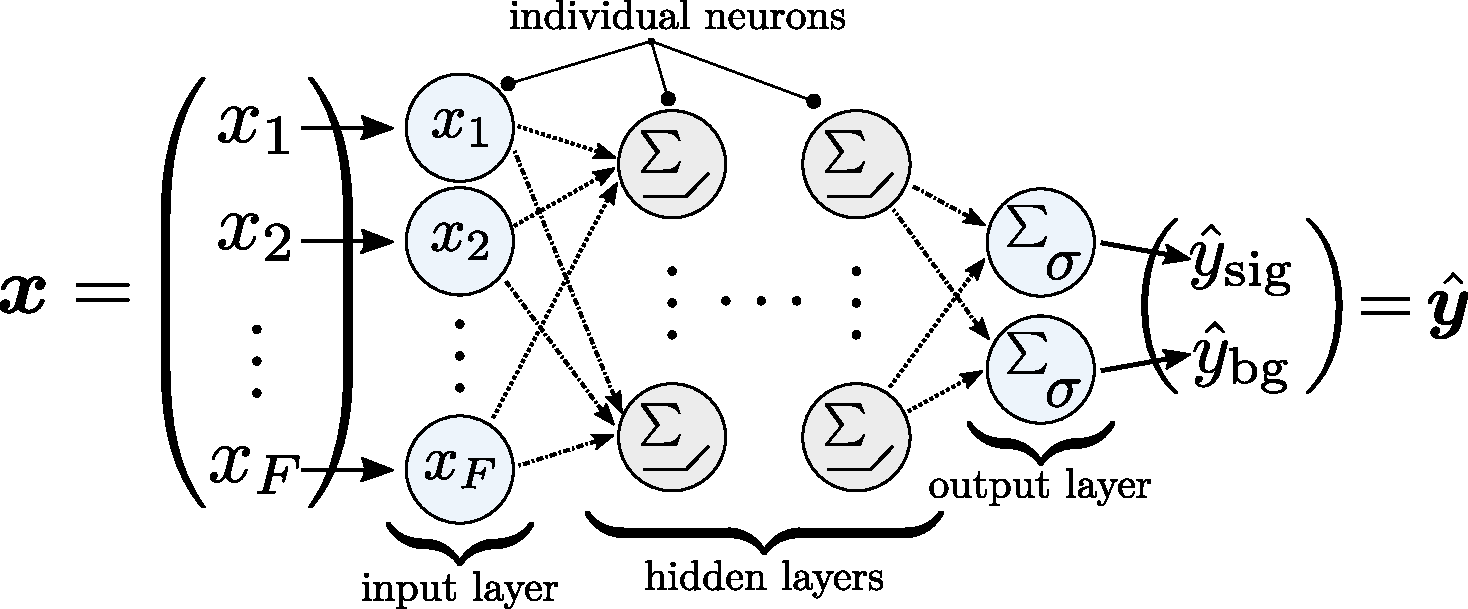
\includegraphics[width=\linewidth]{vector/fcn-architecture-simple.pdf}
    \end{figure}
\end{frame}

\begin{frame}
    \frametitle{A Single Neuron}
    \begin{itemize}
    
        \item Essentially a multi-variable scalar function

        \item Input: output of all neurons in previous layer

        \item Output: a scalar \textit{activation value} $ {\color{myMaroon} a} \in \mathbb{R} $
    
    \end{itemize}
    \onslide<2->{Two steps:
    \begin{enumerate}[(i)]
    
        \item \textit{linear} weighted sum $ z = \w \cdot \a_{\text{prev}} + b $


        \item \textit{non-linear} activation $ {\color{myMaroon} a} = f_{\text{a}}(z) $
    
    \end{enumerate}}

    
    \begin{columns}
        \column{0.6\textwidth}
        \vspace{-8mm}
        \begin{figure}
            \centering
            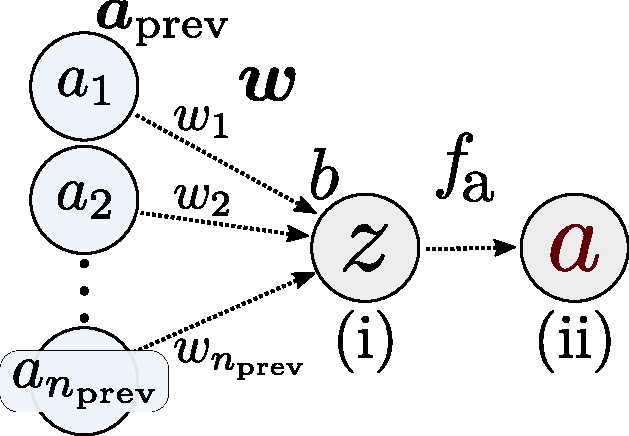
\includegraphics[width=0.8\columnwidth]{vector/figures-presentation/fcn-single-neuron}
        \end{figure}

        \column{0.4\textwidth}
        \onslide<2->{
        \begin{alignat*}{3}
            \text{(i)}& \ && z \mspace{-2mu} &&= \mspace{-2mu} \bm{w} \mspace{-3mu} \cdot \mspace{-3mu} \bm{a}_{\text{prev}} \mspace{-2mu} + \mspace{-2mu} b \in \mathbb{R} \\[-0.5mm]
            \text{(ii)}& \ && {\color{myMaroon} a} \mspace{-3mu} && = \mspace{-4mu} f_{\raisebox{-0.2ex}{\scalebox{0.9}{$\mspace{-2mu} \mathrm{a}$}}}(z) \in \mathbb{R}
        \end{alignat*}}
        
    \end{columns}

\end{frame}

\begin{frame}
    \frametitle{Activation Function}

    \textit{Non-linear} function of pre-activation value
    \begin{equation*}
        a = f_{\text{a}}(z) = f_{\text{a}} \big(\mspace{-2mu} \bm{w} \mspace{-3mu} \cdot \mspace{-3mu} \bm{a}_{\text{prev}} \mspace{-2mu} + \mspace{-2mu} b \big) \in \mathbb{R}
    \end{equation*}
    
    \only<1>{
        \vspace{-2mm}
        \begin{center}
            \textit{Non-linear activation functions allow non-linear decision boundaries!}    
        \end{center}
        \vspace{-1mm}
        \begin{figure}
            \centering
            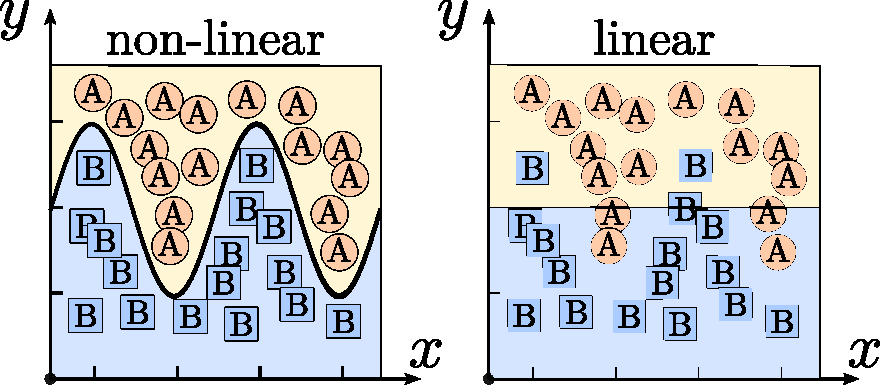
\includegraphics[width=\linewidth]{vector/figures-presentation/decision-boundary}
        \end{figure}
    }

    \only<2>{
        \vspace{-6mm}
        \begin{columns}
            \column{0.57\linewidth}
            \vspace{3mm}
            \begin{itemize}
            
                \item Common functions: $ \mathrm{ReLU} $ and variants, sigmoid, $ \tanh $, etc...

                \item (Generally) continuously differentiable

                \item ReLU common in CNNs

            \end{itemize}
            \column{0.55\linewidth}
            \begin{figure}[htb!]
                \centering
                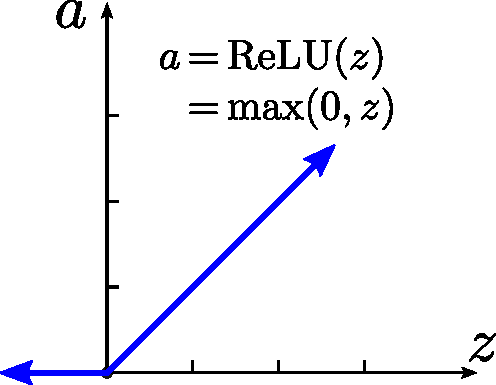
\includegraphics[width=\columnwidth]{vector/relu.pdf}
            \end{figure}
        \end{columns}}
    
    
\end{frame}

\begin{frame}
    \frametitle{A Network Layer}

    \begin{itemize}
    
        \item Weight vectors $ \w $ $ \longrightarrow $ weight matrix $ \W $

        \item Biases $ b $ $ \longrightarrow $ bias vector $ \b $
        \item Activation $ a $ $ \longrightarrow $ activation vector $ {\color{myMaroon} \a} $
    
    \end{itemize}
    
    \onslide<2->{Two steps:
    \begin{enumerate}[(i)]
    
        \item \textit{linear} affine transformation $ \z \mspace{-2mu} = \mspace{-2mu} \W^{\top} \mspace{-6mu} \cdot \mspace{-2mu} \bm{a}_{\text{prev}} \mspace{-2mu} + \mspace{-2mu} \b $


        \item \textit{non-linear} activation $ {\color{myMaroon} \a} = f_{\text{a}}(\z) $
    
    \end{enumerate}}

    \begin{columns}
        \column{0.6\textwidth}
        \vspace{-8mm}
        \begin{figure}
            \centering
            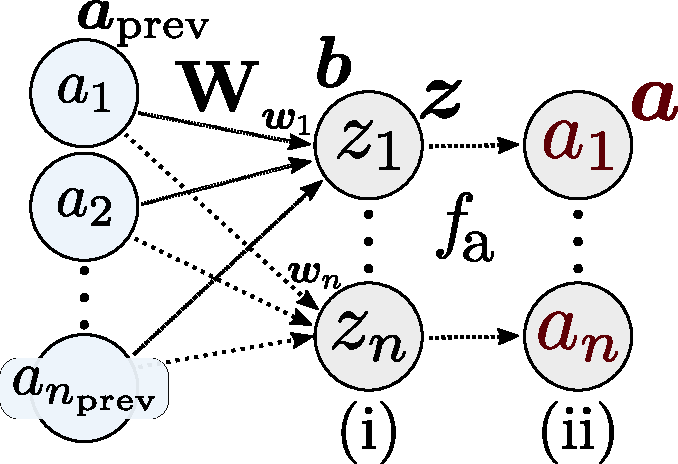
\includegraphics[width=0.8\columnwidth]{vector/figures-presentation/fcn-single-layer}
        \end{figure}

        \column{0.4\textwidth}
        \onslide<2->{
        \begin{alignat*}{3}
            \text{(i)}& \ && \z \mspace{-2mu} &&= \mspace{-2mu} \W^{\top} \mspace{-6mu} \cdot \mspace{-2mu} \bm{a}_{\text{prev}} \mspace{-2mu} + \mspace{-2mu} \b \in \mathbb{R}^{n} \\[-0.5mm]
            \text{(ii)}& \ && {\color{myMaroon} \a} \mspace{-3mu} && = \mspace{-4mu} f_{\raisebox{-0.2ex}{\scalebox{0.9}{$\mspace{-2mu} \mathrm{a}$}}}(\z) \in \mathbb{R}^{n}
        \end{alignat*}}
        
    \end{columns}

\end{frame}

\begin{frame}
    \frametitle{Interpreting a FCN}

    \begin{itemize}
    
        \item $ F $ features (input) and $ C $ classes (output)

        \item Input: features $ \x \in \mathbb{R}^{F} $ and labels $ \y \in \mathbb{R}^{C} $

        \item Output: classification scores $ \hat{\y} \in \mathbb{R}^{C} $

    \end{itemize}
    \begin{center}
        \textit{A FCN is a vector function $ \vec{h}: \mathbb{R}^{F} \to \mathbb{R}^{C} $ parameterized by weights $ \W^{(l)} $ and biases $ \b^{(l)} $}
    \end{center}

    \pause
    \begin{block}{Training Goal}
        Find optimal values $ \W_{\text{opt}}^{(l)} $ and $ \b_{\text{opt}}^{(l)} $ such that prediction $ \hat{\y} = \vec{h}(\x) $ matches label $ \y $
    \end{block}
    
\end{frame}

\begin{frame}
    \frametitle{Optimization}
    \begin{itemize}
    
        \item \textit{Loss} $ L : \mathbb{R}^{C} \to \mathbb{R} $ \underline{quantifies} difference between prediction $ \hat{\y} $ and true result $ \y $

        \item Input predictions $ \hat{\y} \in \mathbb{R}^{C} $, output loss $ L \in \mathbb{R} $

        \item Example: \textit{categorical cross entropy}
        \vspace{-3mm}
        \begin{equation*}
            L(\hat{\y}; \y) = - \sum_{c = 1}^{C} y_{c} \ln \hat{y}_{c}
        \end{equation*}
    \end{itemize}
    \vspace{-5mm}
    \begin{center}
        \textit{We optimize weights and biases by minimizing loss!}
    \end{center}
    \pause
    \vspace{-3mm}
    ...using numerical methods for multi-dimensional minimization problems adapted to very large parameter spaces and huge datasets.
    
\end{frame}

\section{End-to-End Classification}

\begin{frame}
    \frametitle{End-to-End Classification}

    \vspace{2mm}
    Recall our image-based detector data...
    \only<1>{
    \begin{figure}[htb!]
        \centering
        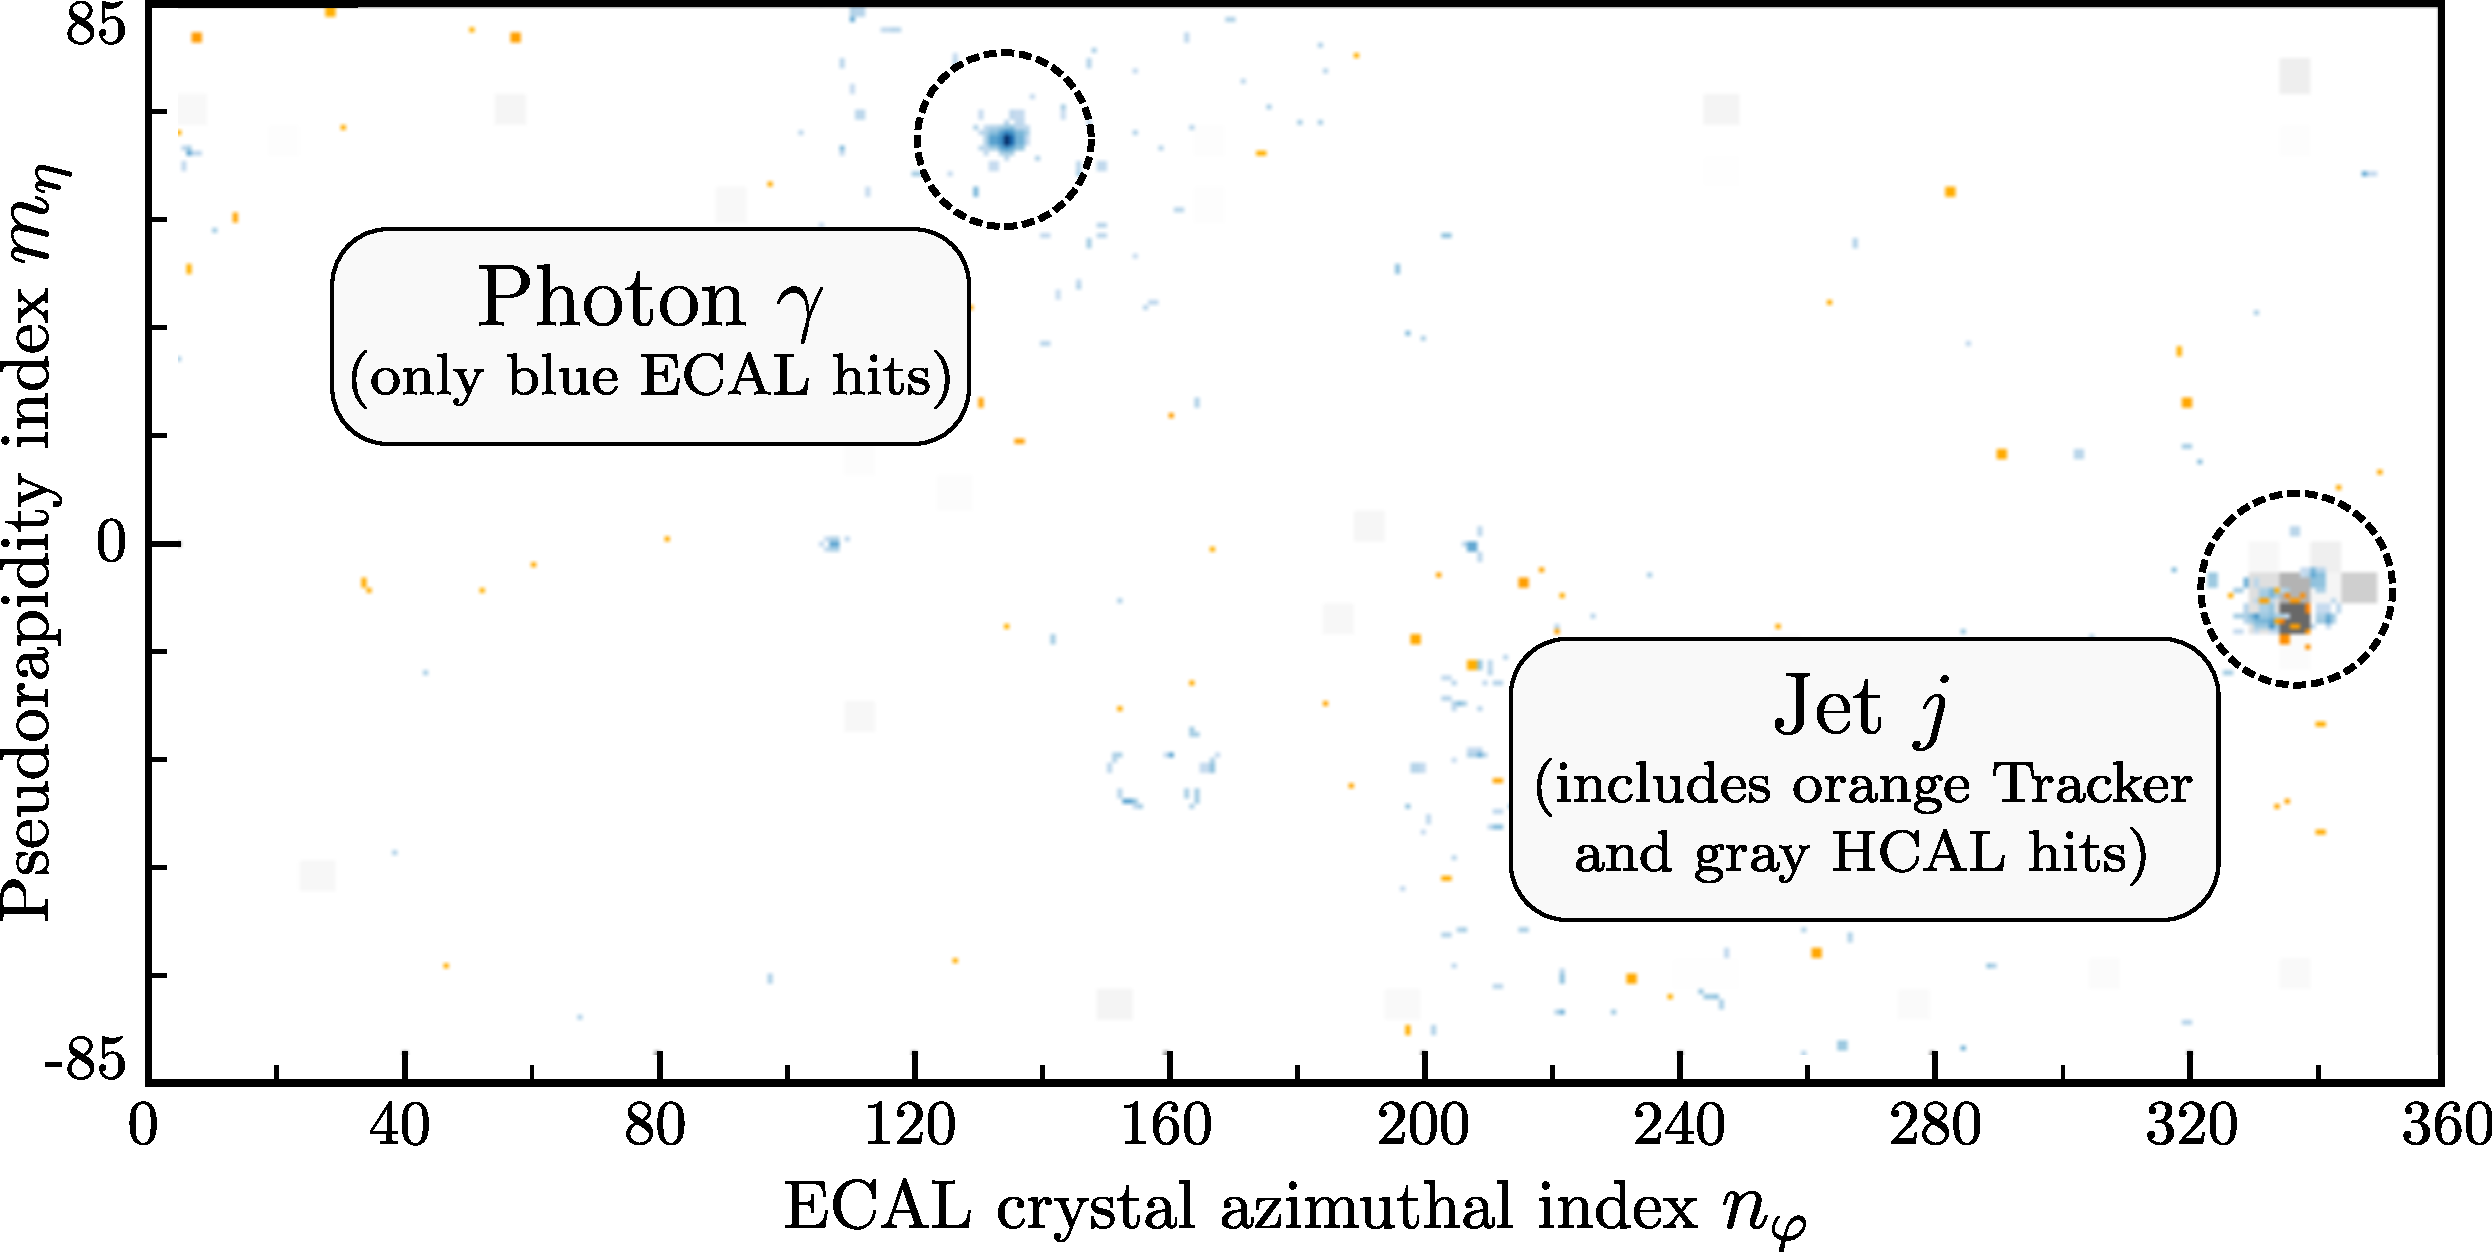
\includegraphics[width=\linewidth]{raster/raster-svg/event-image.pdf}
    \end{figure}}

    \only<2>{
    \begin{figure}[htb!]
        \centering
        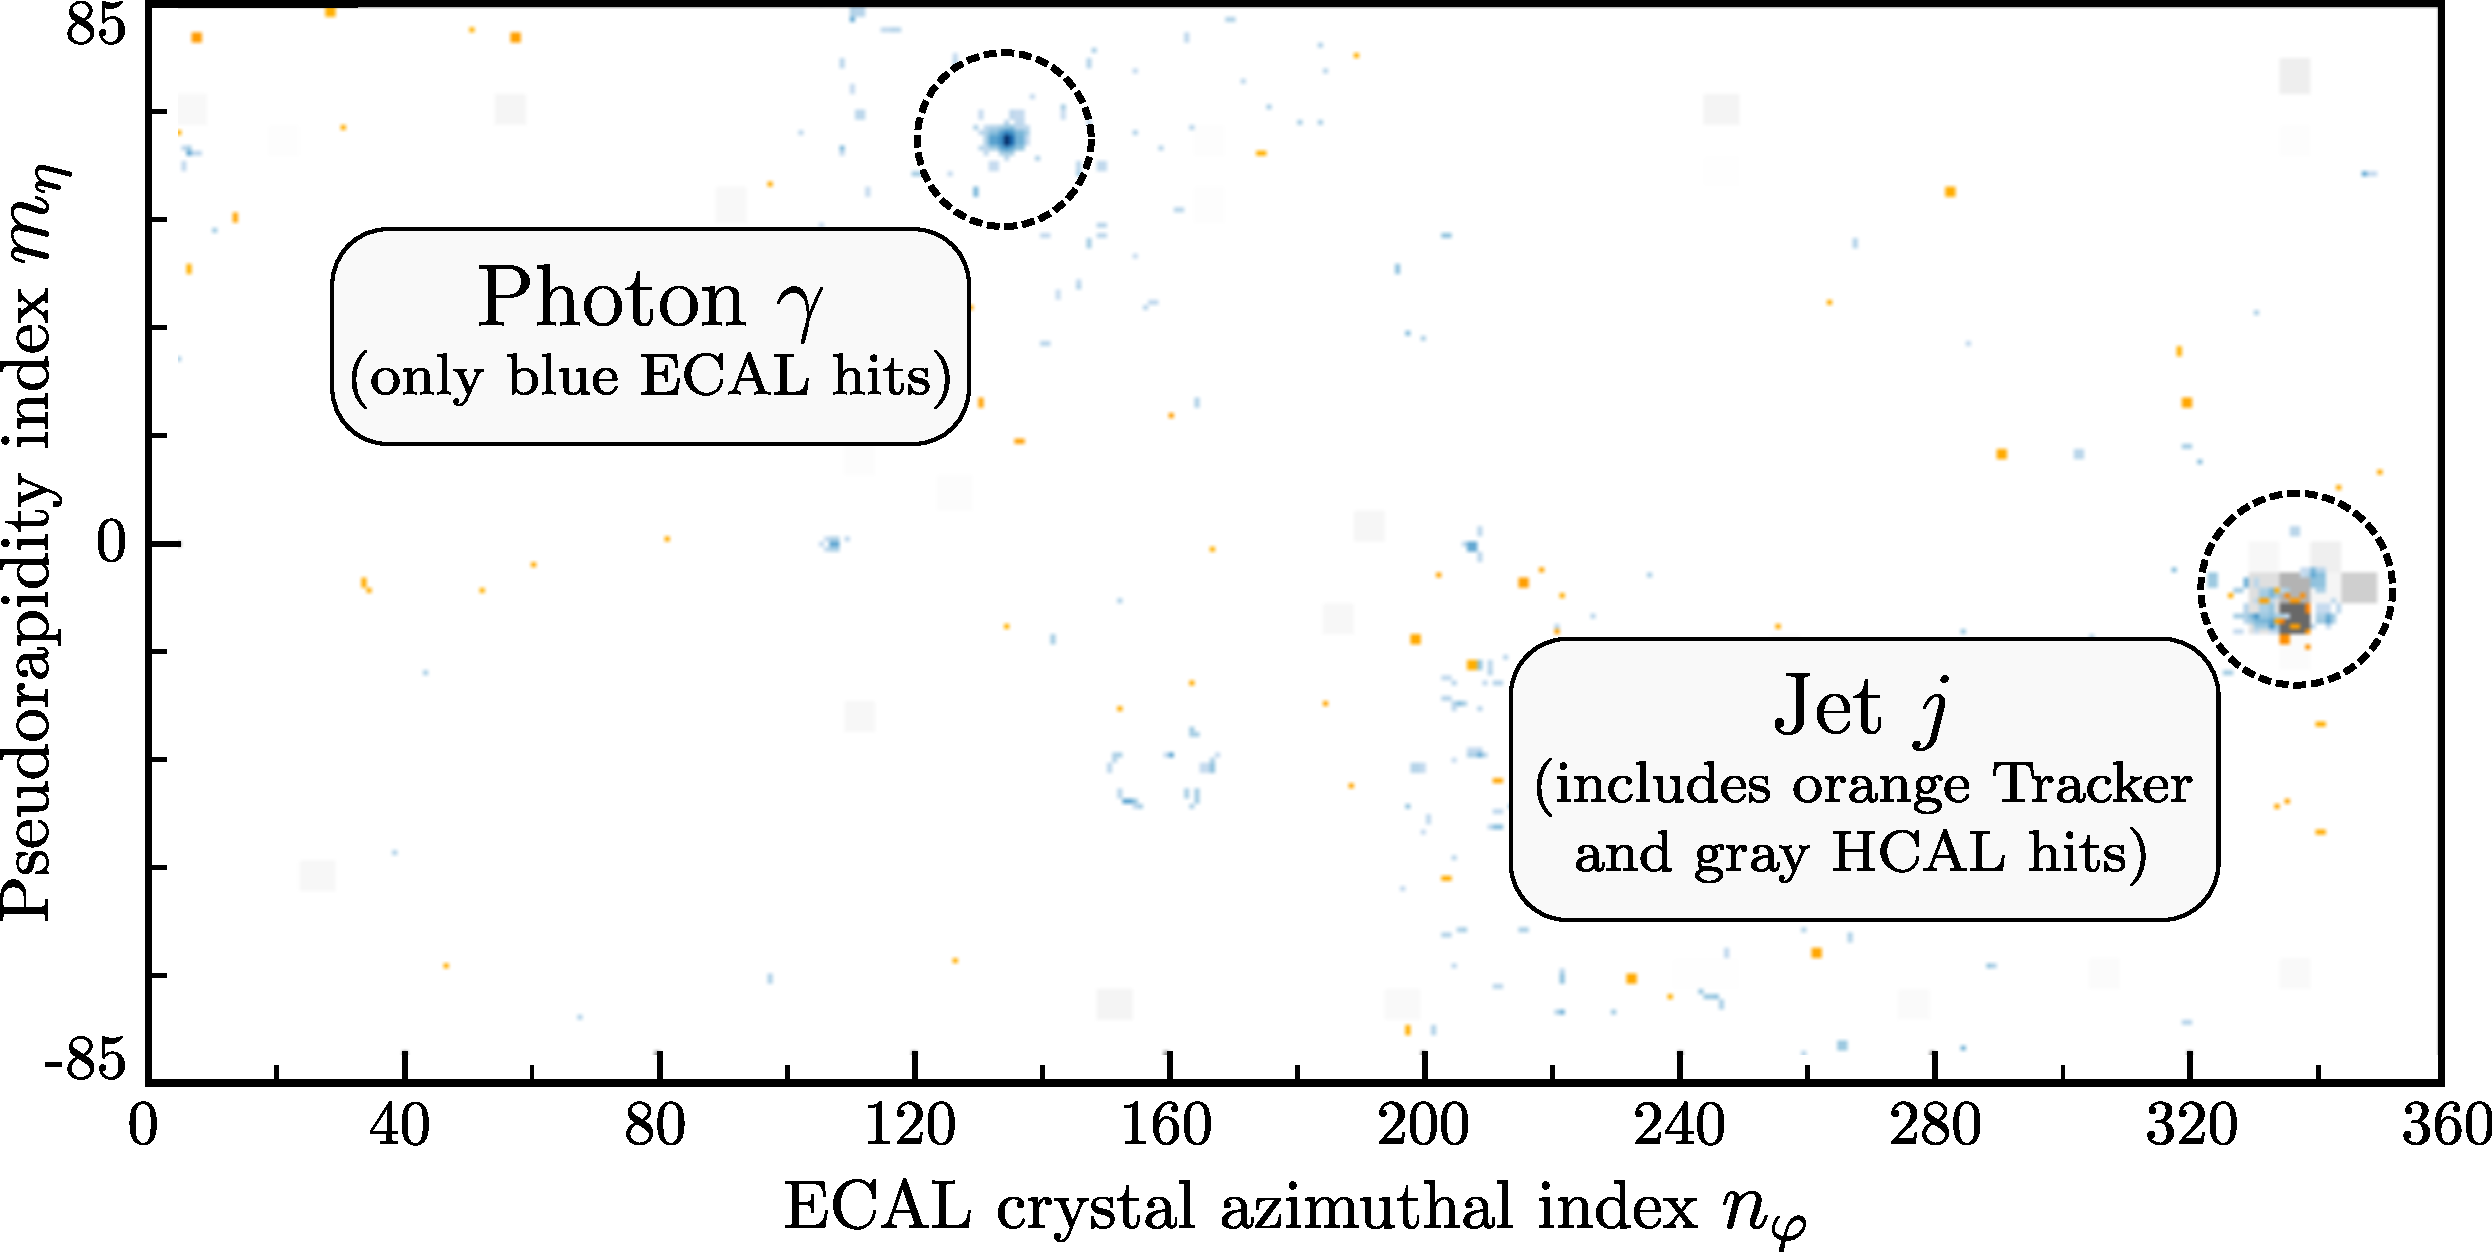
\includegraphics[width=0.7\linewidth]{raster/raster-svg/event-image.pdf}
    \end{figure}
    \vspace{-3mm}
    End-to-end classification looks like this:
    \begin{figure}[htb!]
        \centering
        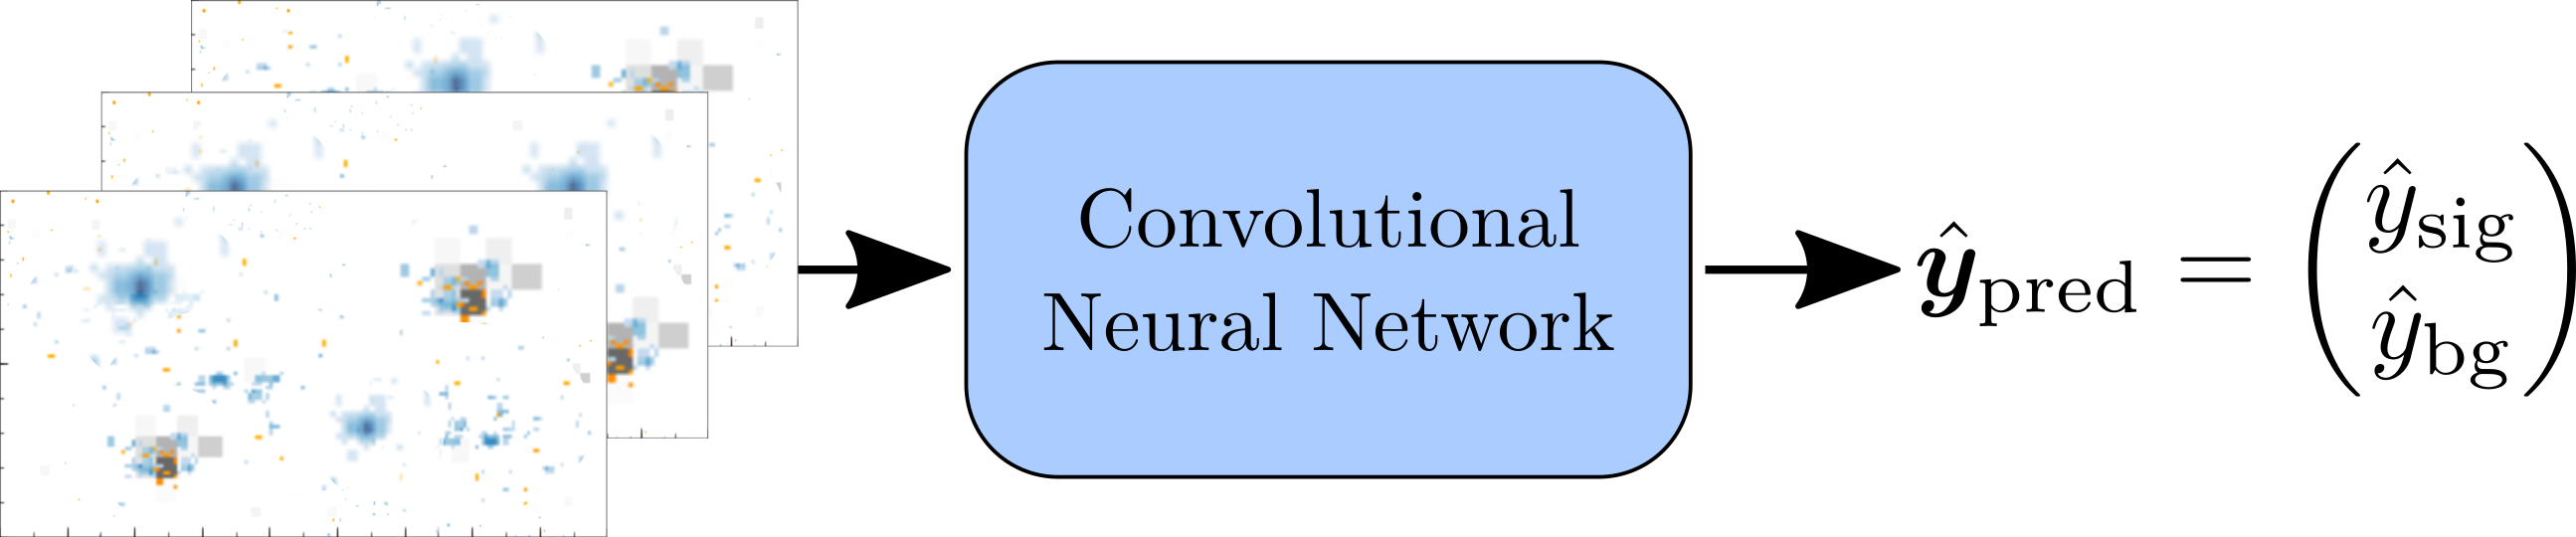
\includegraphics[width=0.9\linewidth]{raster/raster-svg/cnn-in-out.png}
    \end{figure}}
\end{frame}

\begin{frame}
    \frametitle{Motivation for Convolutional Networks}

    Let's examine the input data...
    \begin{itemize}
    
        \item stored as multi-dimensional arrays

        \item one \textit{channel axis} for different subdetectors

        \item two \textit{spatial axes} for coordinates $ \varphi $ and $ \eta $
    
    \end{itemize}
    \vspace{2mm}
    Spatial structure stores physical information!

    \begin{figure}[htb!]
        \centering
        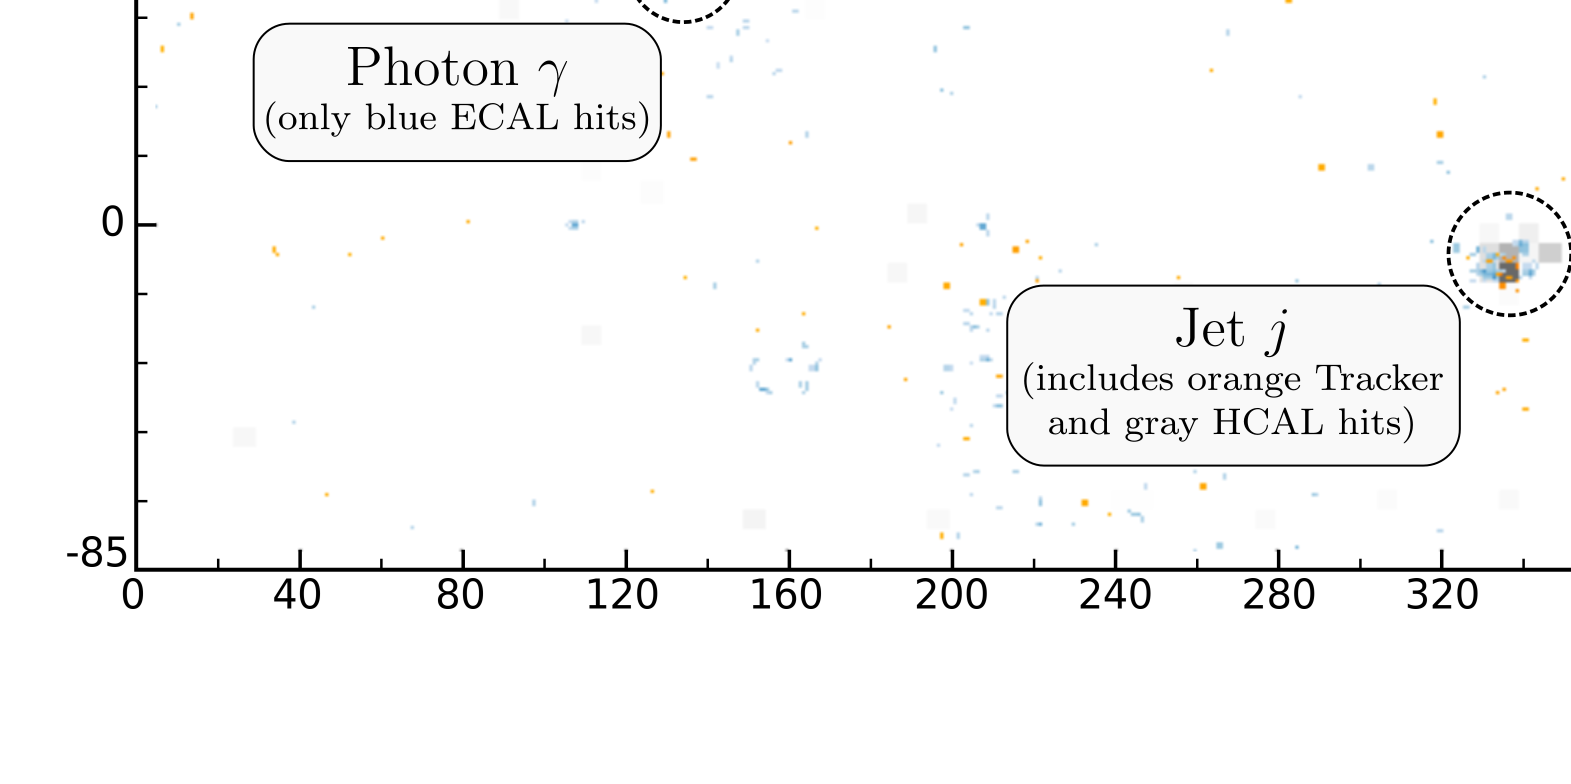
\includegraphics[width=0.85\linewidth]{raster/raster-svg/event-image-cropped}
    \end{figure}   
    
\end{frame}


\begin{frame}
    \frametitle{Motivation for Convolutional Networks II}

    \begin{block}{The Goal of Convolutional Networks}
        Preserve and leverage the information encoded in an input image’s \textit{spatial structure}
    \end{block}
    \hspace{2mm} ...in a way that FCNs, limited to flattened, \textit{one-dimensional} vector inputs, cannot.

    \pause
    \vspace{5mm}
    \begin{center}
        {\large We need a \textit{space-preserving} way for CNNs to interact with input images!}
    \end{center}
    

\end{frame}

\begin{frame}
    \frametitle{Discrete Convolution}

    \begin{itemize}
    
        \item Intuitively: ``scan'' 2D image with 2D ``filter''

        \item Mathematically: \textit{convolve} image with convolutional kernel

        \item Kernel has weights and bias (like FCN neuron)

        \item Parameters detect distinguishing features

    \end{itemize}

    \begin{figure}[htb!]
        \centering
        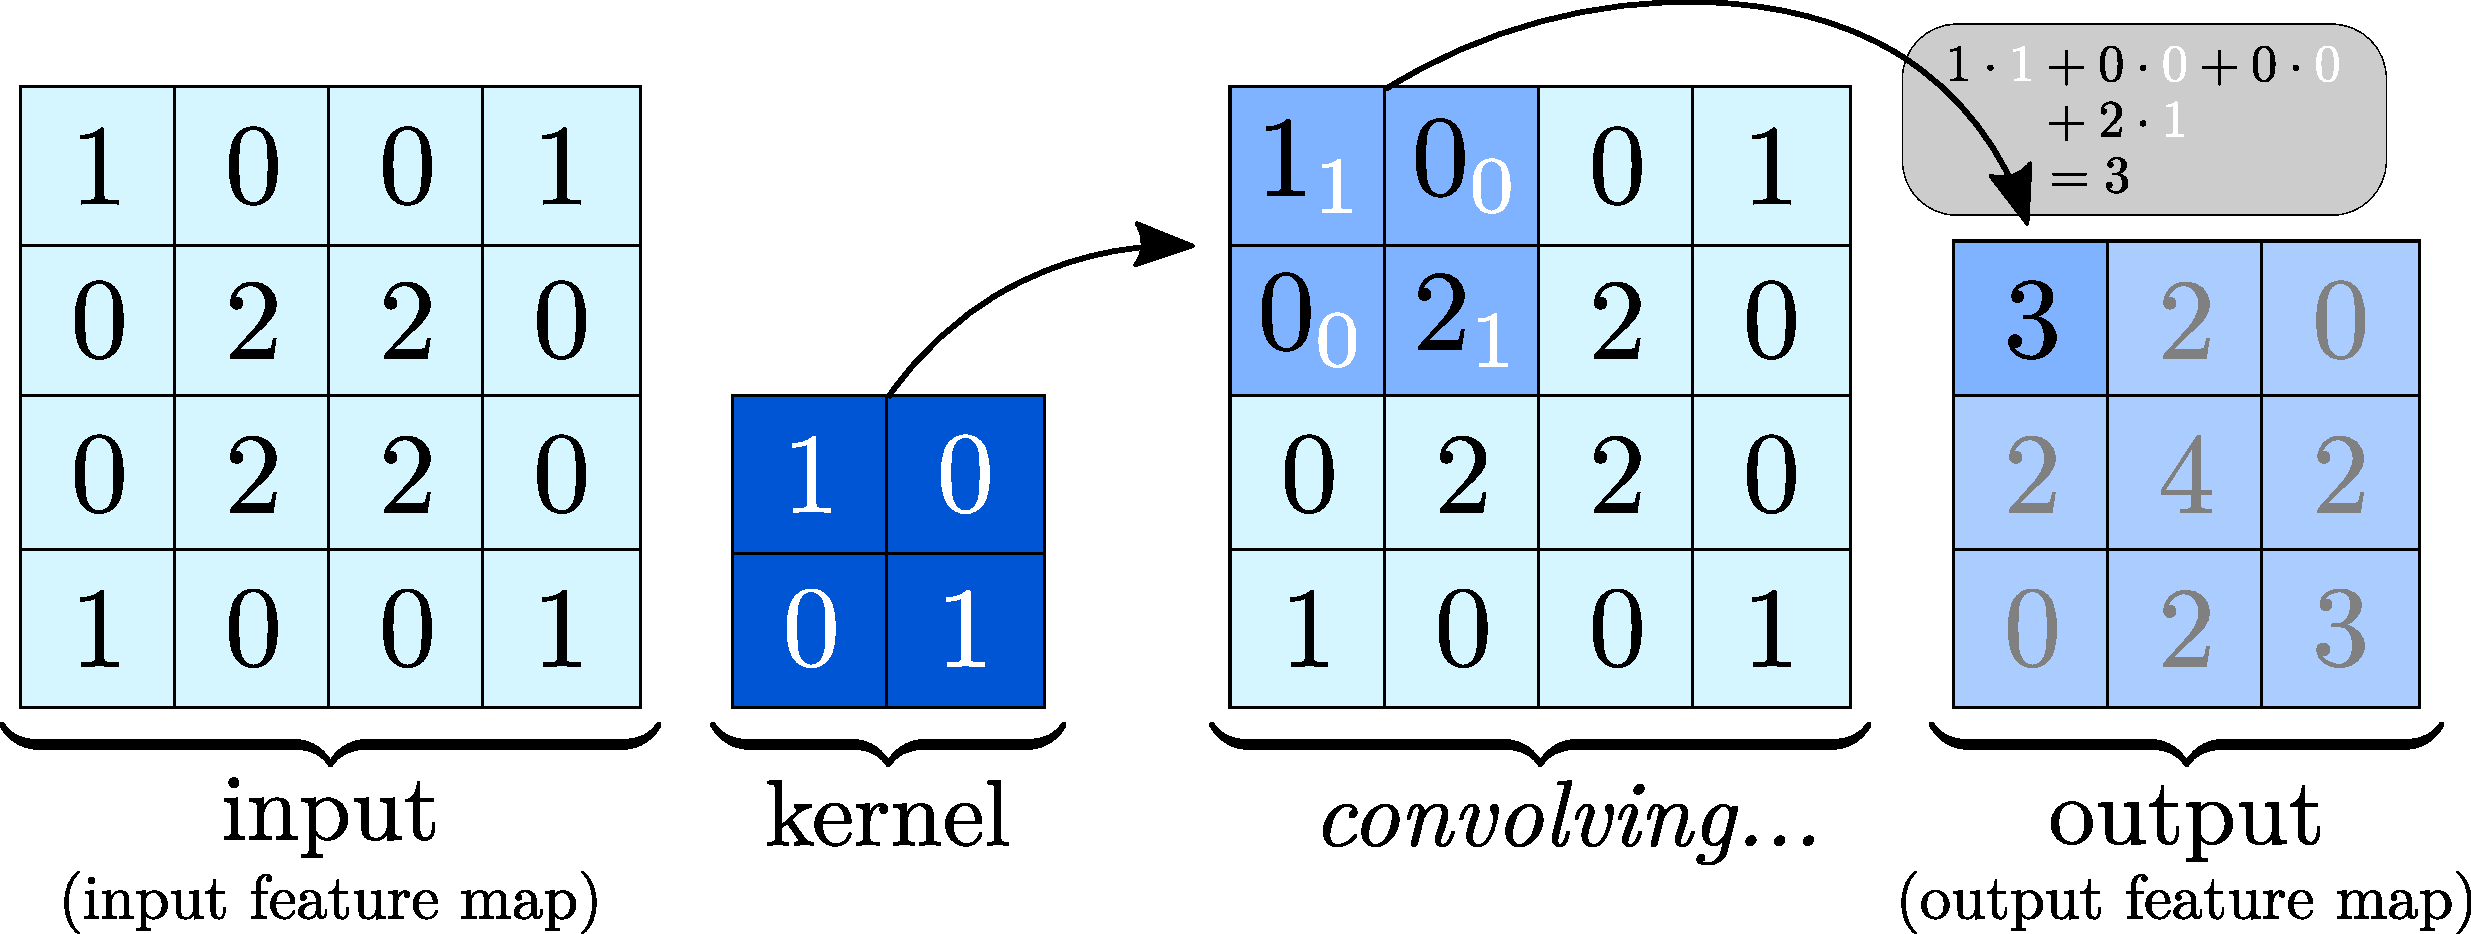
\includegraphics[width=\linewidth]{vector/conv-single-channel.pdf}
    \end{figure}

\end{frame}

\begin{frame}
    \frametitle{Discrete Convolution Examples}

    \only<1>{ \vspace{10mm}
    \makebox[\textwidth][c]{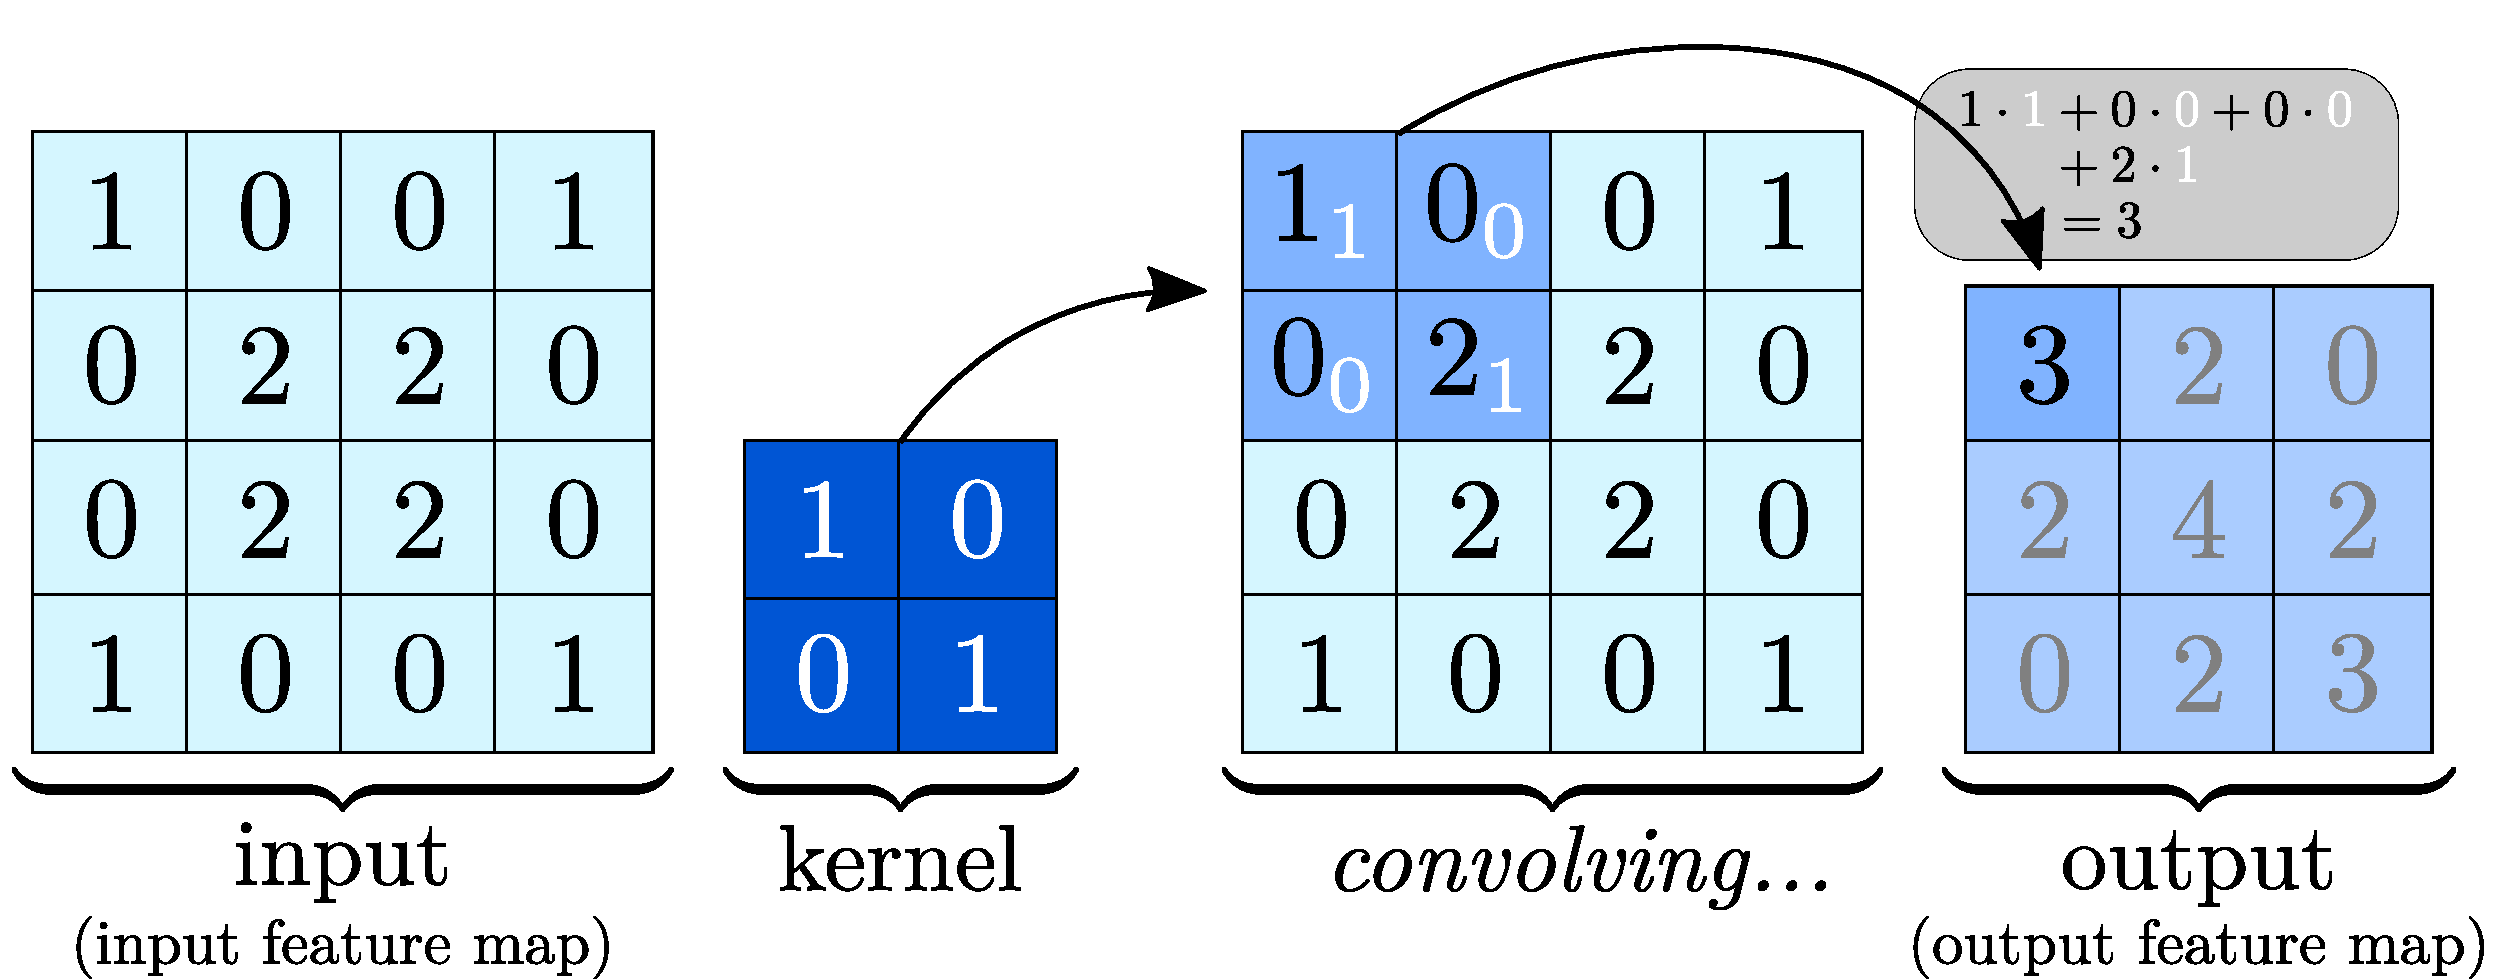
\includegraphics[width=0.99\paperwidth]{vector/figures-presentation/conv-single-channel-a.pdf}}}

    \only<2>{ \vspace{10mm}
    \makebox[\textwidth][c]{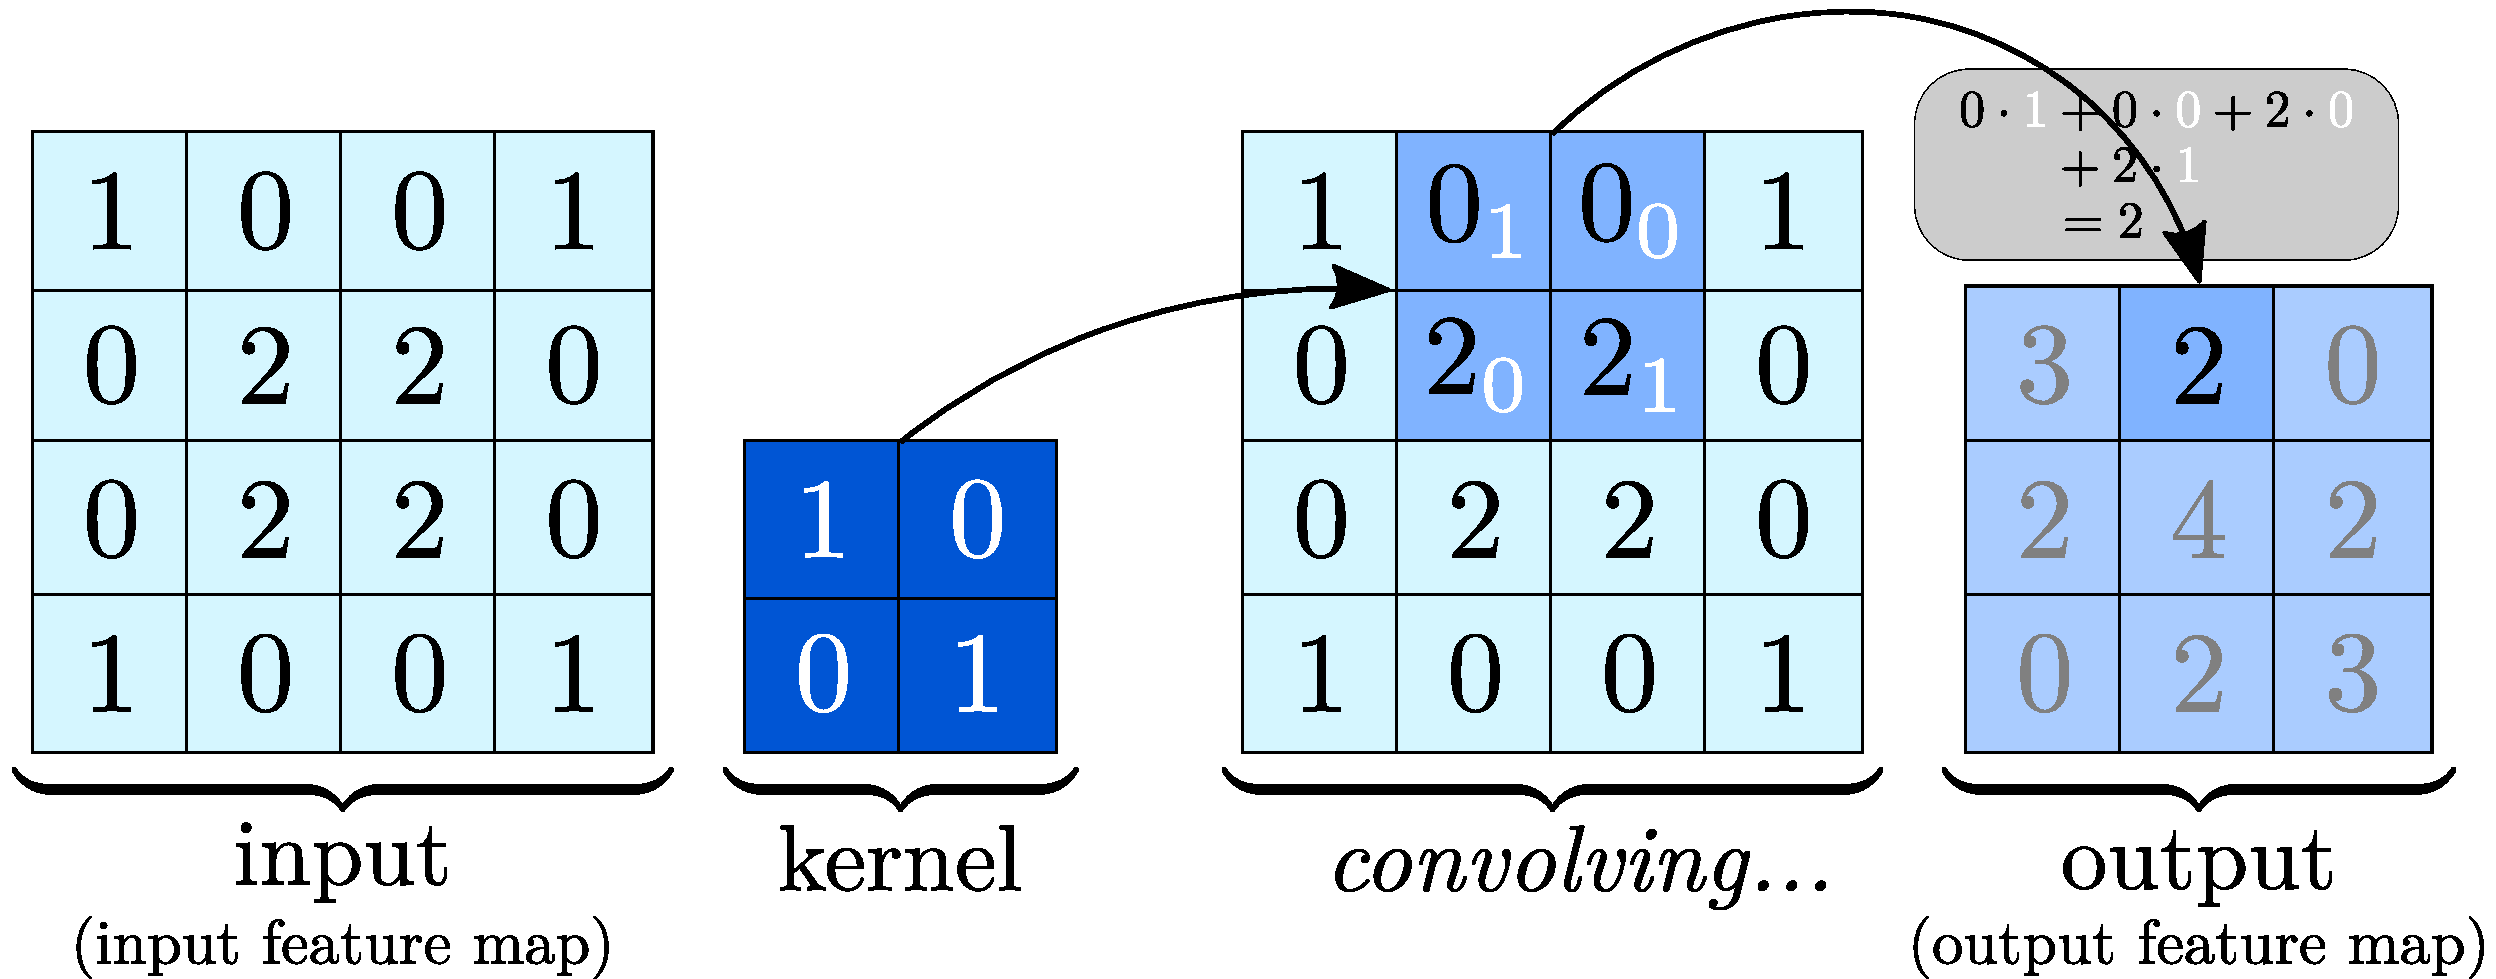
\includegraphics[width=0.99\paperwidth]{vector/figures-presentation/conv-single-channel-b.pdf}}}

    \only<3>{ \vspace{10mm}
    \makebox[\textwidth][c]{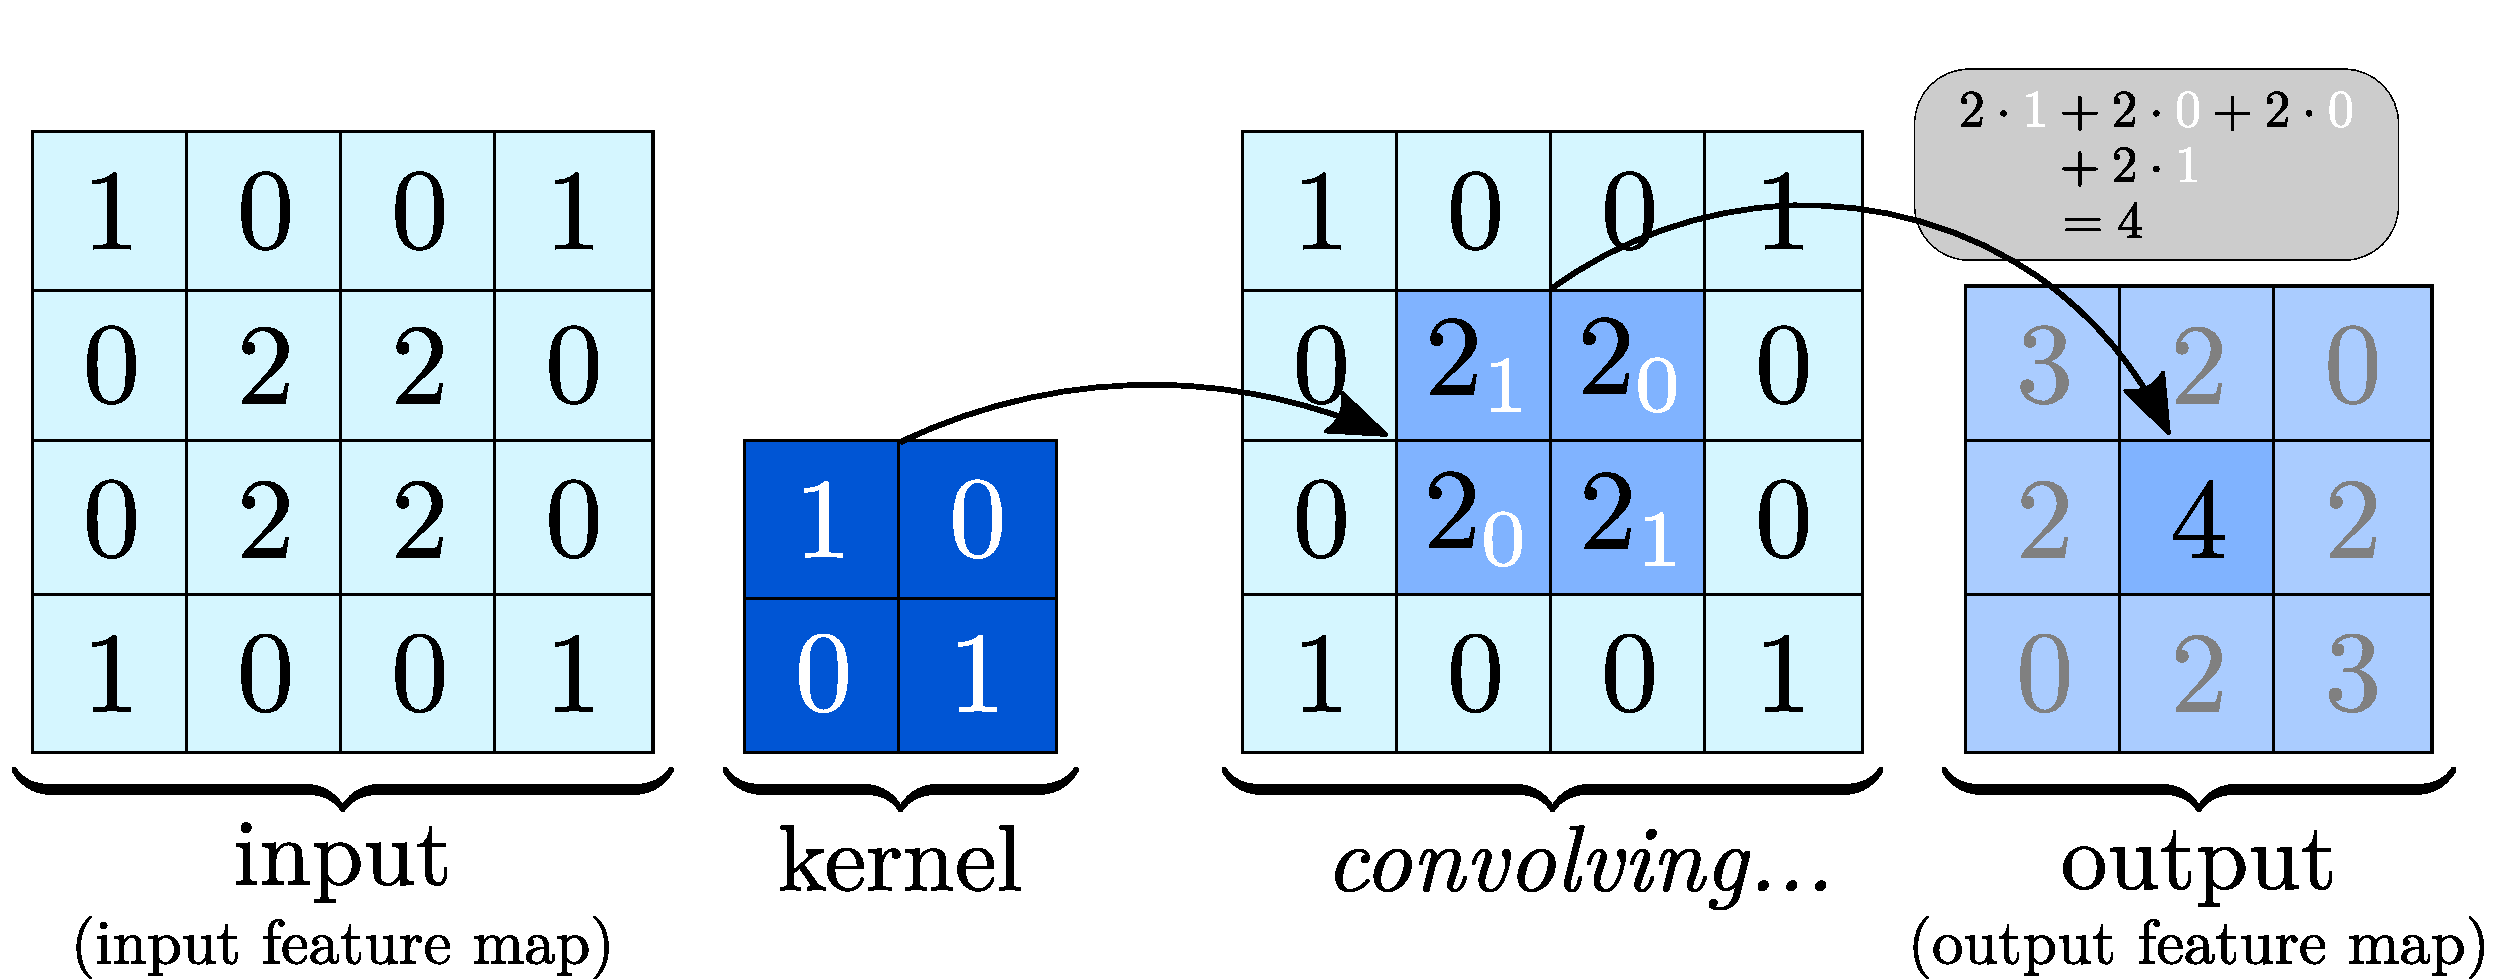
\includegraphics[width=0.99\paperwidth]{vector/figures-presentation/conv-single-channel-c.pdf}}}

    % numbers in input are pixel values, which represent deposited energy at a location in the detector

\end{frame}

\begin{frame}
    \frametitle{Generalizations...}

    \underline{Multi-channel images}
    \begin{itemize}
    
        \item Input images (3D) have multiple channels...

        \item So use a multi-channel (3D) kernel!

        \item Sum across channel axis to get 2D output
    
    \end{itemize}

    \begin{figure}[htb!]
    \centering
    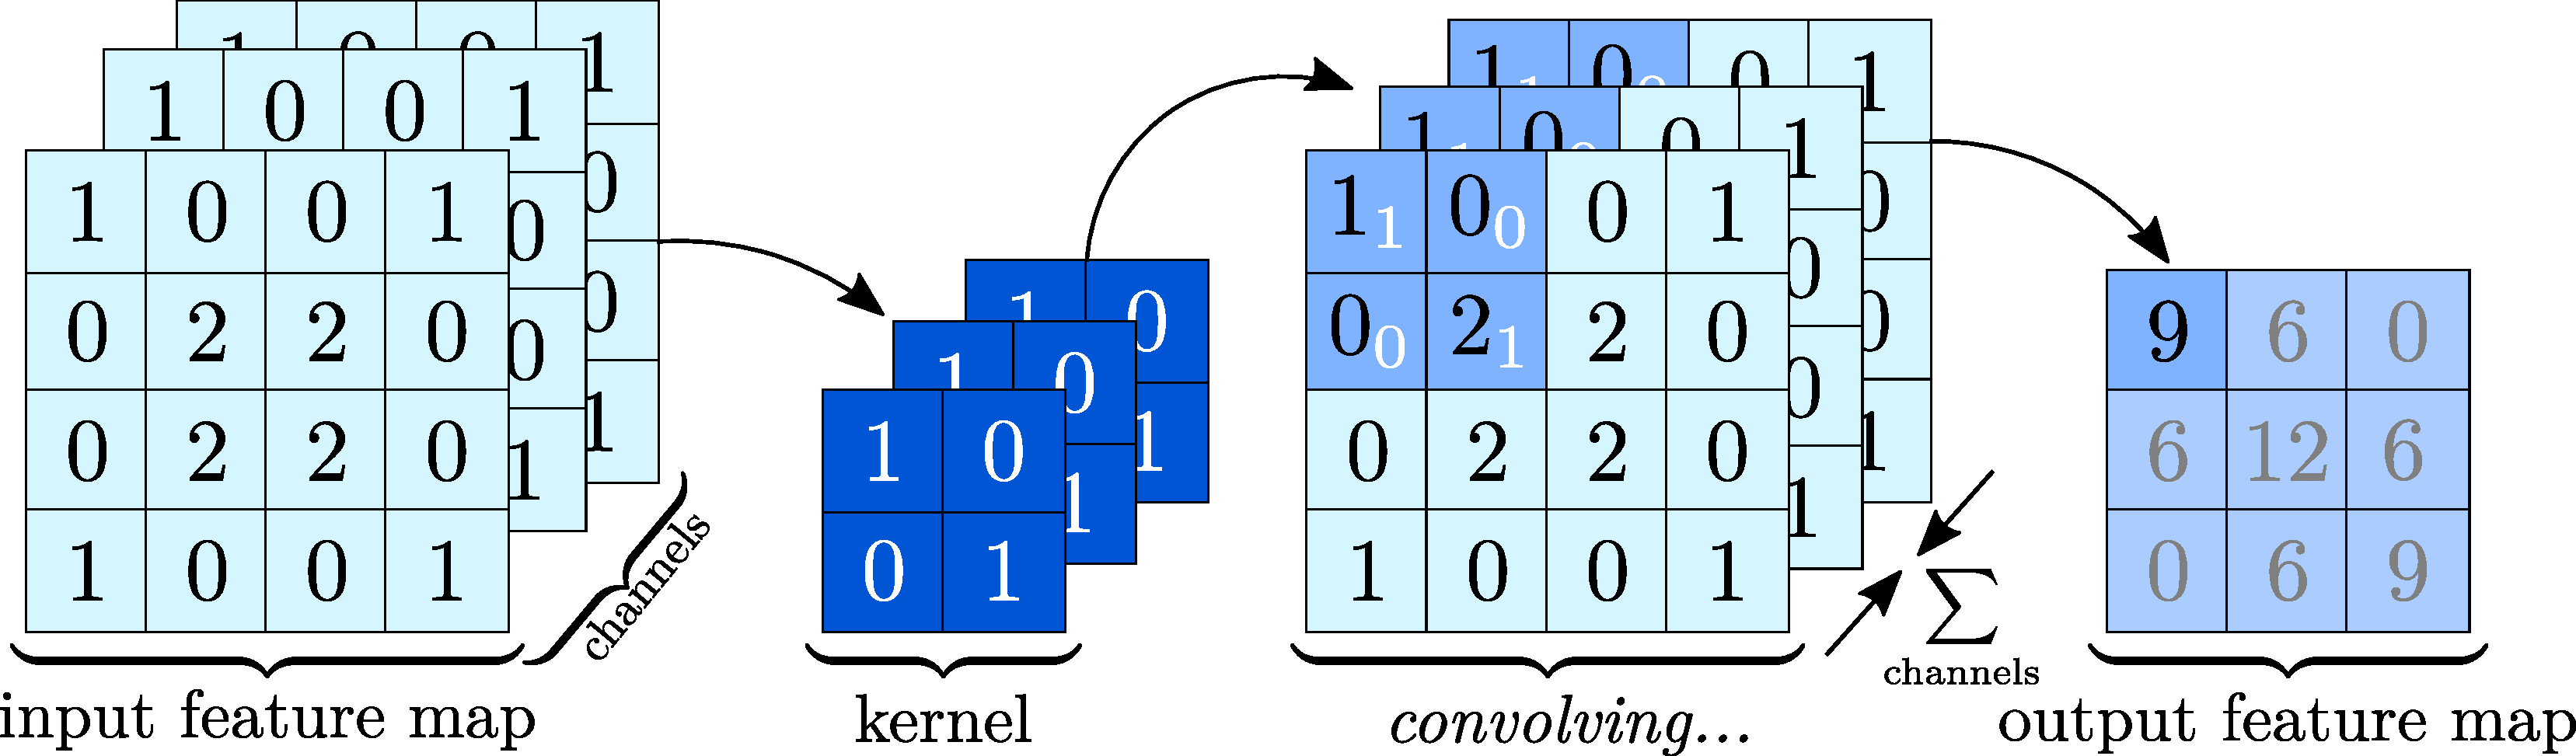
\includegraphics[width=\linewidth]{vector/conv-multi-channel.pdf}
    \end{figure}

\end{frame}

\begin{frame}
    \frametitle{Generalizations...}

    \underline{Multiple kernels}
    \begin{itemize}
    
        \item Like multiple neurons in an FCN

        \item Each kernel captures a specific feature\\
        {\small (edges, curves contrasting colors, shapes...)}

        \item Output feature map is then 3D
    
    \end{itemize}

    \begin{figure}[htb!]
    \centering
    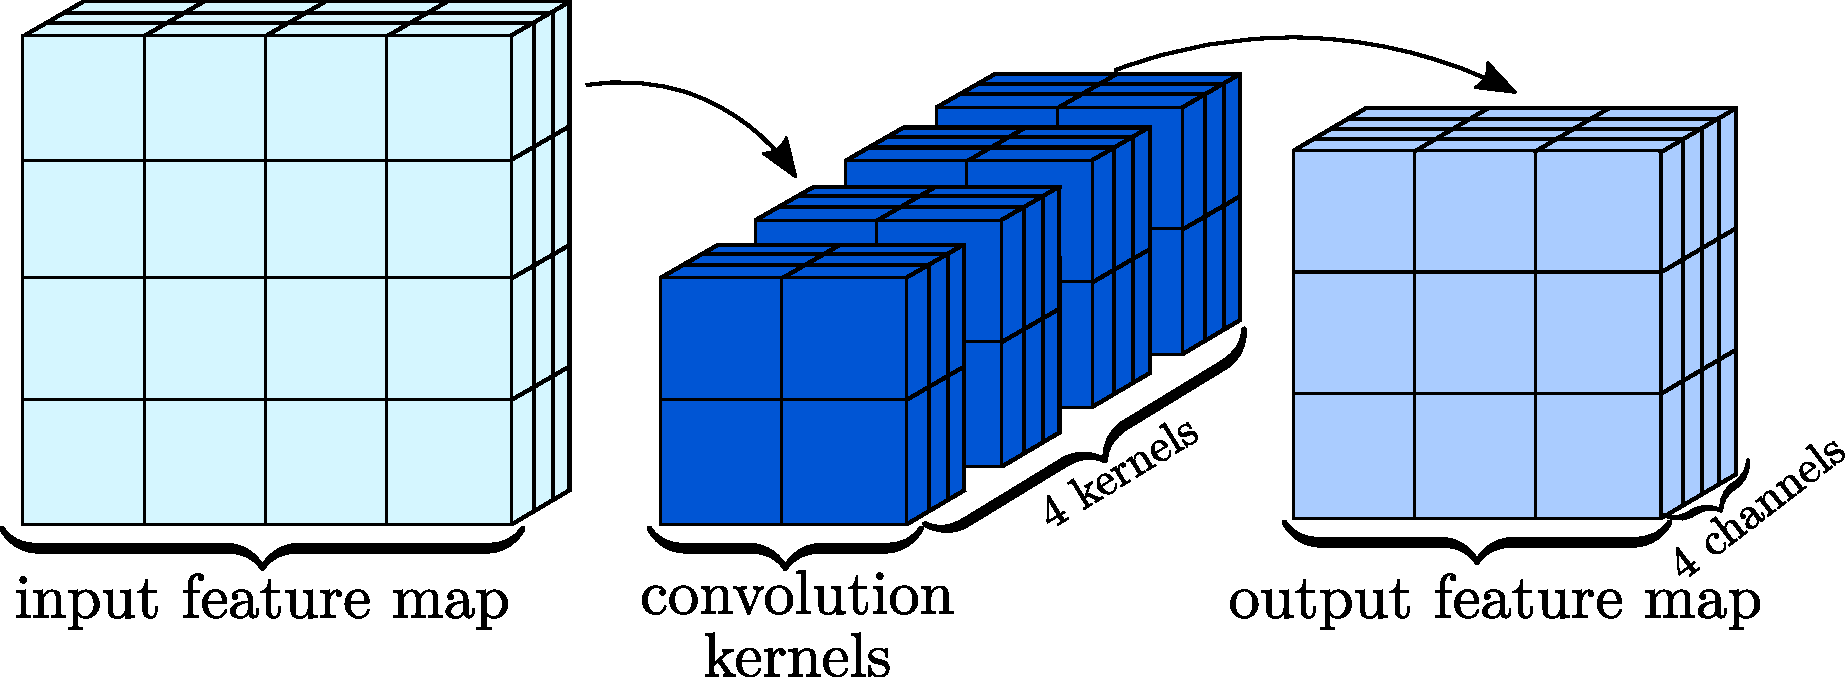
\includegraphics[width=\linewidth]{vector/figures-presentation/cnn-multi-kernel.pdf}
    \end{figure}   

\end{frame}

\begin{frame}
    \frametitle{(Max) Pooling}

    Goals:
    \begin{itemize}
    
        \item spatially downsample input
    
        \item introduce invariance to local translations

        \item preserve channel dimension

    \end{itemize}
    \vspace{1mm}
    \onslide<2->{Operation: A \textit{pooling kernel} outputs maximum pixel value at each kernel position in input}
    \vspace{-1mm}
    \begin{figure}[htb!]
        \centering
        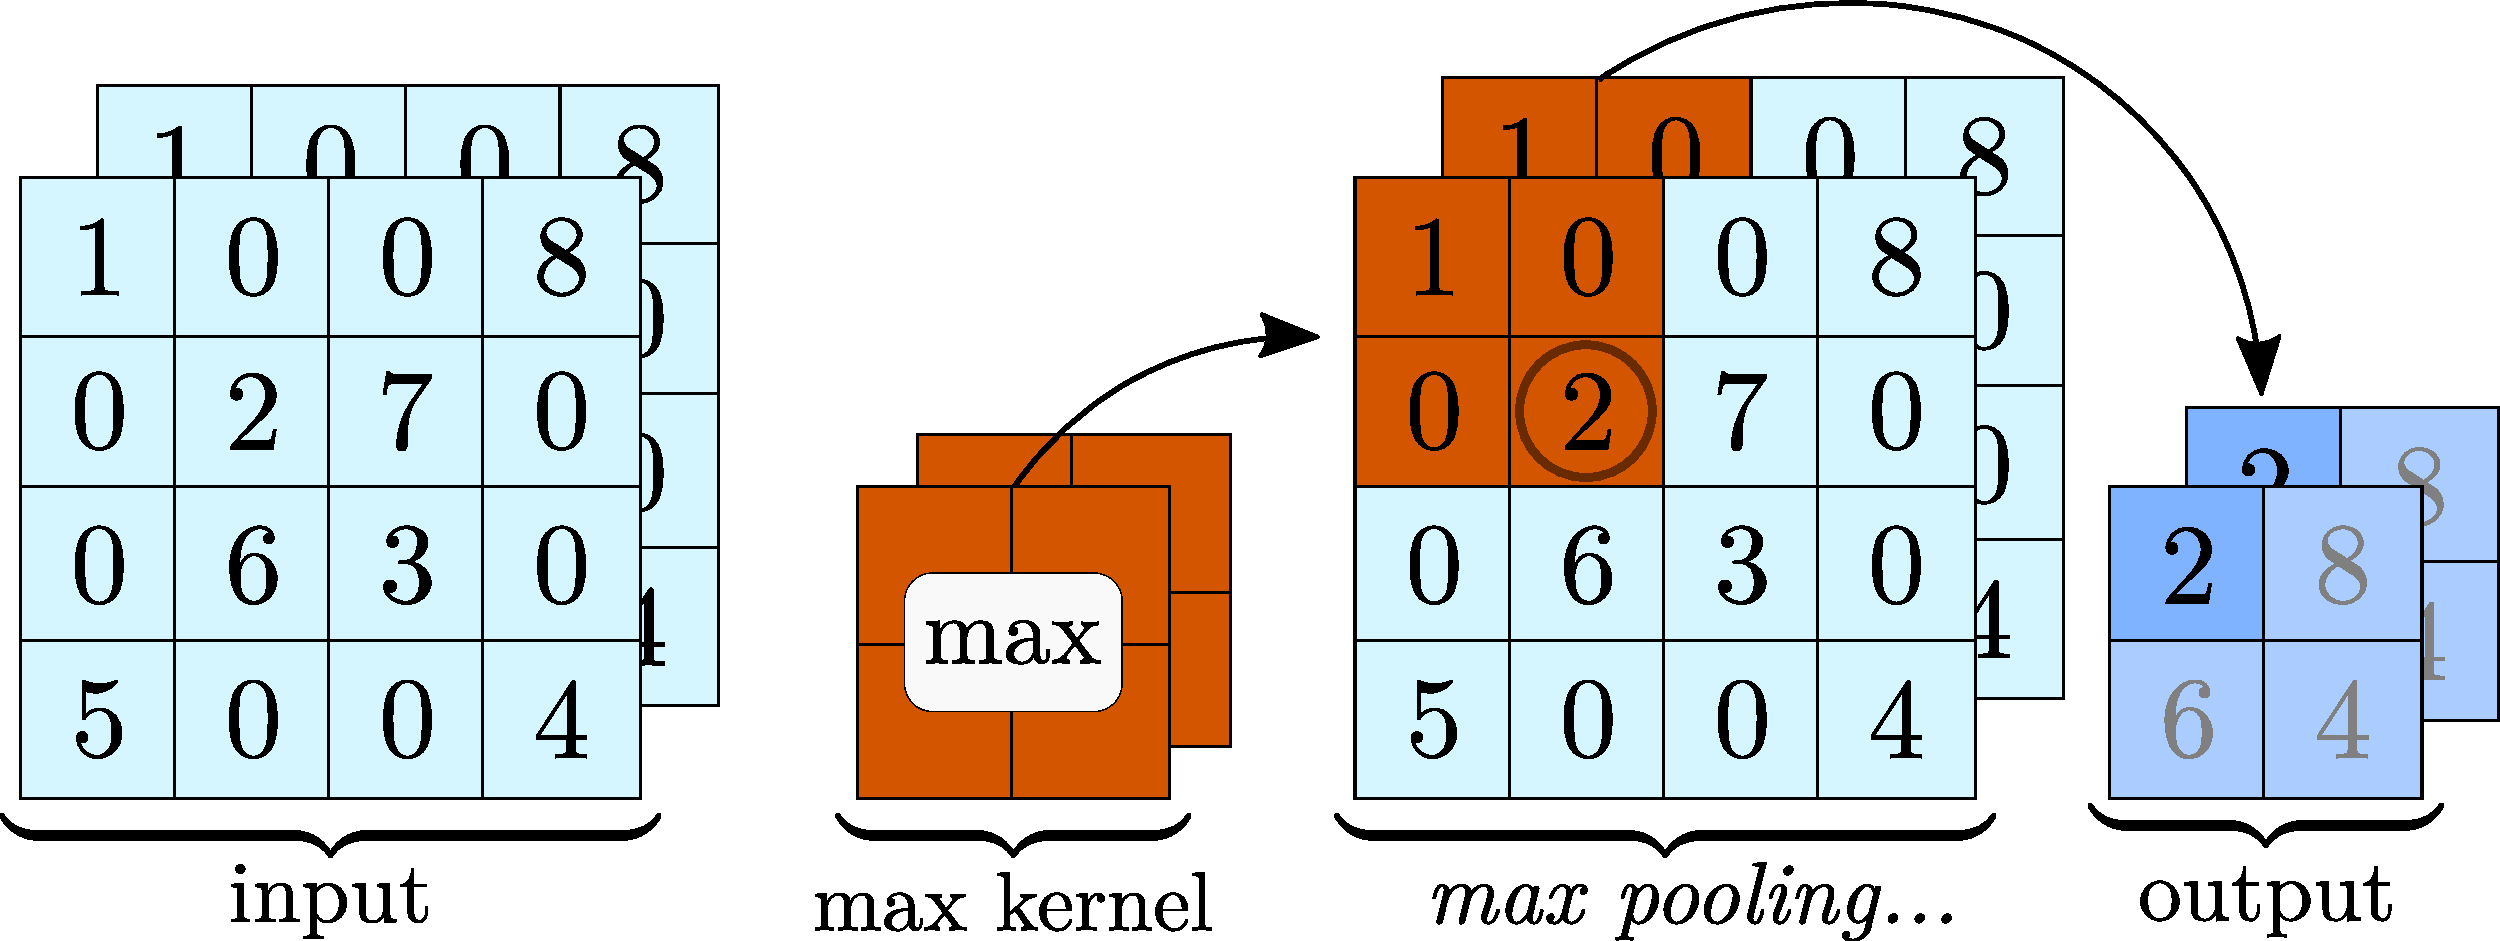
\includegraphics[width=\linewidth]{vector/pooling.pdf}
    \end{figure}   

\end{frame}

\begin{frame}
    \frametitle{Max Pooling Examples}

    \only<1>{ \vspace{10mm}
    \makebox[\textwidth][c]{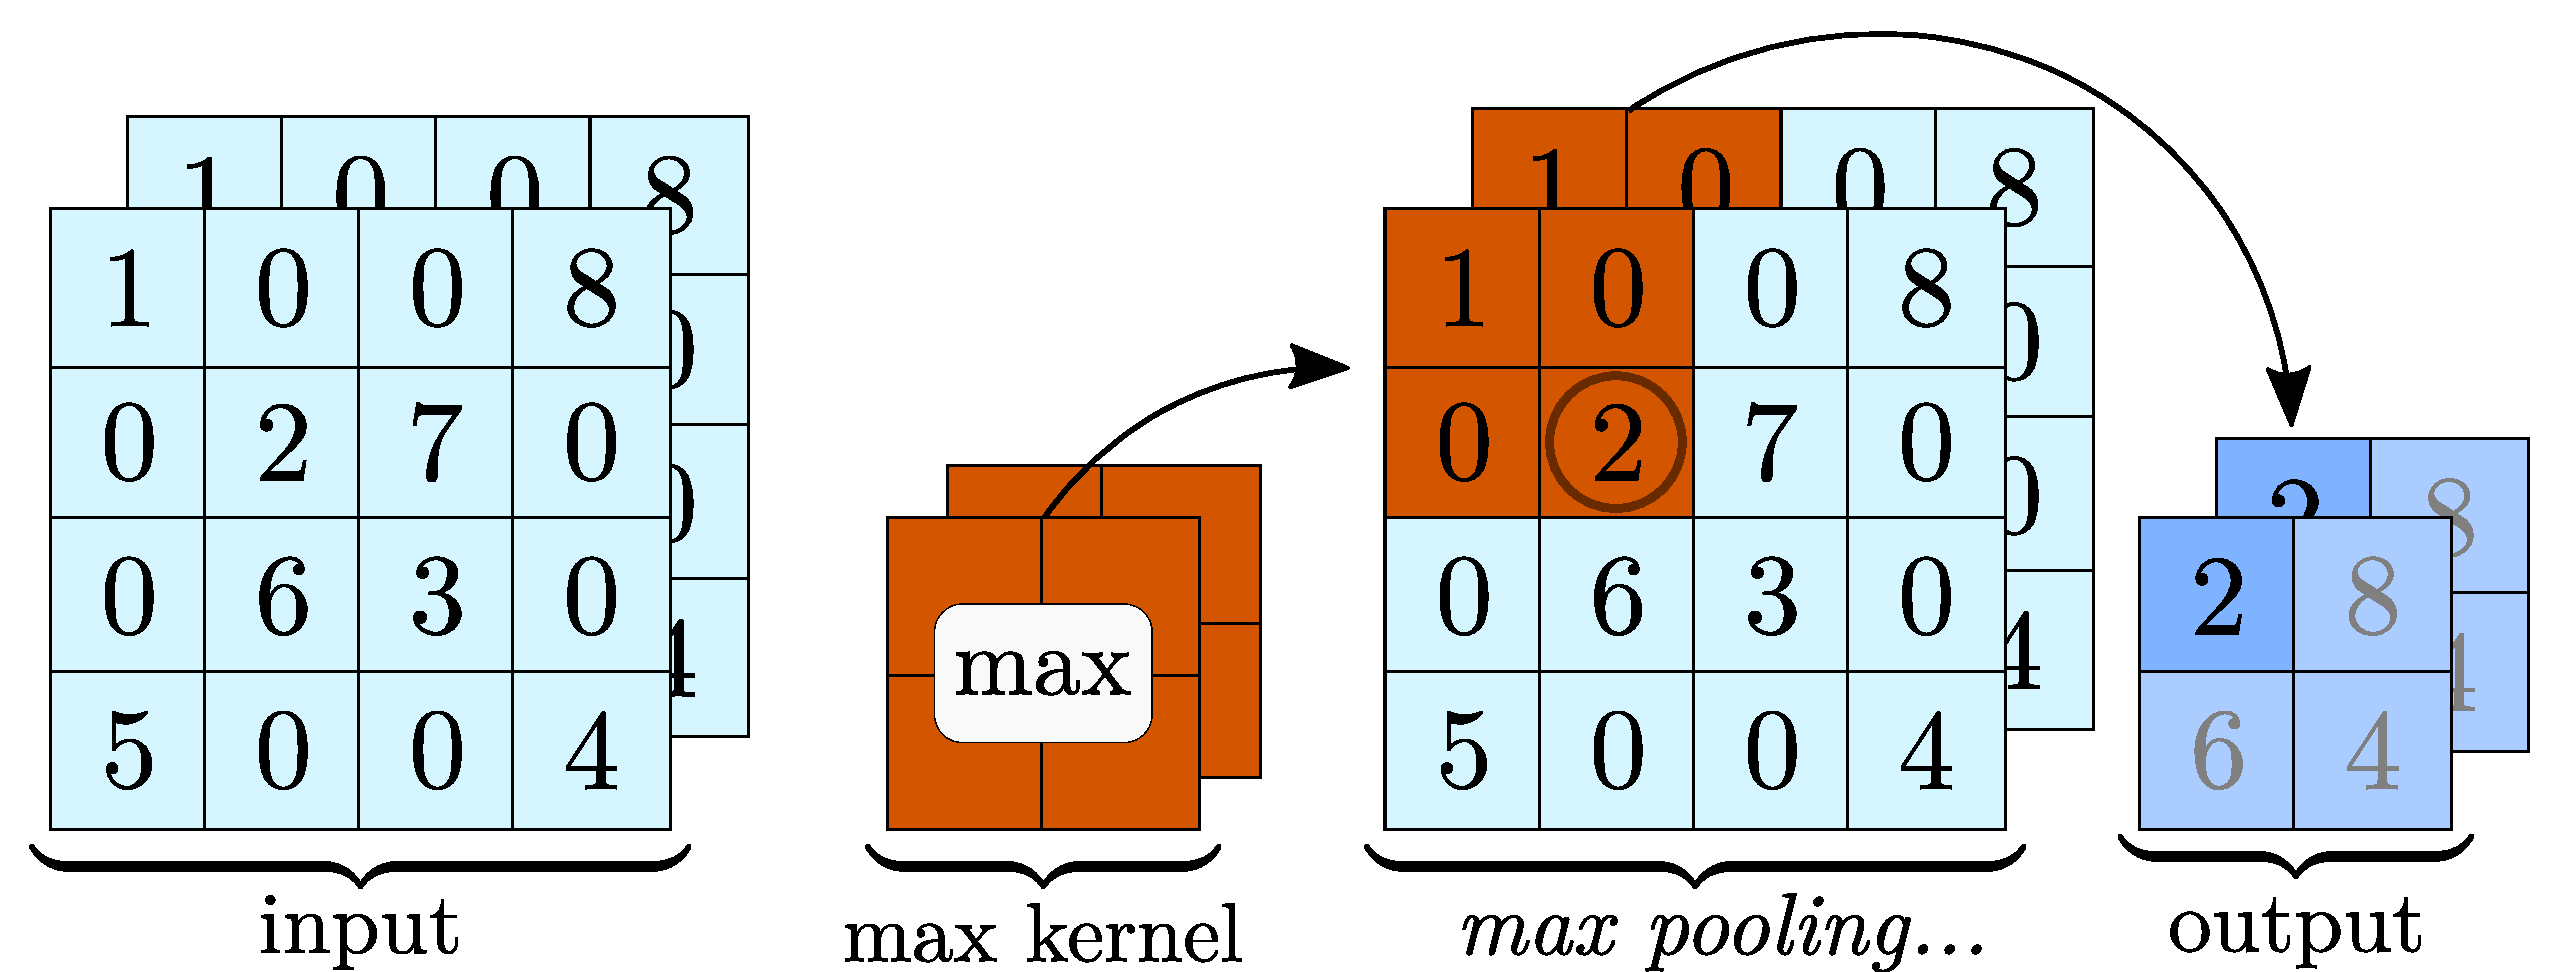
\includegraphics[width=0.99\paperwidth]{vector/figures-presentation/pooling-a.pdf}}}

    \only<2>{ \vspace{10mm}
    \makebox[\textwidth][c]{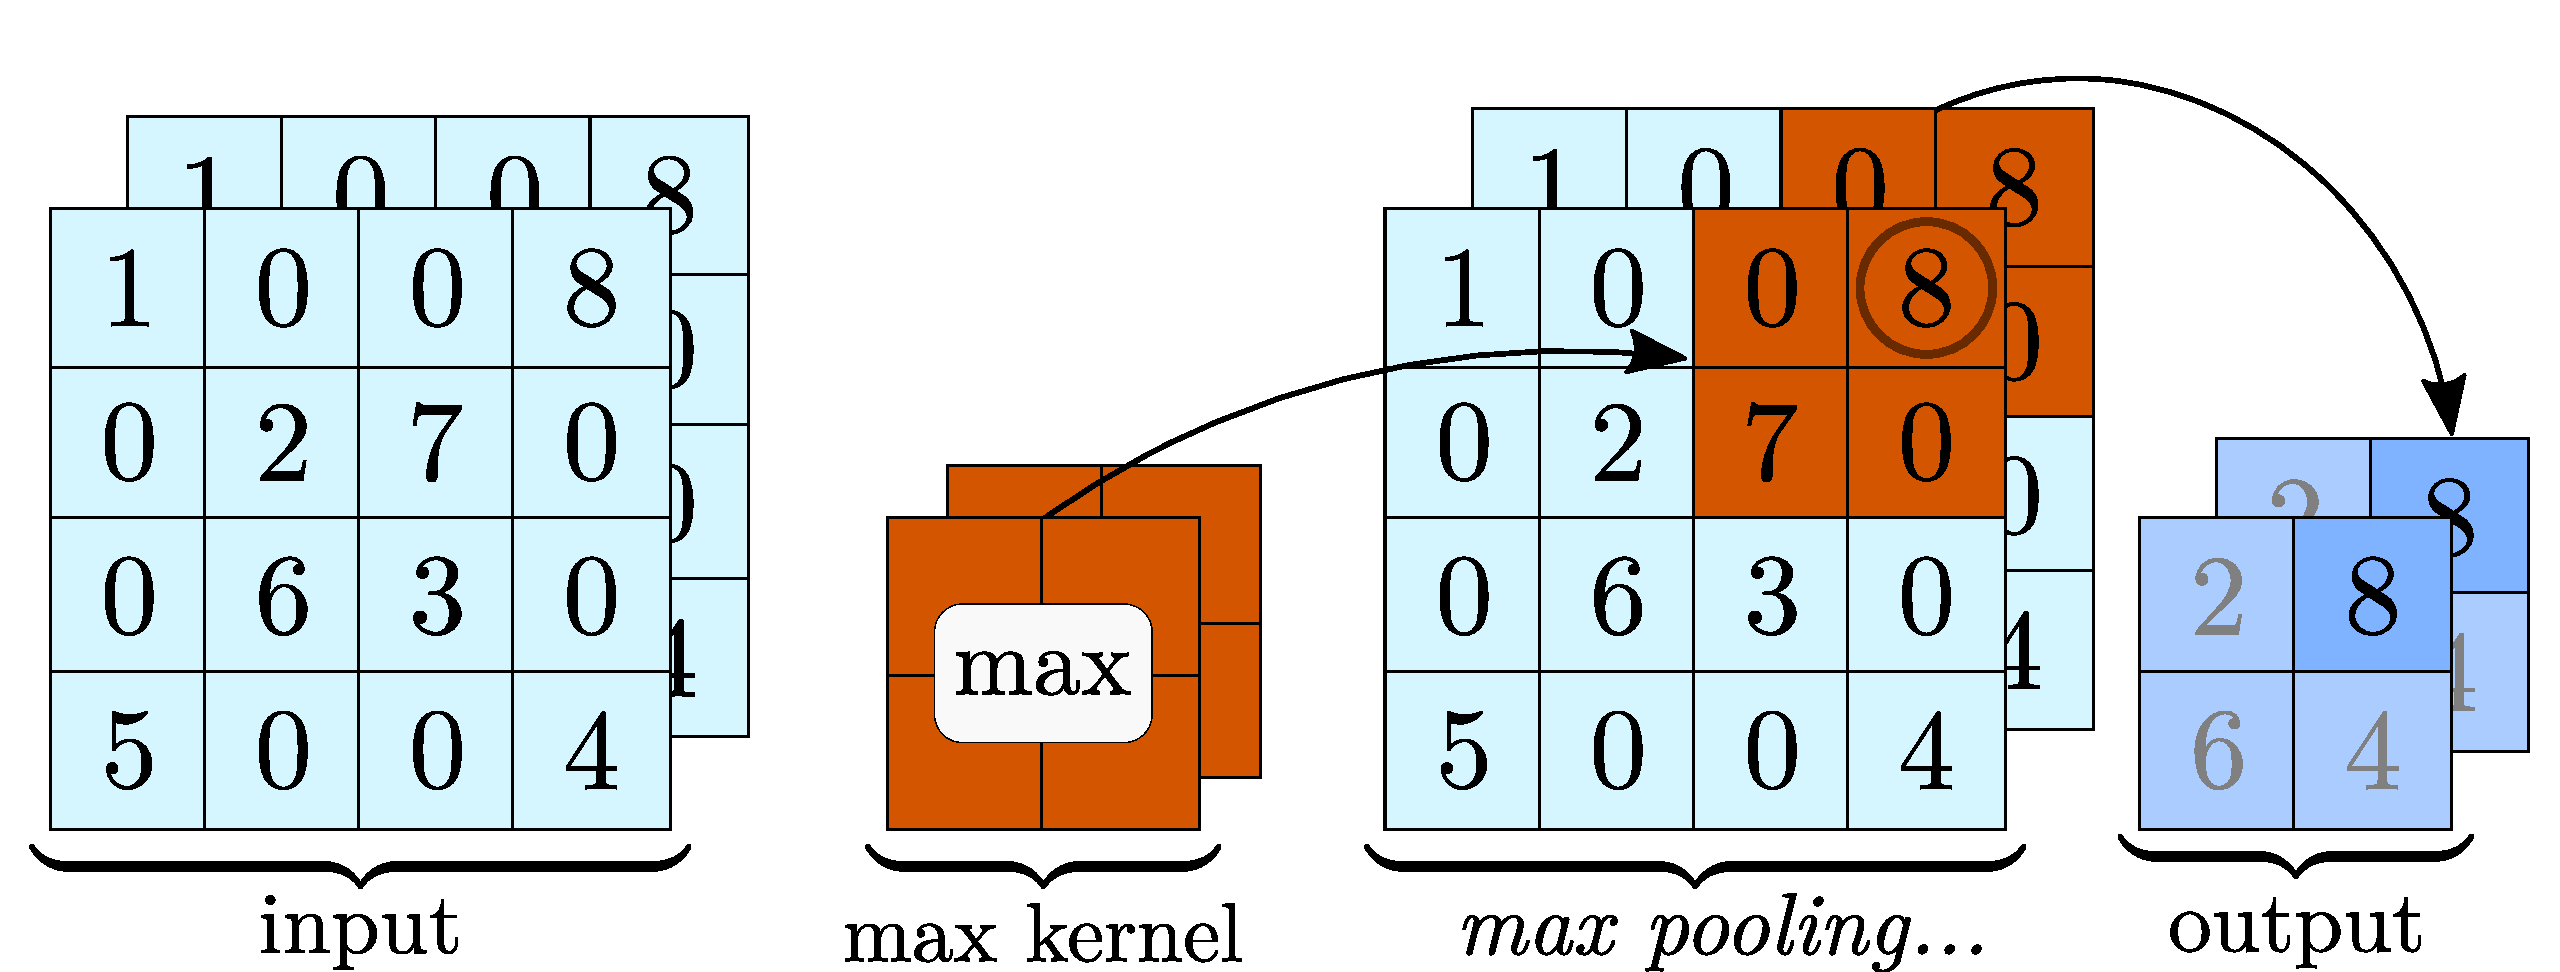
\includegraphics[width=0.99\paperwidth]{vector/figures-presentation/pooling-b.pdf}}}

    \only<3>{ \vspace{10mm}
    \makebox[\textwidth][c]{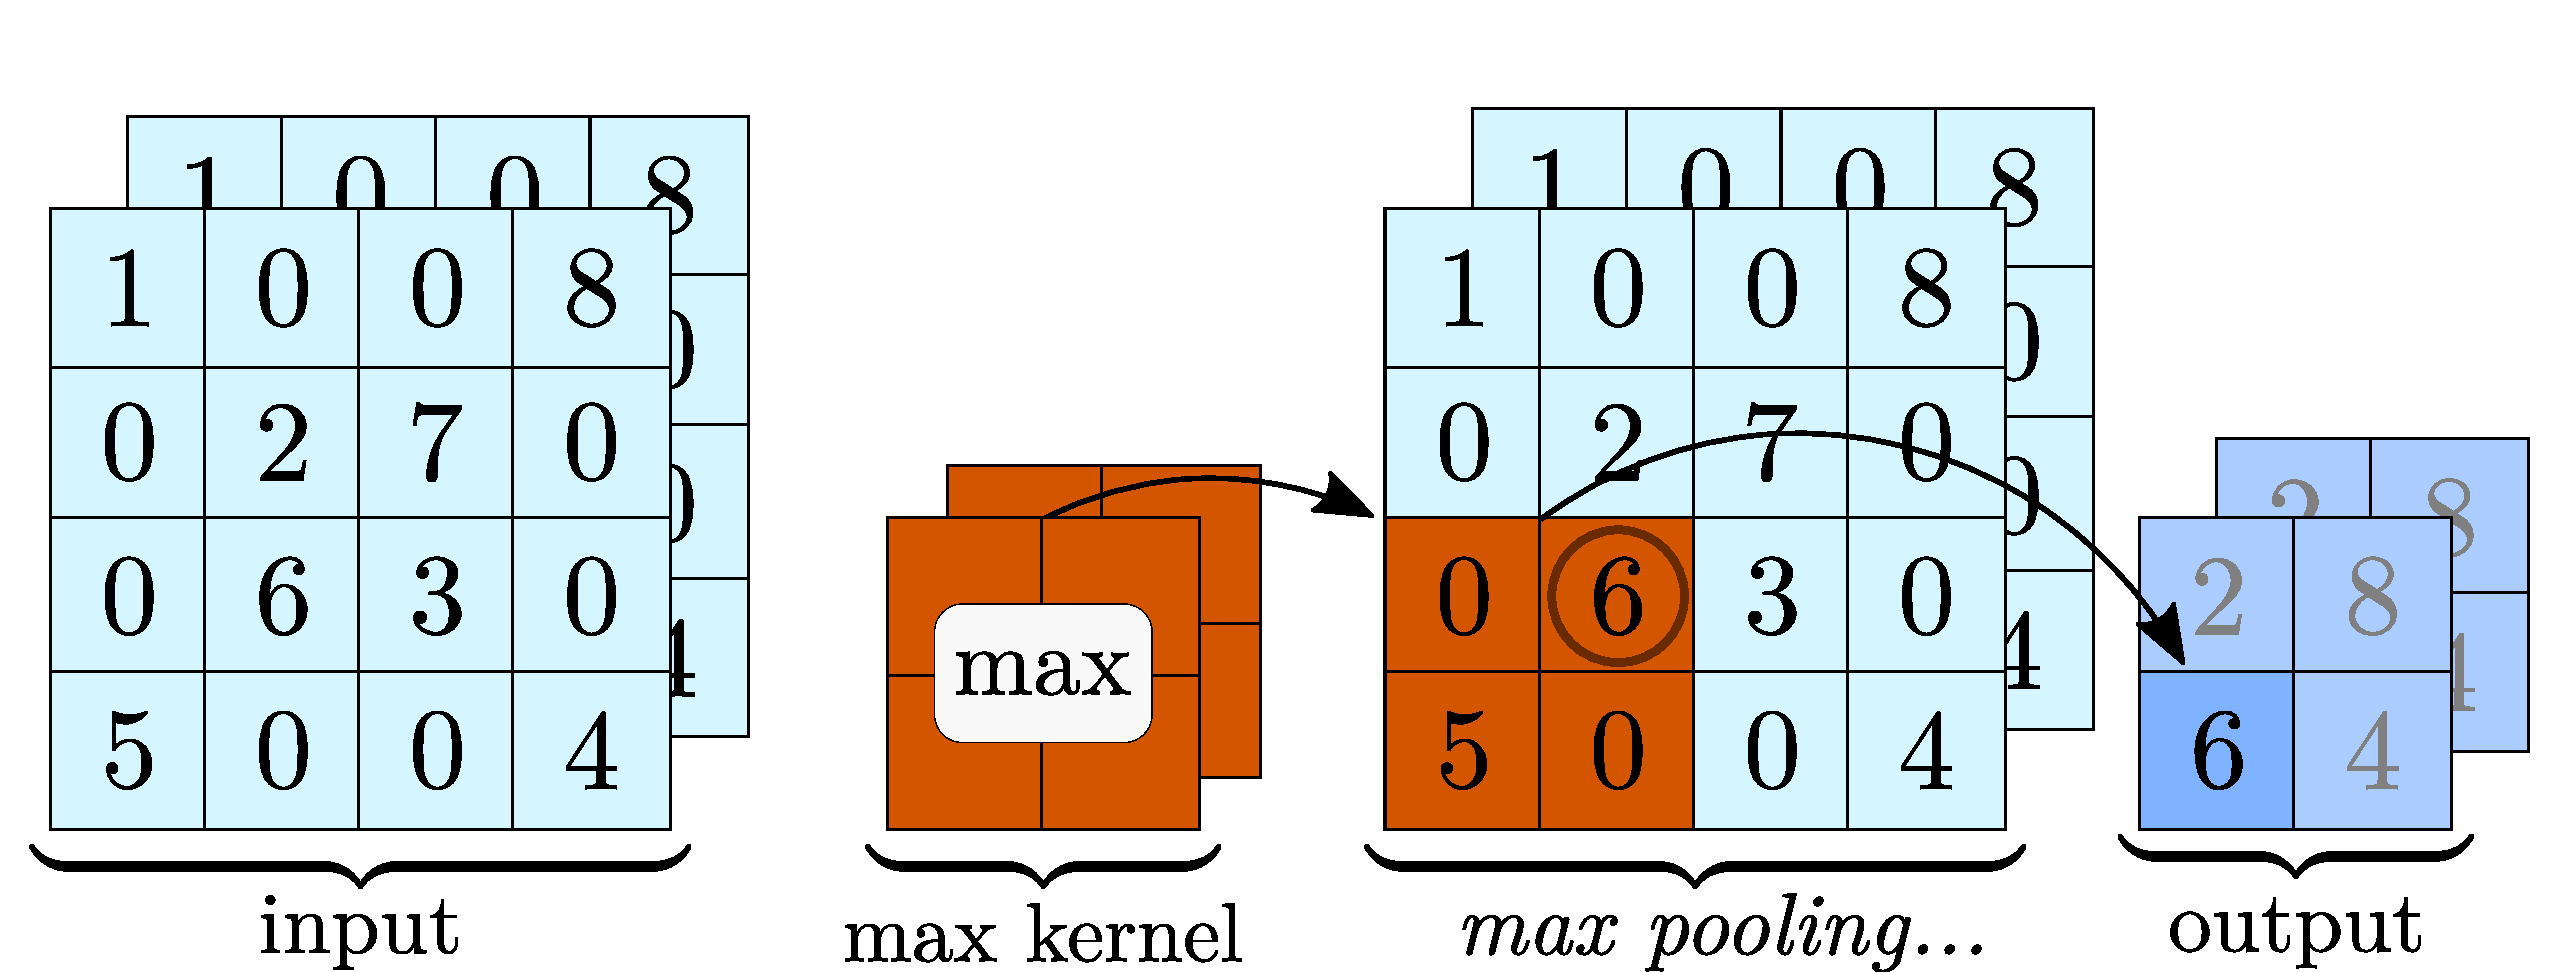
\includegraphics[width=0.99\paperwidth]{vector/figures-presentation/pooling-c.pdf}}}

    \only<4>{ \vspace{10mm}
    \makebox[\textwidth][c]{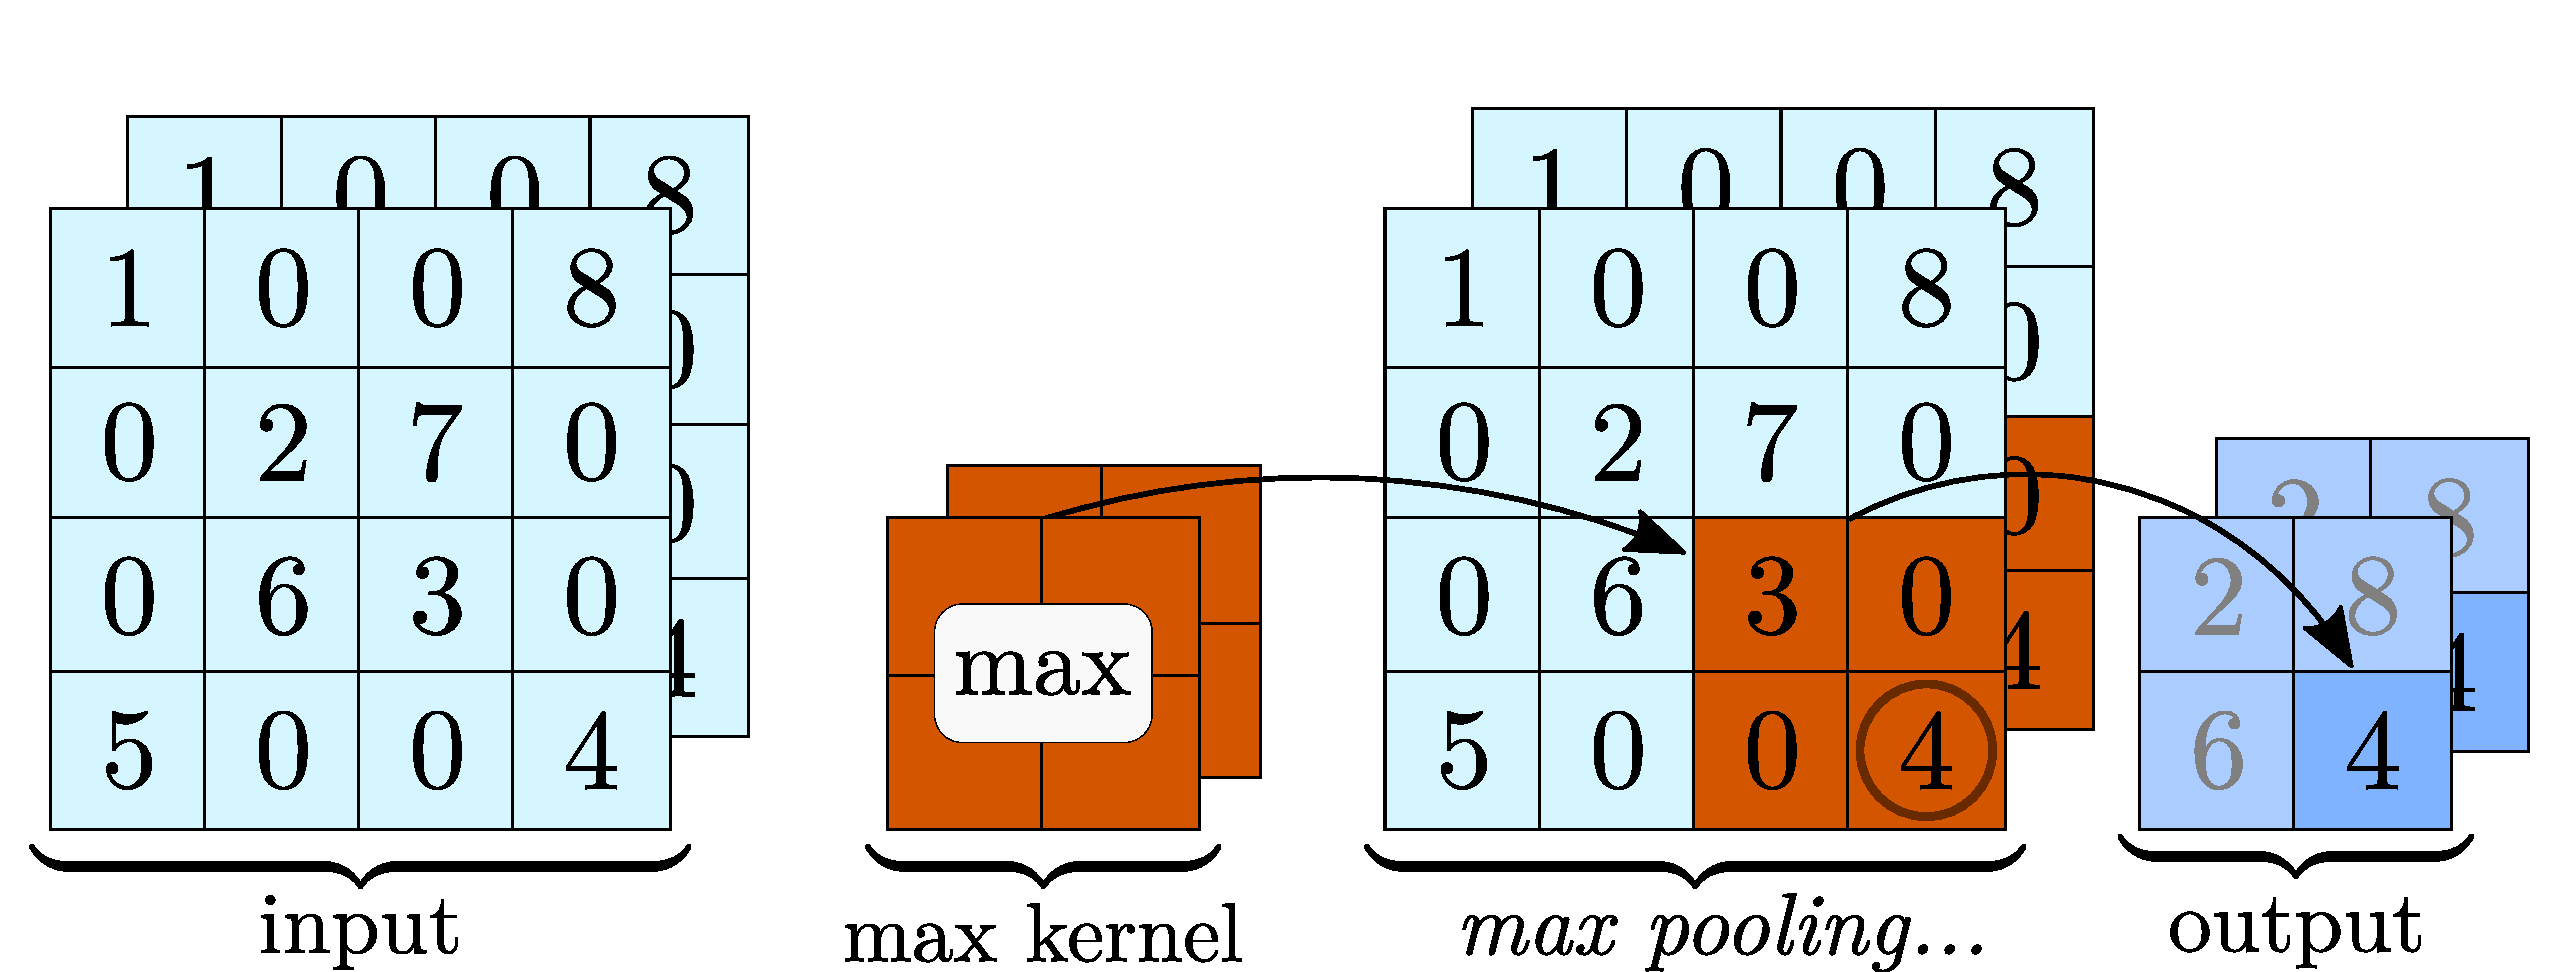
\includegraphics[width=0.99\paperwidth]{vector/figures-presentation/pooling-d.pdf}}}

\end{frame}

\begin{frame}
    \frametitle{CNN Architecture}
    
    \onslide<1-3>{
    Typical convolutional layer sequence:
    \begin{enumerate}[(a)]
    
        \item convolution

        \item non-linearity (e.g. ReLU)

        \item pooling
    
    \end{enumerate}}
    \onslide<2-3>{Repeat... (not shown)\\}
    \onslide<3>{Flatten; use fully-connected layer for output}

    \only<1-2>{
    \begin{figure}[htb!]
        \centering
        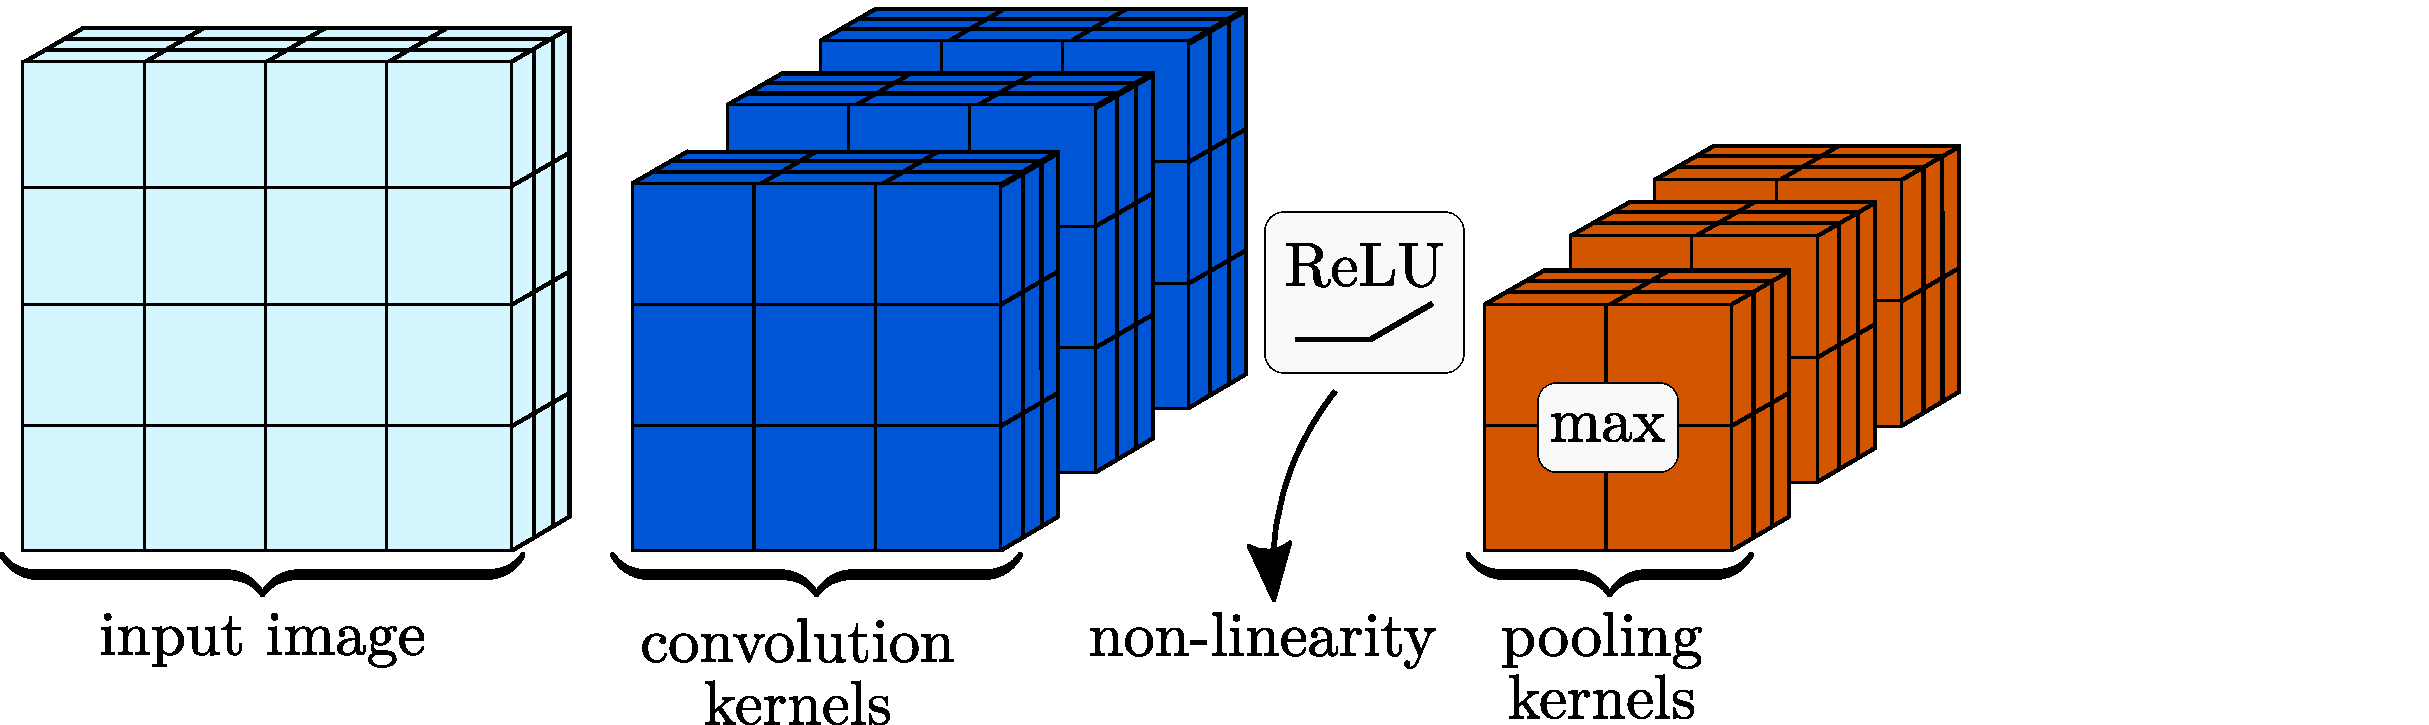
\includegraphics[width=\linewidth]{vector/figures-presentation/cnn-layer-sequence-a.pdf}
    \end{figure}}

    \only<3>{
    \begin{figure}[htb!]
        \centering
        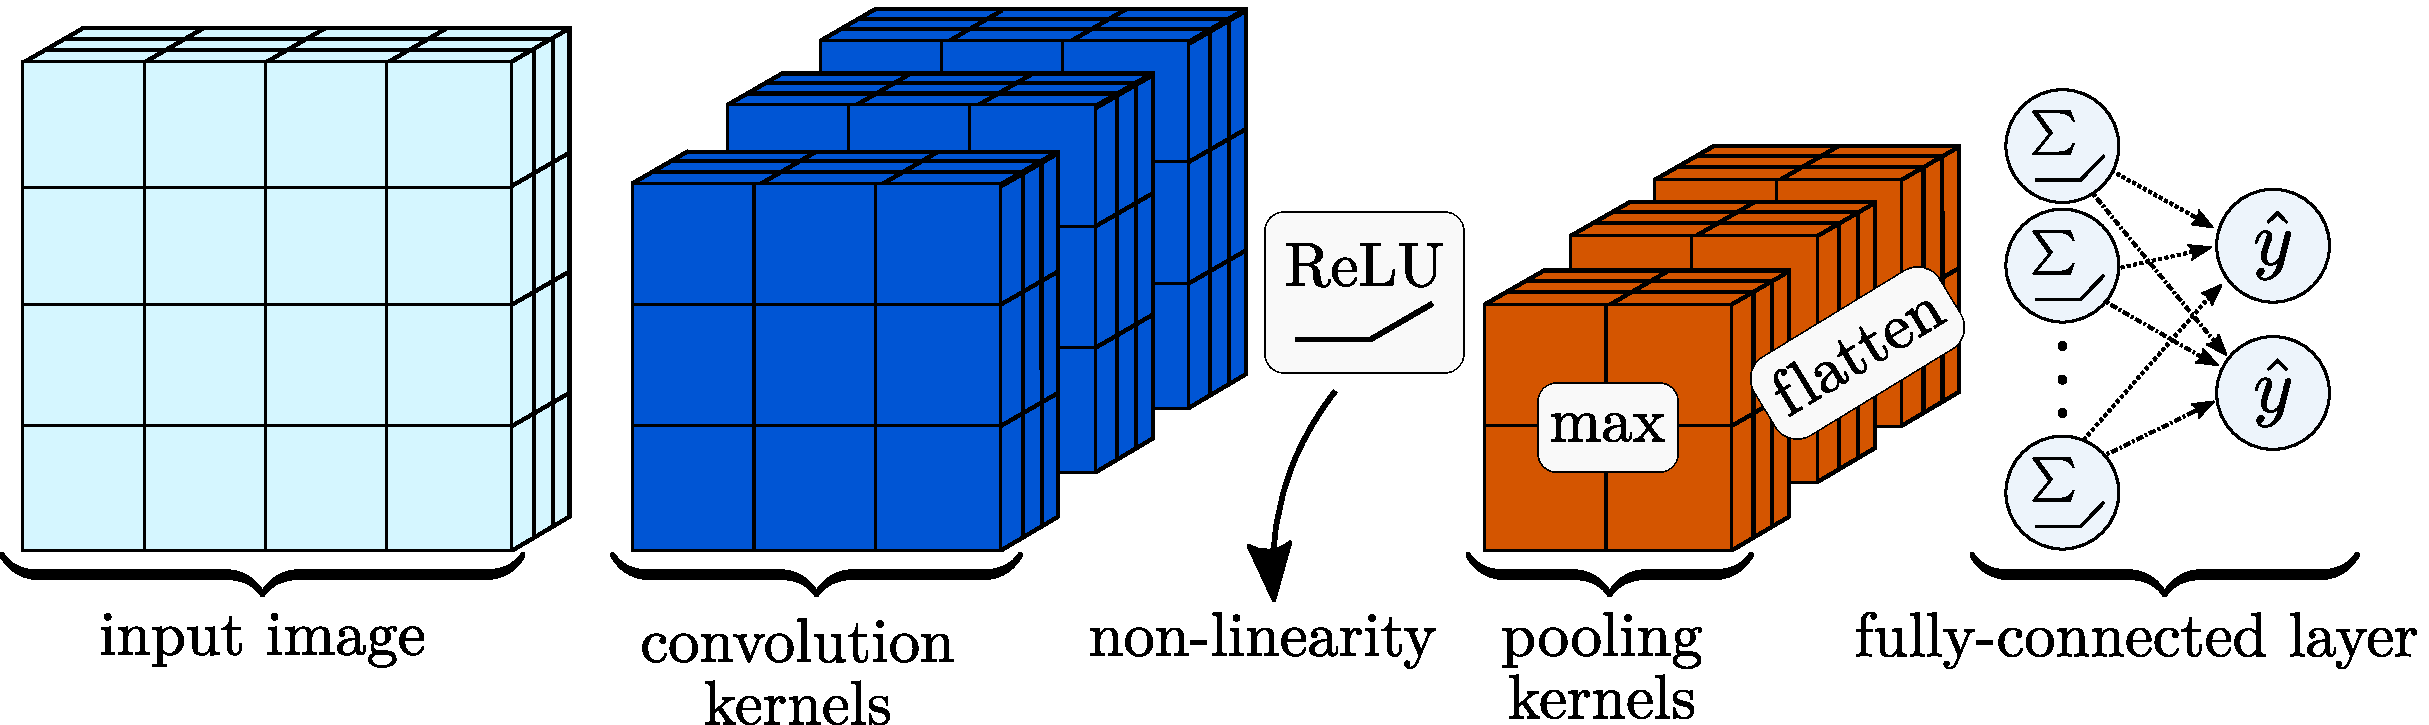
\includegraphics[width=\linewidth]{vector/figures-presentation/cnn-layer-sequence-b.pdf}
    \end{figure}}

\end{frame}

\section{End-to-End Classification in Practice}
\begin{frame}
    \frametitle{A Concrete Case Study}

    Andrews et al. \textit{End-to-End Physics Event Classification with CMS Open Data}. 2020. \cite{andrews-higgs}

    \begin{itemize}
    
        \item Higgs boson classification with CMS data

        \item Signal: $ gg \to H^{0} \to \gamma \gamma $

        \item Background 1: $ q \bar{q} \to \gamma \gamma $

        \item Background 2: $ q \bar{q} \to \gamma j $
    
    \end{itemize}

    \begin{figure}[htb!]
        \centering
        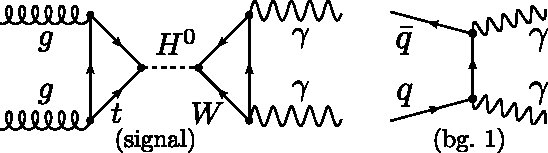
\includegraphics[width=\linewidth]{vector/figures-presentation/feynman.pdf}
    \end{figure}
    
\end{frame}

\begin{frame}
    \frametitle{Why the Processes Are Interesting}

    \begin{enumerate}[(a)]
    
        \definecolor{irrBgRed}{RGB}{175,0,0}
        \item<1-> {\color{irrBgRed} irreducible backgrounds}
        \begin{figure}[htb!]
            \centering
            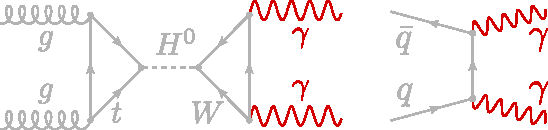
\includegraphics[width=\linewidth]{vector/figures-presentation/feynman-irr-bg.pdf}
        \end{figure}

        \item<2-> unresolved decay products
        \vspace{-3mm}
        \begin{equation*}
            \gamma j \approx \gamma \gamma \implies \text{bg 1} \approx \text{bg 2} \approx \text{sig}
        \end{equation*}
    \end{enumerate}

    \vspace{7mm}

    \makebox[\textwidth]{\parbox{1.185\textwidth}{%
        
    \rule{\paperwidth}{0.3pt}\\[-5mm]
    \vspace{-5mm}
    \begin{center}
        \small{for reference...}
        \vspace{-3mm}
        \begin{equation*}
            \text{sig:} \ gg \to H^{0} \to \gamma \gamma \qquad \text{bg 1:} \ q \bar{q} \to \gamma \gamma \qquad \text{bg 2:} \ q \bar{q} \to \gamma j
        \end{equation*}   
    \end{center}
    }}
    \vspace{-2mm}
    
\end{frame}
\begin{frame}
    \frametitle{Example: Photon-Jet Classification}

    Task: classify $ gg \to H \to \gamma \gamma $ and $ q \bar{q} \to \gamma j $\\
    Challenge: unresolved decay products
    \vspace{-5mm}
    \begin{columns}

        \column{0.4\linewidth}
        \begin{itemize}
    
            \item Comparison: CNN vs. FCN

            \item CNN performs much better!

        \end{itemize}

        \column{0.6\linewidth}

        \begin{figure}[htb!]
            \centering
            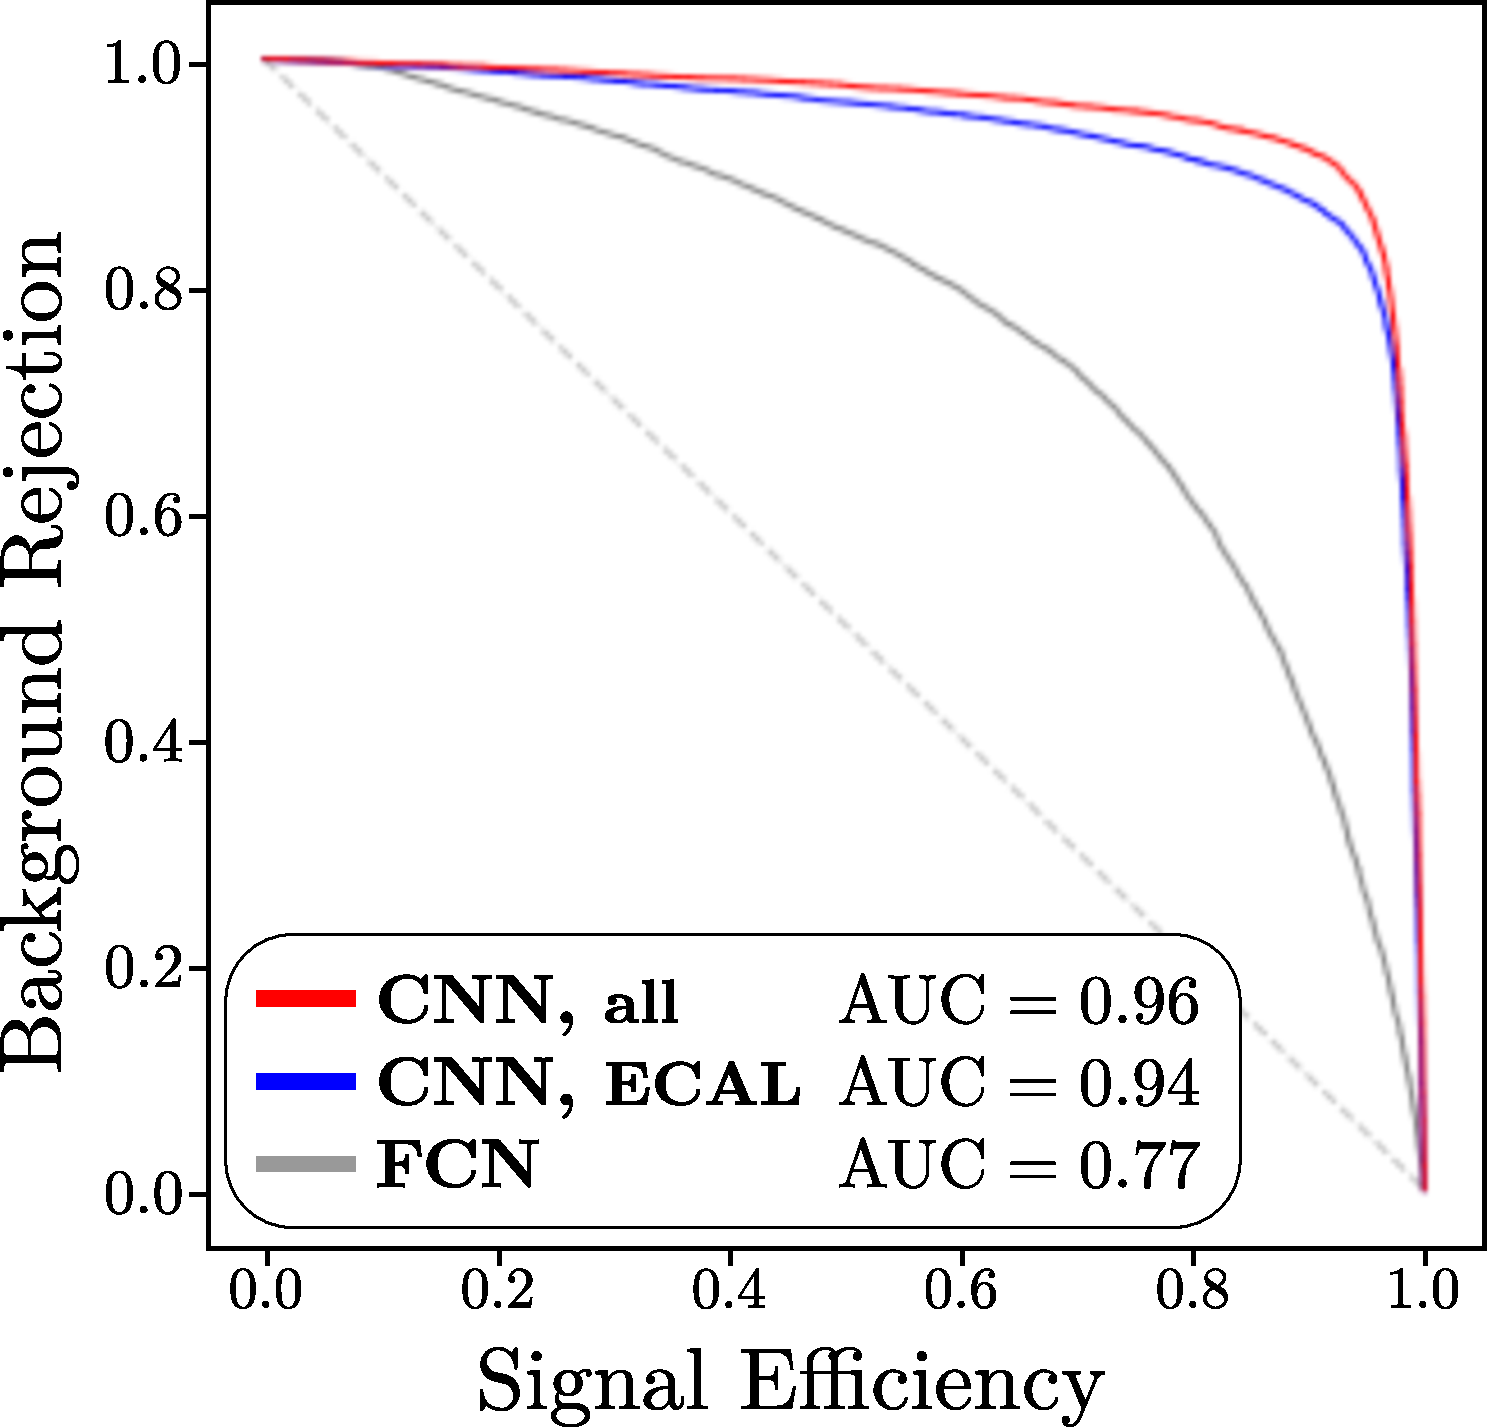
\includegraphics[width=\columnwidth]{raster/raster-svg/roc.pdf}
        \end{figure}

    \end{columns}

    \vfill
    {\tiny ROC curve adapted from \cite{andrews-higgs}}

\end{frame}

\begin{frame}
    \frametitle{Interpretation}
    

    \only<1>{
    Recall the input image...
    \begin{figure}[htb!]
        \centering
        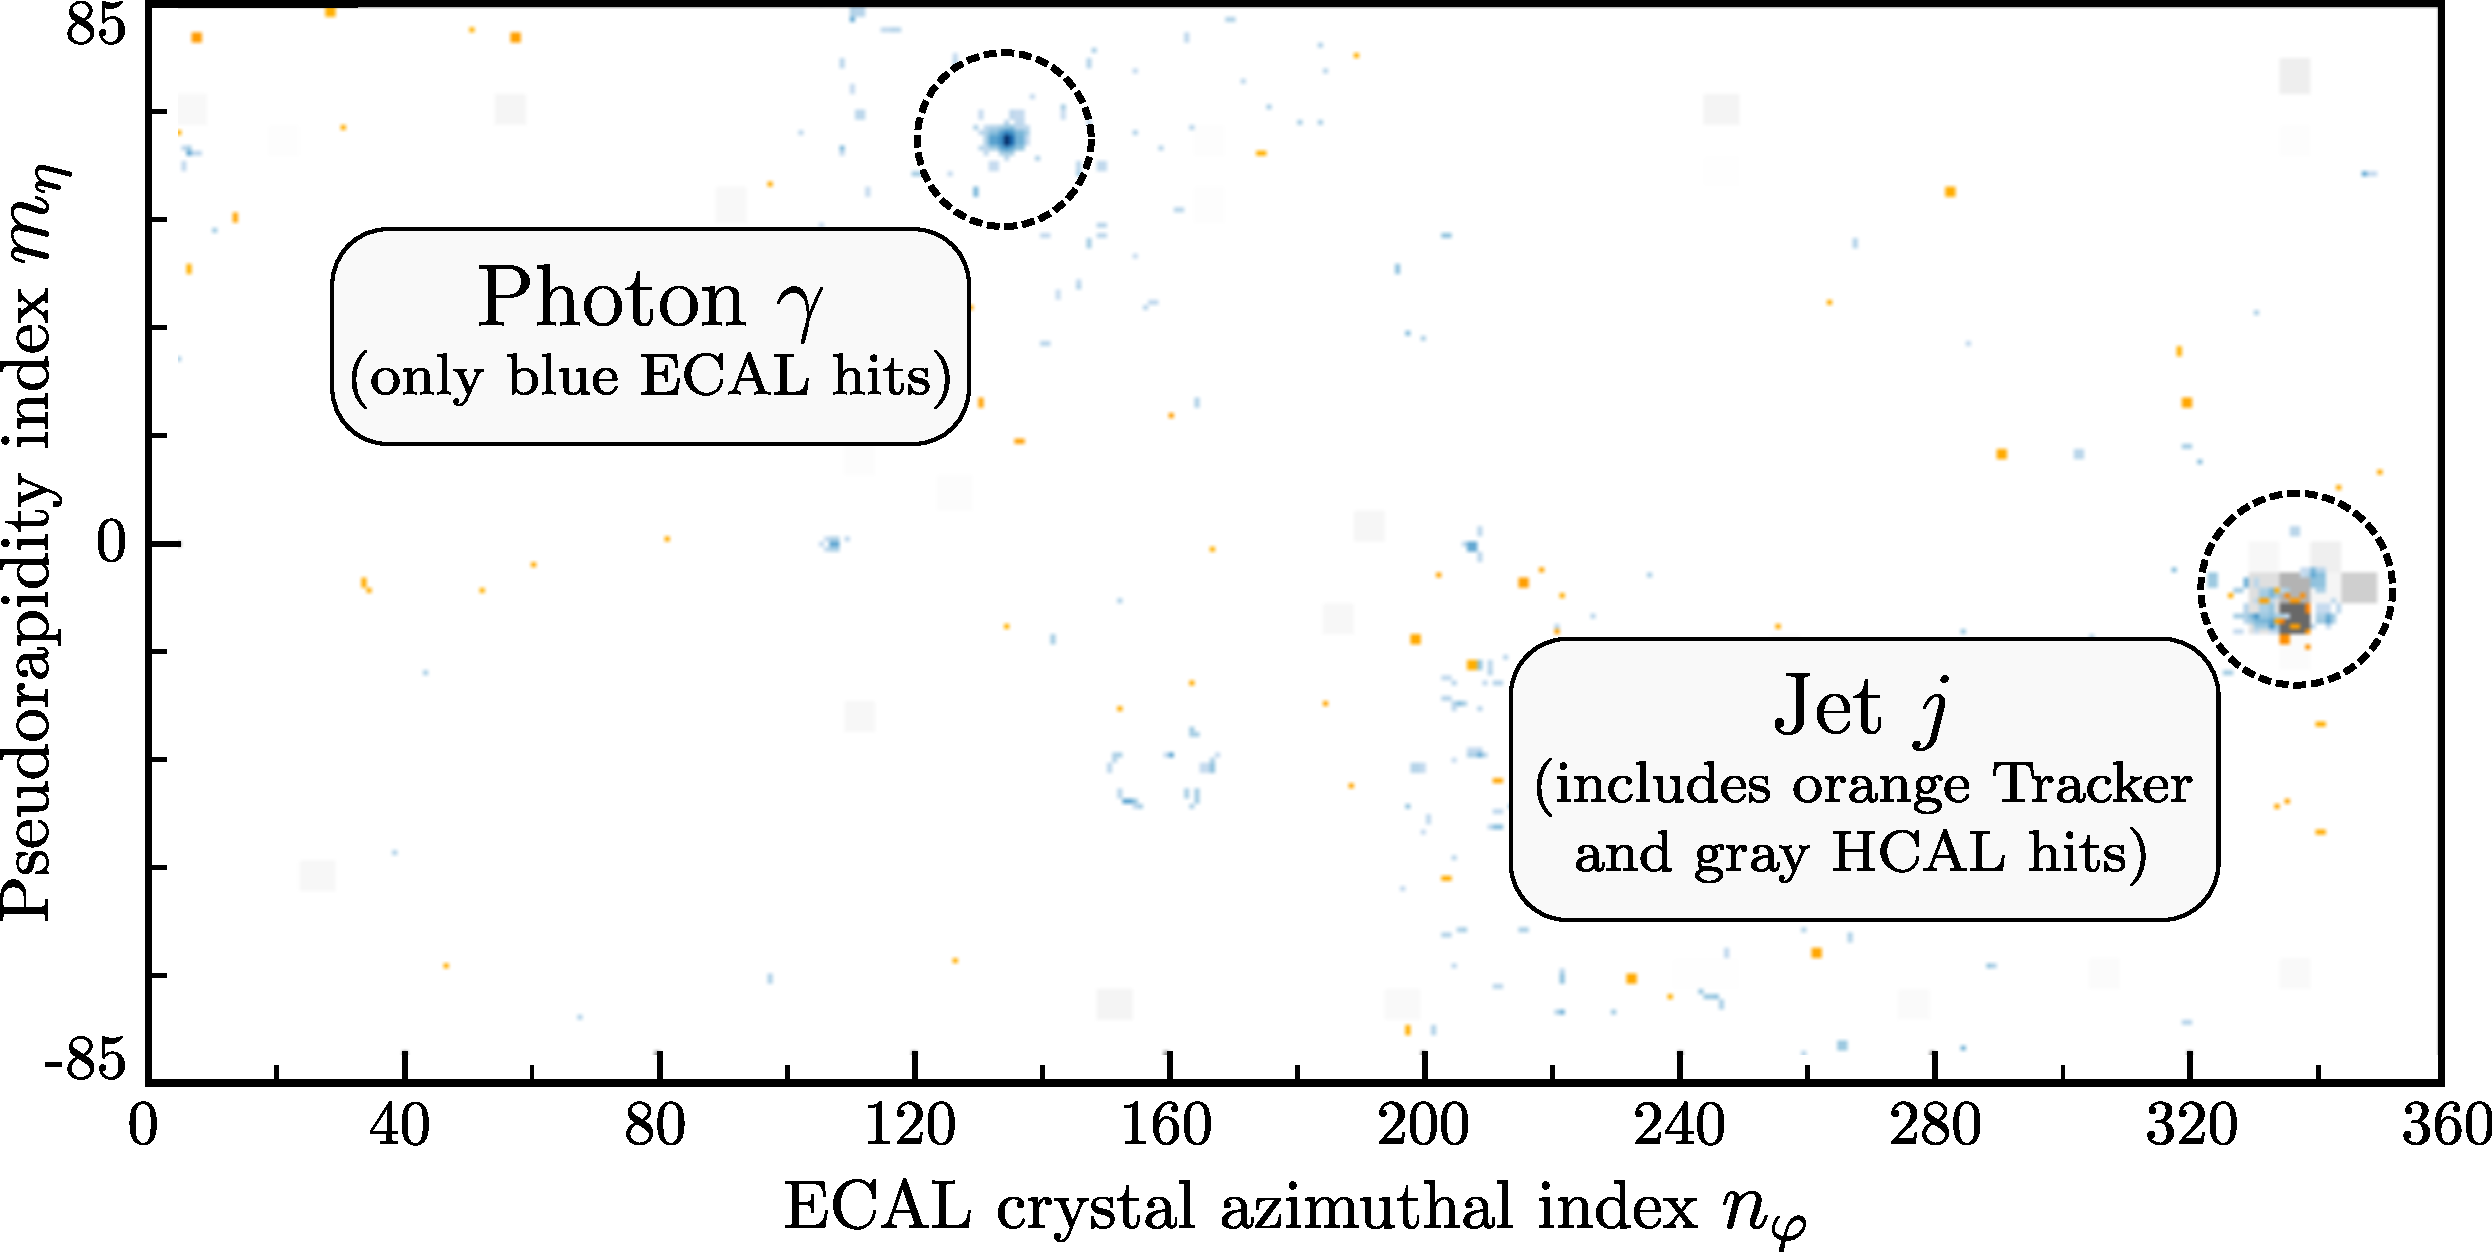
\includegraphics[width=\linewidth]{raster/raster-svg/event-image.pdf}
    \end{figure}}

    \only<2>{
    \begin{columns}

        \column{0.5\linewidth}
        {\centering \textbf{What a CNN sees}}

        \begin{figure}[htb!]
            \centering
            
\includegraphics[width=\columnwidth]{raster/raster-svg/photon-jet.pdf}
        \end{figure}

        \column{0.5\linewidth}
        {\centering \textbf{What a FCN sees}}
        \vspace{3mm}
        \begin{alignat*}{2}
            && p_{\text{T}} & \approx \SI{55}{\giga \electronvolt}\\
            && \varphi & \approx \ang{136} \\
            && \eta & \approx 1.10 \quad (\theta \approx \ang{37}) \\[16mm]
            && p_{\text{T}} & \approx \SI{65}{\giga \electronvolt}\\
            && \varphi & \approx \ang{335} \\
            && \eta & \approx -0.14 \quad (\theta \approx \ang{98})
        \end{alignat*} 
    \end{columns}}

    \only<3>{
    \begin{columns}

        \column{0.5\linewidth}
        {\centering \textbf{What a CNN sees}}

        \begin{figure}[htb!]
            \centering
            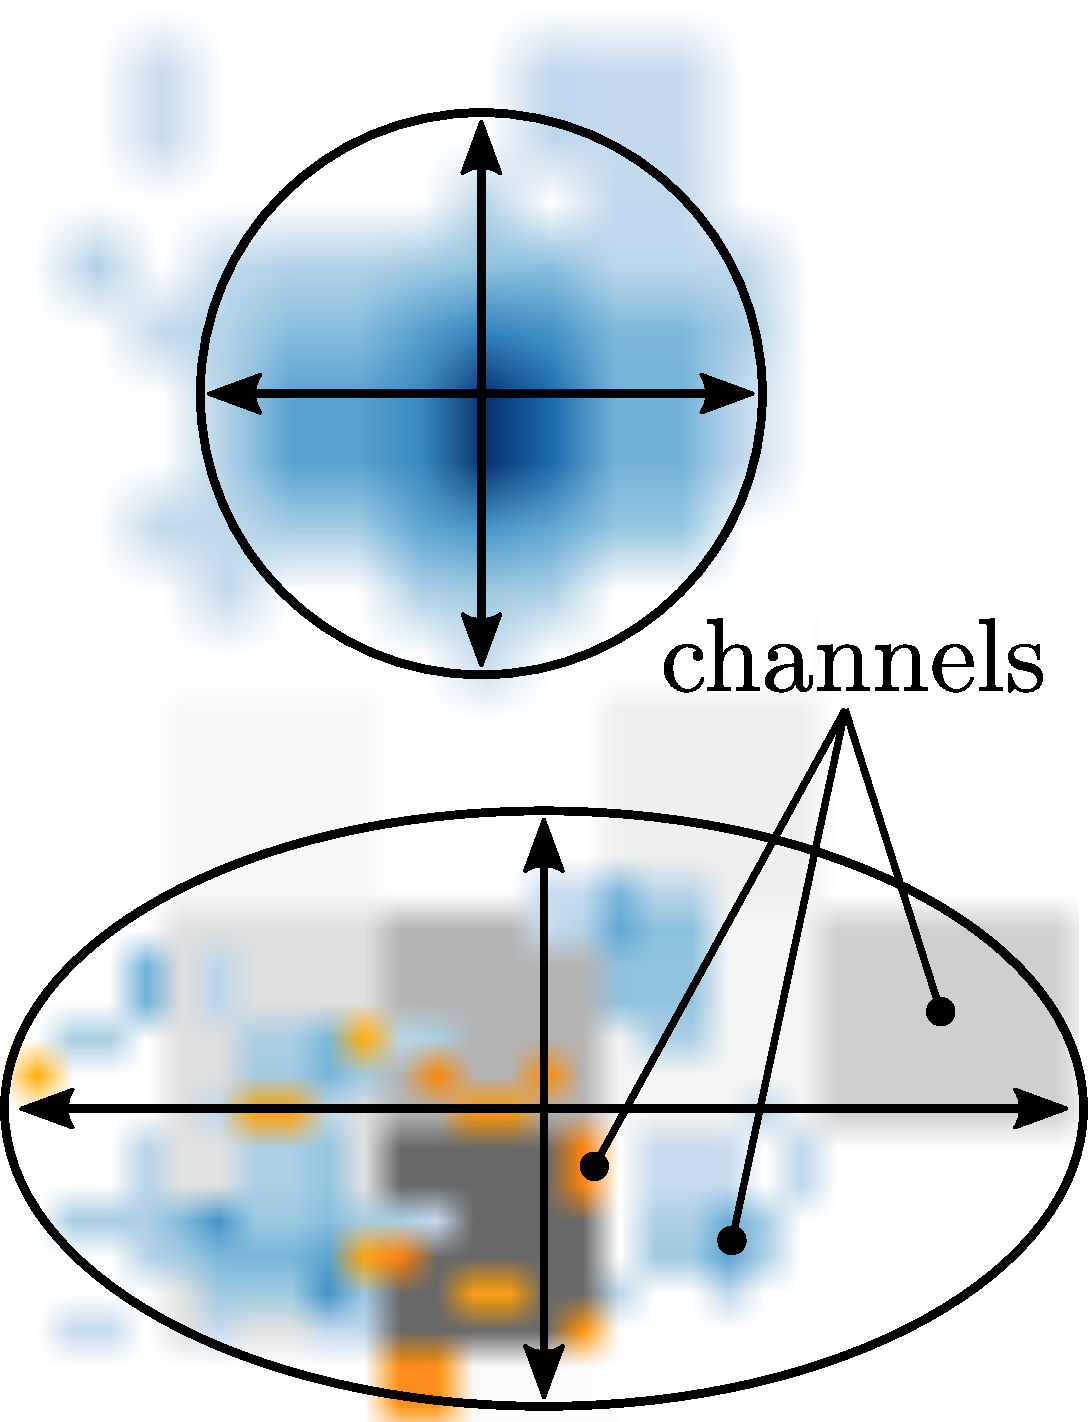
\includegraphics[width=\columnwidth]{raster/raster-svg/photon-jet-annotated.pdf}
        \end{figure}

        \column{0.5\linewidth}
        {\centering \textbf{What a FCN sees}}
        \vspace{3mm}
        \begin{alignat*}{2}
            && p_{\text{T}} & \approx \SI{55}{\giga \electronvolt}\\
            && \varphi & \approx \ang{136} \\
            && \eta & \approx 1.10 \quad (\theta \approx \ang{37}) \\[16mm]
            && p_{\text{T}} & \approx \SI{65}{\giga \electronvolt}\\
            && \varphi & \approx \ang{335} \\
            && \eta & \approx -0.14 \quad (\theta \approx \ang{98})
        \end{alignat*} 
    \end{columns}}

\end{frame}

\begin{frame}
    \frametitle{Takeaways and Conclusion}

    \begin{center}
        CNNs can distinguish shower distribution patterns even when kinematic quantities are identical.
    \end{center}
    \underline{Promising aspects of end-to-end classification}
    \vspace{1mm}
    \begin{itemize}
    
        \item Preserve maximum available information
        \vspace{0.5mm}

        \item Learn from spatial distribution
        \vspace{0.5mm}

        \item Flexible and general classification framework 
    
    \end{itemize}

    \pause
    \vspace{2mm}
    \begin{center}
        \Large{Thank you!}
    \end{center}
    
\end{frame}

\begin{frame}
    \frametitle{References}
    \printbibliography
\end{frame}

\end{document}
